\documentclass[color]{tudbook}
\usepackage{tudthesis}

\usepackage[ngerman,english]{babel}
\usepackage[T1]{fontenc}
\usepackage[latin1]{inputenc}

\usepackage{listings}
\usepackage{graphicx}
\usepackage{eso-pic}
\usepackage{pstricks}
\usepackage{listings}
\usepackage{floatflt}
\usepackage{rotating}

% Used for a list of abbreveations. %
\usepackage[printonlyused]{acronym}
	
\definecolor{darkgreen}{rgb}{0,0.5,0}


% F�r listings
\usepackage{listings}
\lstset{
  frame=single,
  frameround=tttt,
  xleftmargin=0.7cm,
  xrightmargin=0.3cm,
  numbers=left,
  basicstyle=\fontfamily{pcr} \small \color{black},
  keywordstyle=\bfseries \color{blue},
	stringstyle=\color{red},
	commentstyle=\color{darkgreen},
	breaklines=true,
	showstringspaces=false
}

\newcommand{\model}[1]{{\begin{ttfamily}#1\end{ttfamily}}}
\newcommand{\code}[1]{{\begin{ttfamily}#1\end{ttfamily}}}
\newcommand{\reference}[1]{{\begin{ttfamily}#1\end{ttfamily}}}
\newcommand{\keyword}[1]{{\begin{itshape}#1\end{itshape}}}
\newcommand{\eclipse}[1]{{\begin{itshape}#1\end{itshape}}}

% Define Faculty and Institute
\einrichtung{Faculty of Computer Science}
\institut{Institute of Software- and Multimedia-Technology}
\professur{Software Technology Group}

% Define the title of the manual
\title{Dresden OCL}
\subtitle{Manual for Installation, Use and Development}
% Specify the author of the manual
\author{Claas Wilke, Michael Thiele, Bj\"{o}rn Freitag, and Lars Sch\"{u}tze}
% Specify the date at that the manual changed the last time
\date{Last update: \today}

% F�r Metadaten im PDF.
\usepackage[
  bookmarksnumbered=true,
  pdftitle={Dresden OCL - Manual},
  pdfauthor={Claas Wilke},
  pdfcreator={TeXnicCenter},
  pdfkeywords={OCL, Dresden OCL, constraints},
  pdfsubject={The Dresden OCL Manual}
]{hyperref}

\hypersetup{
  colorlinks=true,
  linkcolor=HKS41-100,
  citecolor=HKS41-100,
  filecolor=HKS41-100,
  menucolor=HKS41-100,
  urlcolor=HKS41-100
} 


\newcommand{\todo}[1]{\color{red}\textbf{TODO #1}\color{black}}
\newcommand{\todocw}[1]{\todo{Claas: #1}}
\newcommand{\todomt}[1]{\todo{Micha: #1}}

\begin{document}


\maketitle

Dresden OCL has been developed at the Technische Universit�t Dresden,
Department of Computer Science, Software Technology Group. Dresden OCL and this
manual are available a the Dresden OCL project website
(\url{http://www.dresden-ocl.org/}).



\section*{Contact}

Technische Universit�t Dresden \newline
Fakult�t Informatik\newline
Lehrstuhl Softwaretechnik\newline
Prof. Dr. Uwe A�mann\newline
N�thnitzer Str. 46\newline
D-01187 Dresden



\section*{License}

We are always looking forward to find new projects that use Dresden OCL or at
least parts of it. Thus, please inform us, if you use Dresden OCL wthin your
project, tool or application.


\subsection*{Dresden OCL}

\begin{floatingfigure}[r]{2.0cm}
	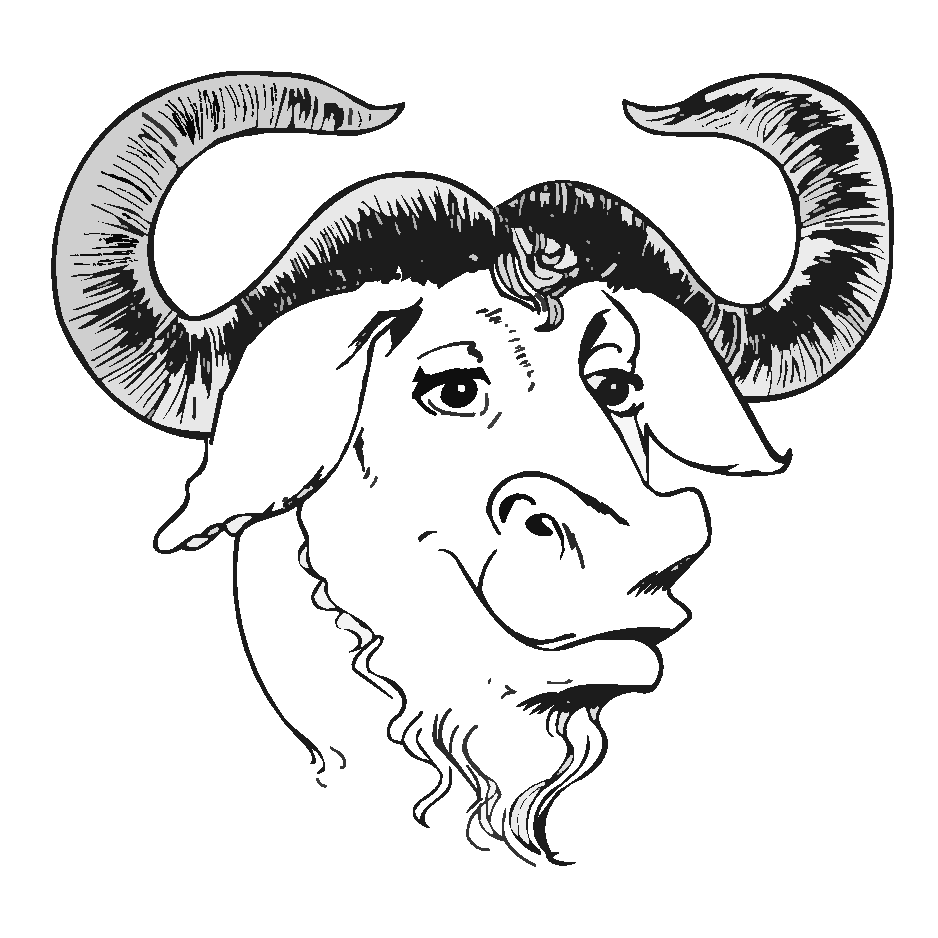
\includegraphics[width=2.0cm]{figures/license/gnu.pdf}
\end{floatingfigure}

Dresden OCL is free software: you can redistribute it and/or modify it under the terms of the \keyword{GNU Lesser General Public License} as published by the \keyword{Free Software Foundation}, either version 3 of the License, or (at your option) any later version. Dresden OCL is distributed in the hope that it will be useful, but \textbf{without any warranty}; without even the implied warranty of \textbf{merchantability} or \textbf{fitness for a particular purpose}. See the GNU Lesser General Public License for more details. You should have received a copy of the GNU Lesser General Public License along with Dresden OCL. If not, see \url{http://www.gnu.org/licenses/}.


\subsection*{This Manual}

\begin{floatingfigure}[r]{1.5cm}
	
\includegraphics[width=1.5cm]{figures/license/by.pdf}
\end{floatingfigure}

This document is licensed under the \keyword{Creative Commons Attribution 3.0 Unported} license. 
You may share, copy, distribute and transmit this document and you can also adapt this document into your own work. But be aware that you must attribute the work in the manner specified by the author or licensor (but not in any way that suggests that they endorse you or your use of the work). The full license is available under \url{http://creativecommons.org/licenses/by/3.0/}.

\begin{abstract}
\addcontentsline{toc}{chapter}{Abstract}
This document contains the documentation of DresdenOCL. In the first part of
this manual the general use of DresdenOCL is explained. Afterwards, use cases
like \acs{OCL} interpretation and code generation are presented. The second part
of this manual contains the technical documentation of DresdenOCL, like its
architecture and the adaptation of further types of models and model instances
to DresdenOCL.

Please be aware that DresdenOCL is a project developed at the Technische
Universit�t Dresden, Software Technology Group. Parts of the project have been 
designed and implemented during student theses and have been developed as
prototypes only. Thus, DresdenOCL is far from being complete. To report bugs 
and errors or request additional features or answers to specific questions visit
DresdenOCL's website~\cite{WWW:toolkit} or the project site at
\keyword{Sourceforge}~\cite{WWW:toolkitSourceforge}.

The procedure's described in this manual were run and tested with
\keyword{Eclipse 3.6}~\cite{WWW:eclipse}. We recommend to use the 
\keyword{Eclipse Modeling Tools Edition} which contains most required plug-ins
to run DresdenOCL. Otherwise you need to install at least the plug-ins enlisted
in Table \ref{tab:software}. Alternatively, DresdenOCL may be used as a
stand-alone library for Java. If you want to use the stand-alone distribution, 
you cannot use the \acs{GUI}s and editors provided with DresdenOCL since the GUI
elements depend on Eclipse. The use of the stand-alone distribution is
documented in Chapter~\ref{chapter:standalone}.

\end{abstract}


\tableofcontents


\part{Using Dresden OCL}

\chapter{About Dresden OCL}
\label{chapter:about}

\begin{flushright}
\textit{Chapter written by Claas Wilke and Michael Thiele}
\end{flushright}

\emph{DresdenOCL} is developed as a project at the Technische Universit�t 
Dresden (TUD), Software Technology Group since 1999. Its latest version is 
released as a set of Eclipse plug-ins and thus, called \emph{\acl{DOT4Eclipse}}.
DresdenOCL contains a set of OCL tools, including an OCL parser, an OCL
interpreter and an OCL-to-Java code generator.
\todocw{Mention the OCL22SQL code generator here when available.}

In this chapter, some general information on DresdenOCL is presented. The 
supported OCL version and the differences to the official OCL specification are 
documented. Supported meta-models, models and model instances are shortly
presented. If you are not interested in such information, you can skip this 
chapter and continue with the installation and general use of DresdenOCL as 
documented in Chapter~\ref{chapter:introduction}.
  


\section{Supported Version of OCL}

DresdenOCL generally supports OCL 2.2 as specified in \cite{spec:OCL2-2}. 
Nevertheless, some differences between DresdenOCL and OCL 2.2 exist as
documented in the following:


\subsection{Comformance of DresdenOCL to the OCL 2.2 specification}

The OCL 2.2 specification defines a set of compliance points that can be
addressed by tools implementing OCL~\cite[p.~1]{spec:OCL2-2}.
Table~\ref{tab:compliance} summarises the compliance points addressed by
DresdenOCL.

\begin{table}[h]
\begin{tabular}{|p{7cm}|p{7cm}|}
    \hline
    \textbf{Compliance Point} & \textbf{Support in DresdenOCL} \\
    \hline
    Syntax & 
    Fully supported (Except OclMessage and related operations) \\
    \hline
    XMI & 
    XMI export import of OCL is currently not supported \\
    \hline
    Evaluation & 
    \\
    - allInstances() &
    supported \footnotesize(with some limitations to specific
    technological spaces, e.g., Java) \\
    - @pre in postconditions &
    supported \\
    - OclMessage & 
    not supported \\
    - Navigating non-navigable association ends & 
    not supported \\
    - accessing private and protected features & 
    supported \\
    \hline
\end{tabular}
\caption{Compliance points addressed by DresdenOCL (v. 3.0.0) according
to~\cite[p.~1]{spec:OCL2-2}.}
\label{tab:compliance}
\end{table}
	
	
\subsection{Different Semantics of OCL Expressions in DresdenOCL}

The current OCL 2.2 specification~\cite{spec:OCL2-2} contains some
inconsistencies and misses some definitions especially when evaluating
\code{invalid} or \code{null} values. Thus, we had to assume or change the
semantics of OCL during evaluation of some OCL statements. In the following
we present the differences of the OCL semantics used in DresdenOCL compared 
with the official OCL specification~\cite{spec:OCL2-2}.


\subsubsection{Boolean Operators}

\begin{table}
	\centering
		\begin{tabular}{|p{1.2cm}p{1.2cm}||p{1.2cm}|p{1.2cm}|p{1.2cm}|p{1.2cm}|p{2.0cm}|}
			\hline
      \textbf{a}	& \textbf{b}	& \textbf{not a}	& \textbf{a or b}	& \textbf{a xor b} 	& \textbf{a and b}	& \textbf{a implies b} \\
			\hline
			false				&	false				&	true						&	false						& false							&	false							&	true \\
			\hline	
			false				&	true				&	- `` -						&	true						& true							&	false							&
			true
			\\
			\hline
			false				&	null				&	- `` -							&	invalid					& invalid						&	false							&	true \\
			\hline
			false				&	invalid			&	- `` -							&	invalid					& invalid						&	false							&	true \\
			\hline
			true				&	false				&	false						&	true						& true							&	false							&	false \\
			\hline
			true				&	true				&	- `` -							&	true						& false							&	true							&	true \\
			\hline
			true				&	null				&	- `` -							&	true						& invalid						&	invalid						&	invalid \\
			\hline
			true				&	invalid			&	- `` -							&	true						& invalid						&	invalid						&	invalid \\
			\hline
			null				&	false				&	invalid					&	invalid					& invalid						&	false							&	invalid \\
			\hline
			null				&	true				&	- `` -							&	true						& invalid						&	invalid						&	invalid \\
			\hline
			null				&	null				&	- `` -							&	invalid					& invalid						&	invalid						&	invalid \\
			\hline
			null				& invalid			&	- `` -							&	invalid					& invalid						&	invalid						&	invalid \\
			\hline
			invalid			& false				&	invalid					&	invalid					& invalid						&	false							&	invalid \\
			\hline
			invalid			&	true				&	- `` -							&	true						& invalid						&	invalid						&	invalid \\
			\hline
			invalid			&	null				&	- `` -							&	invalid					& invalid						&	invalid						&	invalid \\
			\hline
			invalid			&	invalid			&	- `` -							&	invalid					& invalid						& invalid						&	invalid \\
			\hline
		\end{tabular}
		\caption{Decision Table for boolean operators in Dresden OCL.}
		\label{tab:decisionTable}
\end{table}

Boolean operators in DresdenOCL are interpreted as documented in 
Table~\ref{tab:decisionTable}. As documented, the operator \code{and} always 
results in \code{false} as long as one of its operands is \code{false}, ignoring
whether the other operand is \code{null} or even \code{invalid}. The operator 
\code{or} results in \code{true}, as long as one of its operands is \code{true}.
Both \code{false implies null} and \code{false implies invalid} result in 
\code{true}. The operator \code{xor} can only be evaluated if both arguments 
are neither \code{null} nor \code{invalid}. Otherwise the operand will result in
\code{invalid}.


\subsubsection{Equality in DresdenOCL}

\begin{table}
	\centering
		\begin{tabular}{|p{1.2cm}p{1.2cm}||p{1.2cm}|p{1.2cm}|p{1.2cm}|p{1.2cm}|p{1.2cm}|p{1.2cm}|}
			\hline
      \textbf{a} 	& \textbf{b} 	& \textbf{a = b} 	& \textbf{a <> b} 	& \textbf{a < b} 	& \textbf{a <= b} 	& \textbf{a > b} 	& \textbf{a >= b} \\
			\hline
			42					&	42					&	true						&	false							&	false						&	true							&	false							&	true \\
			\hline
			42					&	7						&	false						&	true							&	false						&	false							&	true							&	true \\
			\hline
			42					&	null				&	false						&	true							&	invalid					&	invalid						&	invalid						&	invalid \\
			\hline
			null				&	null				&	true						&	false							&	invalid					&	invalid						&	invalid						&	invalid \\
			\hline
			42					&	invalid			&	false						&	true							&	invalid					&	invalid						&	invalid						&	invalid \\
			\hline
			invalid			&	invalid			&	true						&	false							&	invalid					&	invalid						&	invalid						&	invalid \\
			\hline
		\end{tabular}
		\caption{Decision Table for equality operators in Dresden OCL.}
		\label{tab:info:equalityDecisionTable}
\end{table}

\acs{OCL} defines the two operators \code{=} and \code{<>} to compute equality 
of two given \acs{OCL} expressions. Since \acs{OCL} values can be both
\code{null} or \code{invalid}, it is important to know how these operators 
behave when used with \code{null} and \code{invalid} values. According to the 
specification, comparing two \acs{OCL} values results in an illegal state when 
one of the two values is either \code{null} or \code{invalid}. However, it is
not specified if the comparison results in \code{null} or 
\code{invalid}~\cite[p. 195]{spec:OCL2-2}. In some situations this can lead to 
problems during evaluation, e.g., when iterating on an \acs{OCL} collection 
containing \code{null} values.

Thus in DresdenOCL, using the operators \code{=} and \code{<>} for comparison
will always result in \code{true} or \code{false} as documented in 
Table~\ref{tab:info:equalityDecisionTable}. But please be aware, that this 
behaviour is only implemented for \code{=} and \code{<>}. Using other comparison
operators such as \code{<}, \code{<=}, \code{>}, and \code{>=} for numeric 
values can result in \code{invalid}!


\subsubsection{Collections}

In DresdenOCL, collections can contain \code{null} values but cannot contain 
\code{invalid} values! If an \code{invalid} value is contained in a collection, 
the complete collection will be \code{invalid} as well.


\subsubsection{Iterators}

\begin{figure}[t]
\lstset{keywords={Bag, true, false, invalid, null}, label={lst:exampleIterators}, caption={Some example Iterator Expressions and their evaluation results.}, captionpos=b}
\begin{lstlisting}
Bag { true, null } -> exists(true) => true
Bag { true, null } -> forAll(true) => invalid
Bag { true, null } -> one(true) => true
Bag { true, null } -> one(false) => invalid
Bag { true, null } -> select(true) => invalid
Bag { true, null } -> select(oclIsUndefined()) => Bag { null }
\end{lstlisting}
\end{figure}

In DresdenOCL, iterators will result in a value as long as they can be computed,
even if their collection contains \code{null} values. 
Listing~\ref{lst:exampleIterators} shows some examples for iterator expressions 
and their results in DresdenOCL. E.g., an \code{any} iterator will result in 
\code{true} as long as one element of its source's collection fulfils its 
condition even if other elements are \code{null} values. On the other hand, a 
\code{select} iterator will result in \code{invalid} if the condition for any 
element in its collection results in \code{null}. However, if the collection 
contains \code{null} values but the condition results in \code{true} or 
\code{false} (e.g., \code{oclIsUndefined()}), the result will not be 
\code{invalid}.


\subsubsection{Handling of Null values}

\begin{figure}[t]
\lstset{keywords={Bag, true, false, invalid, null}, label={lst:info:nullValues}, caption={Evaluation of null values in DresdenOCL.}, captionpos=b}
\begin{lstlisting}
null + 2 => invalid
null.asSet() => Set { }
null.oclIsUndefined() => true
invalid.oclIsUndefined() => invalid
\end{lstlisting}
\end{figure}

According to the OCL 2.2 specification~\cite{spec:OCL2-2}, all operation calls
invoked on \code{null} values will result in \code{invalid}. An exception is the
operation \code{oclIsUndefined()} which results in \code{true} if its source is 
\code{null} and \code{false} otherwise. According to the OCL 2.2 specification 
the expression \code{invalid.oclIsUndefined()} will result in \code{true} as
well. \textbf{In DresdenOCL, \code{invalid.ocl\-Is\-Undefined()} results in 
\code{invalid} instead!} According to the OCL 2.2. specification, the implicit 
OCL operation \code{asSet()} can be invoked on \code{null} values and will
result in an empty \code{Set}. Listing~\ref{lst:info:nullValues} shows some
examples for evaluations on \code{null} values.


\subsubsection{Handling of Invalid values}

\begin{figure}[t]
\lstset{keywords={Bag, true, false, invalid, null}, label={lst:info:invalidValues}, caption={Evaluation of invalid values in DresdenOCL.}, captionpos=b}
\begin{lstlisting}
invalid + 2 => invalid
invalid.asSet() => invalid
invalid.oclIsInvalid() => true
undefined.oclIsInvalid() => false
\end{lstlisting}
\end{figure}

According to the OCL 2.2 specification~\cite{spec:OCL2-2}, all operation calls 
invoked on \code{invalid} values will result in \code{invalid}. Exceptions are 
the operations \code{oclIsInvalid()} and \code{oclIsUndefined()}. The evaluation
of \code{oclIsInvalid()} will result in \code{true} when invoked on 
\code{invalid} values. Otherwise it will result in \code{false}, even when 
invoked on \code{null} values. \code{invalid.asSet()} will result in 
\code{invalid} because sets cannot contain invalid values. 
Listing~\ref{lst:info:invalidValues} shows some examples for evaluations on 
\code{invalid} values.



\section{Supported Models In Dresden OCL}
\label{sect:info:models}

DresdenOCL is adapted to multiple meta-models and thus allows the import of 
multiple kinds of models. Which kinds of models and which model file formats are
supported by DresdenOCL is documented in this section.


\subsection{EMF Ecore Models}

DresdenOCL allows to import Ecore models modelled with the
\emph{\acf{EMF}}~\cite{WWW:EMF}. Typically, Ecore models are stored in \acs{XMI}
files matching to the naming pattern \code{*.ecore}.


\subsection{Java Classes as Models}

DresdenOCL supports to import Java classes as models and thus to define
\acs{OCL} constraints directly on Java types and their fields and methods. If a 
Java class is imported into DresdenOCL, all types used inside the class' 
declaration are handled as also being a part of the imported model. If a 
\code{ClassA} is imported into DresdenOCL containing an attribute of the type 
\code{ClassB}, \code{ClassB} is also imported into DresdenOCL. \code{ClassB} 
could contain an operation having the return type \code{ClassC} and thus 
\code{ClassC} could be imported as well. After short consideration it should be 
clear that such a transitive mechanism could lead to a more or less complete
import of the Java standard library into DresdenOCL. Thus, only the types that 
are used during OCL parsing and evaluation are imported into DresdenOCL.

\begin{figure}[t]
\lstset{language=Java, label={lst:javaModelProvider}, caption={Example for a Java Model Provider Class.}, captionpos=b}
\begin{lstlisting}
package tudresden.ocl20.pivot.examples.simple;

public class ModelProviderClass {

  protected Person person;

  protected Professor professor;

  protected Student student;
}
\end{lstlisting}
\end{figure}

If a \code{ClassA} is imported into DresdenOCL, the type of \code{ClassA} and
all types that are directly related to this class are imported as well. E.g., a 
\code{ClassB} used in a property of \code{ClassA} would be imported, a related 
\code{ClassC} used in \code{ClassB} would not be imported (see 
Figure~\ref{fig:info:transitiveTypeImport}). If other types are requested during
the work of tools on the imported model (e.g., if a tool requests the operation 
\code{ClassB.getOwnedOperations()}, all newly required types will be imported as
well. This deferred transitive adaptation mechanism avoids that all types never 
used inside DresdenOCL are imported and adapted and cause overhead and
maintenance problems. Listing~\ref{lst:javaModelProvider} shows an example for a
Java class provided with the \emph{Simple Example} of DresdenOCL. The class
contains properties having the types \code{Person}, \code{Professor} and 
\code{Student}. Thus, the imported model in DresdenOCL will contain a package 
\code{tudresden.ocl20.pivot.example.simple}, containing the four classes 
\code{ModelProviderClass} \code{Person}, \code{Professor} and \code{Student}.

\begin{figure}[t]
	\centering
		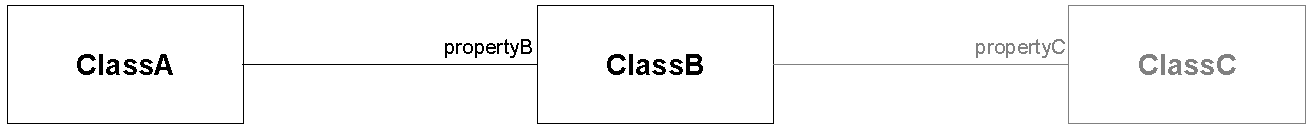
\includegraphics[width=1.00\textwidth]{figures/info/transitiveTypeImport.pdf}
	\caption{Transitive Import of Java Classes as a Model into DresdenOCL.}
	\label{fig:info:transitiveTypeImport}
\end{figure}

To import Java classes into DresdenOCL two possibilities exist:

\begin{enumerate}
	\item \code{*.class} files can be imported as a model. All directly referenced 
	  classes (either as types of properties and operations or their arguments) are
	  imported as well. \textbf{Please be aware, that only byte code classes
	  (\code{*.class}) and not source code classes \code{*.java} can be imported
	  into DresdenOCL!}
	\item Alternatively, the path leading to the Java class to be imported can be 
	  declared in a text file matching to the file naming pattern
	  \code{*.javamodel}. This alternative was implemented to support the import of
	  Java classes referencing other external Java classes provided as \acs{JAR}s.
	  An example for a \code{*.javamodel} text file is shown in 
	  Listing~\ref{lst:javaModel}. The first line references the 
	  \code{JarClassProvider.class} that shall be imported as a model. The second 
	  line references a \acs{JAR} file that contains classes whose types are 
	  referenced in the \code{JarClassProvider.class}. Both, the class and the 
	  \acs{JAR} are referenced via relative \acs{URL}s from the directory where the
	  \code{*.javamodel} file is located in the file system. Further lines of the 
	  \code{*.javamodel} text file could be used to reference additional \acs{JAR}s
	  to be imported as well. Please be aware, that only referenced classes from 
	  the \acs{JAR}s are imported into DresdenOCL. Again, further classes are 
	  imported when required during \acs{OCL} parsing or evaluation.
\end{enumerate}

\begin{figure}[t]
\lstset{language=OCL, label={lst:javaModel}, caption={Example for a .javamodel File.}, captionpos=b}
\begin{lstlisting}
../bin/package1/package2/JarClassProvider.class
../lib/simple.jar
\end{lstlisting}
\end{figure}


\subsection{MDT UML Class Diagrams}

DresdenOCL allows to import UML class diagrams modelled with the 
\emph{\acf{Eclipse MDT}}~\cite{WWW:MDT}. Typically, \acs{MDT} \acs{UML} models
are stored as \acs{XMI} files matching to the naming pattern \code{*.uml}. 
Since many Eclipse-based modelling tools built on top of \acs{MDT} \acs{UML}, 
their models can be imported as well. Examples for such modelling tools are the 
\emph{\acf{GMF}} \acs{UML} class diagram editor and the \emph{Topcased}
\acs{UML} class diagram editor.


\subsection{XML Schemas as Models}

DresdenOCL allows to import \acl{XSD}s (\acs{XSD}) as models. Typically, 
\acs{XSD}s are stored in \acs{XML} files matching to the naming pattern 
\code{*.xsd}.



\section{Supported Model Instances In Dresden OCL}
\label{sect:info:modelinstances}

DresdenOCL is adapted to and thus allows the import of multiple types of model 
instances. Which types of model instances are supported by DresdenOCL is 
documented in this section.


\subsection{EMF Ecore-Based Model Instances}

Besides the creation of meta-models or \acs{DSL}s, the \acf{EMF} allows the 
generation of simple model editors that can be used to model instances of the 
Ecore-based models created before. E.g., you can create a simple \acs{DSL} 
using \acs{EMF}. Afterwards you can model an instance of this \acs{DSL} using 
an Ecore-generated model editor. Now, you can import your \acs{DSL} as a model 
into DresdenOCL and you can parse \acs{OCL} constraints defined on your
\acs{DSL}. To check these constraints on the created model instance, you have to
import this instance into DresdenOCL as well.

Thus, DresdenOCL allows to import instances of Ecore-based models as model
instances. Typically, the instances are stored as \acs{XMI} files that match to
a file naming pattern that ends with the name of your Ecore model. E.g., if you 
modelled an \code{myDSL.ecore} and created an instance of this model via an 
Ecore-generated model editor, the instance matches to the naming pattern 
\code{*.mydsl}.

Besides complete models it can be useful to import single model instance
elements into Dres\-den\-OCL when using DresdenOCL directly from another
software application via its \acs{API}. How this is possible is documented in 
Section~\ref{sect:modelInstanceTypeAdaptation:addIMIElement}. For Ecore model 
instances, this mechanism can be used to add single \code{EObjects} to a model 
instance in DresdenOCL.


\subsection{Java Model Instances}

Java objects can be regarded as instances of model elements described in class 
diagrams or similar models. Thus, the import of Java objects as model instances 
for \acs{OCL} constraint interpretation is a common use case. DresdenOCL 
supports two possibilities to import Java objects into DresdenOCL.

\begin{figure}[t]
\lstset{language=Java, label={lst:info:javaModelInstance}, caption={Example for a ModelInstanceProviderClass programmed in Java.}, captionpos=b}
\begin{lstlisting}
public class ModelInstanceProviderClass {

  /**
   * @return A {@link List} of {@link Object}s that are part of the
   *         {@link IModelInstance}.
   */
  public static List<Object> getModelObjects() {

    List<Object> result;
    result = new ArrayList<Object>();

    Person person1;
    person1 = new Person();
    person1.setName("Person Unspecific");
    person1.setAge(25);
    result.add(person1);

    /* Add further elements ... */
		
    return result;
  }
}
\end{lstlisting}
\end{figure}

\begin{enumerate}
	\item It is possible to create a \code{ModelInstanceProviderClass} containing
	  a static method called \code{getModelObjects()} that returns a \code{List} of
	  \code{java.lang.Objects} that shall be imported as a model instance.
	  Listing~\ref{lst:info:javaModelInstance} shows an example of such a
	  \code{ModelInstanceProviderClass}.
	\item Similar to Ecore model instances, it is possible to add single 
	  \code{java.lang.Object}s to an existing model instance via DresdenOCL's
	  \acs{API} at runtime as documented in
	  Section~\ref{sect:modelInstanceTypeAdaptation:addIMIElement}.
\end{enumerate}


\subsection{XML Model Instances}

DresdenOCL supports to import \acs{XML} files as model instances. Although
\acs{XML} files cannot contain executable code, their elements can be used as
data to be verified by structural \acs{OCL} integrity constraints. Typically 
\acs{XML} files conform to the file name matching pattern \code{*.xml}.



\section{Summary}

This chapter documented which version of OCL is supported by DresdenOCL. 
Furthermore, supported types of models, and model instances were presented. The
following chapter will explain how to install and use DresdenOCL.

\chapter{Getting started with Dresden OCL}
\label{chapter:introduction}

\begin{flushright}
\textit{Chapter written by Claas Wilke and Michael Thiele}
\end{flushright}

This chapter generally introduces into \keyword{Dresden OCL}. Dresden OCL is
based on a \keyword{Pivot Model} developed by Matthias 
Br�uer~\cite{GB:Braeuer} which is shortly explained in 
Chapter~\ref{chapter:architecture}. Further information about Dresden OCL is 
available at the project's website~\cite{WWW:toolkit}.

This chapter explains the installation of Dresden OCL and how to load a 
model, an instance of such a model, and \acs{OCL} constraints defined on such a 
model into Dresden OCL. Besides the Eclipse distribution, Dresden OCL can 
also be used as a stand-alone Java library. If you plan to use the stand-alone 
distribution you can skip this chapter and continue with 
Chapter~\ref{chapter:standalone}. However, this chapter explains the basic 
concepts of Dresden OCL. Although you cannot use the shown GUI wizards and 
browsers when using the stand-alone version, this chapter can be helpful to 
understand the terms used in and the mechanisms provided by Dresden OCL.
  


\section{How to Install Dresden OCL}
	
The following different possibilities exist to install Dresden OCL within
Eclipse.

\begin{enumerate}
	\item You may install Dresden OCL using the \emph{Eclipse Marketplace
	  Client}.
	\item You may install Dresden using the update site available
	  at~\cite{WWW:toolkitUpdatesite},
	\item You may checkout and run the source code distribution from the \acs{SVN}
	  available at~\cite{WWW:toolkitSVN}.
\end{enumerate}

This section will explain all three possibilities.
	

\subsection{Installing Dresden OCL using the Eclipse Marketplace Client}

Since Eclipse 3.6, the new Eclipse Marketplace Client allows easy installation
of Eclipse-based tools such as Dresden OCL.

To install Dresden OCL via the Eclipse Marketplace Client, select the menu
option \emph{Help -> Eclipse Marketplace\ldots}. Probably you have to select a
marketplace catalog afterwards. If so, select the \emph{Eclipse Marketplace}
catalog and proceed.

Type \texttt{Dresden OCL} into the search text field and press the return key.
Select Dresden OCL from the search results and click the \emph{Install} button
(cf. Fig.~\ref{pic:intro:marketplace01}). Afterwards, click through the
installation dialog and Dresden OCL will be installed. Finally you have to 
restart your Eclipse distribution to complete the installation.

\begin{figure}[!b]
	\centering
	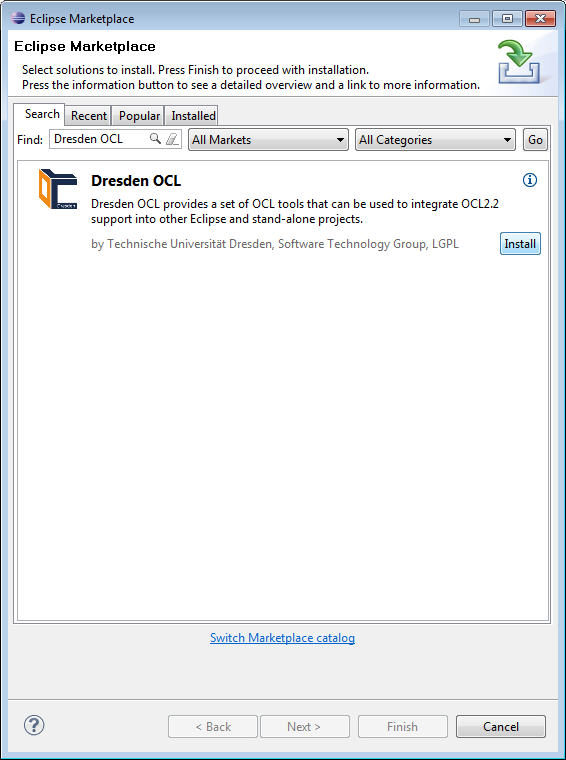
\includegraphics[width=0.8\linewidth]{figures/introduction/marketplace01}
	\caption{Installing Dresden OCL using the Marketplace Client.}
	\label{pic:intro:marketplace01}
\end{figure}


\subsection{Installing Dresden OCL using the Eclipse Update Site}
	
To install Dresden OCL via the \keyword{Eclipse Update Site}, you have to
start an Eclipse instance and select the menu option \eclipse{Help ->
Install New Software\ldots}

Enter the path \url{http://www.dresden-ocl.org/update/} and
click the \eclipse{Add...} button (cf. Fig.~\ref{pic:intro:updateSite01}). 
In the new opened window you can additionally enter a name for the update site 
(cf. Fig.~\ref{pic:intro:updateSite02}).

\begin{figure}[!b]
	\centering
	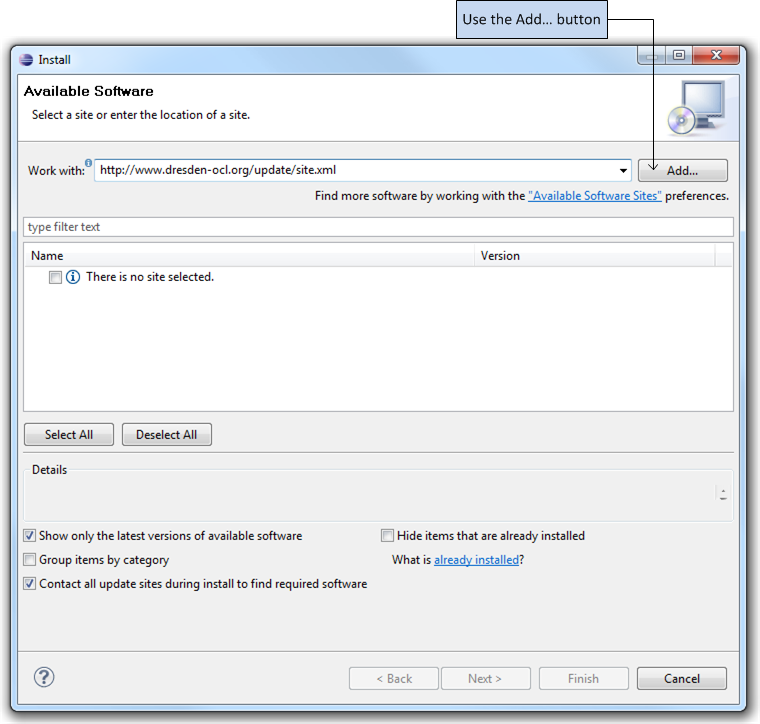
\includegraphics[width=0.8\linewidth]{figures/introduction/updateSite01}
	\caption{Adding an Eclipse Update Site (Step 1).}
	\label{pic:intro:updateSite01}

  \vspace{2.0em}
  
	\centering
	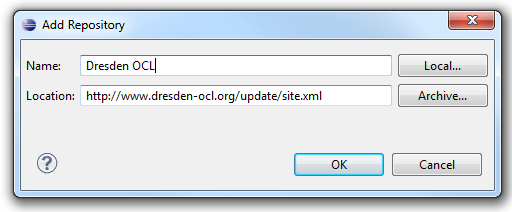
\includegraphics[width=0.6\linewidth]{figures/introduction/updateSite02}
	\caption{Adding an Eclipse Update Site (Step 2).}
	\label{pic:intro:updateSite02}
\end{figure}

Now you can select the features of Dresden OCL which you want to install. 
Select them and click the \eclipse{Next >} button (cf. 
Fig.~\ref{pic:intro:updateSite03}). An overview on all features of 
Dresden OCL can be found in Table~\ref{tab:plugins} in the appendix of 
this manual. Follow the wizard and agree with the user license. Then Dresden OCL
will be installed. Afterwards, you should restart your Eclipse application to 
finish the installation.

\begin{figure}[t]
	\centering
	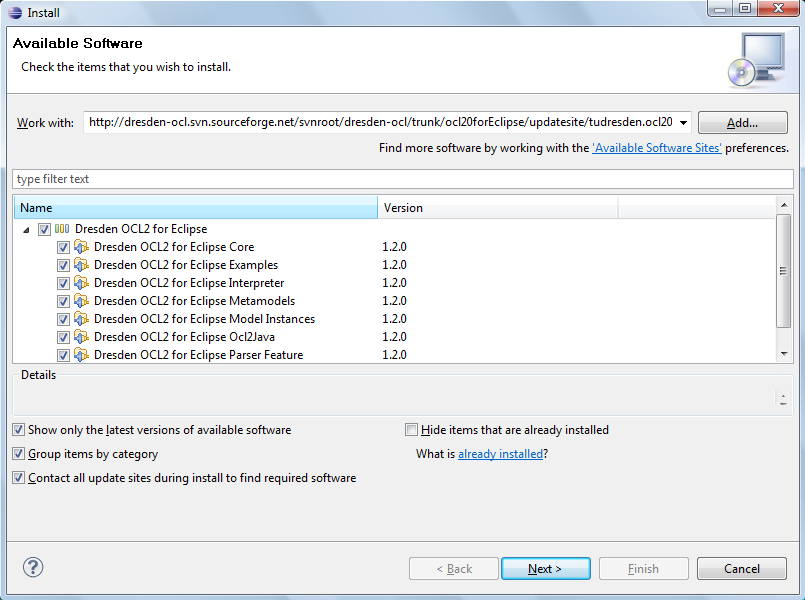
\includegraphics[width=1.0\linewidth]{figures/introduction/updateSite03}
	\caption{Selecting features of Dresden OCL.}
	\label{pic:intro:updateSite03}
\end{figure}
	
	
\subsection{Importing Dresden OCL from the SVN}

To use Dresden OCL by checking out the source code from the \acs{SVN} you
need to install an \acs{SVN} client. In the following the 
\keyword{Eclipse Subversive} plug-in is used.

After installing Eclipse Subversive, a new \keyword{Eclispe Perspective} 
providing access to \acs{SVN} should exist. The perspective can be opened via 
the menu \eclipse{Window > Open Perpective > Other... > SVN Repository
Exploring}. In the view \eclipse{\acs{SVN} Repositories} you can add a new 
repository using the \acs{URL} 
\url{http://svn-st.inf.tu-dresden.de/svn/dresdenocl/} (cf. 
Fig.~\ref{pic:intro:svn01}).

\begin{figure}[!b]
	\centering
	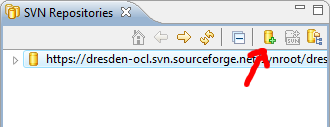
\includegraphics[width=0.4\linewidth]{figures/introduction/svn01}
	\caption{Adding an SVN repository.}
	\label{pic:intro:svn01}
\end{figure}

After clicking the \eclipse{Finish} button, the \acs{SVN} repository root should 
be visible in the \eclipse{\acs{SVN} Repositories} view. To checkout the
plug-ins, you have to select them in the repository directory 
\reference{trunk/ocl20\-for\-Eclipse/eclipse} and use the \eclipse{Checkout...} 
function in the context menu (cf. Fig.~\ref{pic:intro:svn02}).
	
\begin{figure}[!t]
	\centering
	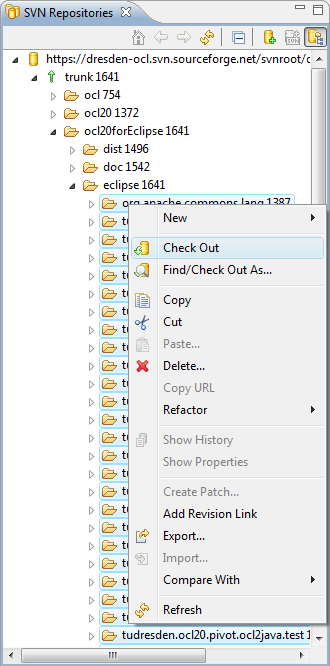
\includegraphics[width=0.4\linewidth]{figures/introduction/svn02}
	\caption{Checkout of Dresden OCL's plug-in projects.}
	\label{pic:intro:svn02}
\end{figure}


\subsection{Problems While Installing Dresden OCL}

Dresden OCL required some other plugins as a prerequesite for its installation. Unfortunately,
the mechanism to declare these dependencies automatically does not work with all installations of
Eclipse well. If during the installation of Dresden OCL problems such as unresolved dependencies occur,
you have to declare these dependent update sites manually.

Open the p2 update manager by the menu option \emph{Help -> Install New Software\ldots}.

Enter the following update sites and confirm each site by pressing the \emph{Add} button:

\begin{itemize}
  \item \url{http://www.emftext.org/update/}
  \item \url{http://download.eclipse.org/tools/ajdt/42/dev/update/}
\end{itemize}

Afterwards, the problem with unresolved dependencies should not occur anymore.


\subsection{Building the OCL2 Parser}
The new Dresden OCL parser/editor is partially written in Scala. In order
to build the sources of the parser without having to have the \reference{Scala
IDE} installed, Dresden OCL comes with various \keyword{Ant} scripts that
compile the Scala code to byte code.

After a checkout, the build script should be called automatically. Be aware that
the compilation might take a while to finish. If other projects that depend on
the parser like the facade still do not compile correctly, try to perform a 
\keyword{refresh} on the plug-ins that contain Scala code.

If the \keyword{Ant} script is not invoked automatically, you can call it either
be cleaning the
\reference{tudresden\linebreak[0].ocl\-20\linebreak[0].pivot.language.ocl.staticsemantics}
plug-in or by running the \keyword{Ant} task \reference{clean all} of the same plug-in.

You have to run the \keyword{ANT} scripts in the same 
\keyword{JRE} as Eclipse. Figures~\ref{pic:intro:parserbuild01} 
and~\ref{pic:intro:parserbuild02} show how to achieve this. If an error like 
``Unable to find javac compiler.'' occurs, you might be trying to run the
\keyword{Ant} script with a \keyword{\acl{JRE}} instead of a \keyword{\acs{JDK}}
(For errors like this one) use the \eclipse{Installed JREs...} button in the
same window to select a \acs{JDK} instead.

If you want to make changes to the static semantics evaluation of the parser you
should consider installing the \emph{Scala IDE} from 
\url{http://www.scala-lang.org/scala-eclipse-plugin}. Be aware that the Scala
code is version 2.7.7 which is not compatible with Scala 2.8 and therefore you
cannot use the current \emph{Scala IDE} which supports only Scala 2.8. 

In order to use the Scala compiler of the IDE, you have to go to the
\eclipse{Properties} of each Scala plug-in, select the tab \eclipse{Builders},
check the \eclipse{Scala Builder} and possibly uncheck the \keyword{Ant} script
for building.

\begin{figure}[p]
	\centering
	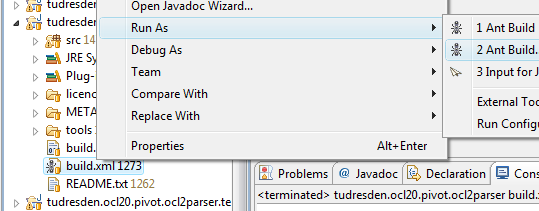
\includegraphics[width=0.8\linewidth]{figures/introduction/parserbuild01}
	\caption{Executing the OCL2 Parser build script.}
	\label{pic:intro:parserbuild01}

  \vspace{4.0em}

	\centering
	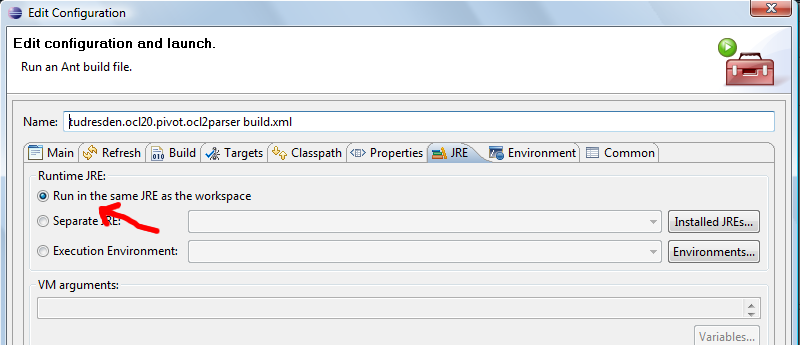
\includegraphics[width=0.8\linewidth]{figures/introduction/parserbuild02}
	\caption{Settings of the JRE for the Ant build script.}
	\label{pic:intro:parserbuild02}

  \vspace{4.0em}

	\centering
	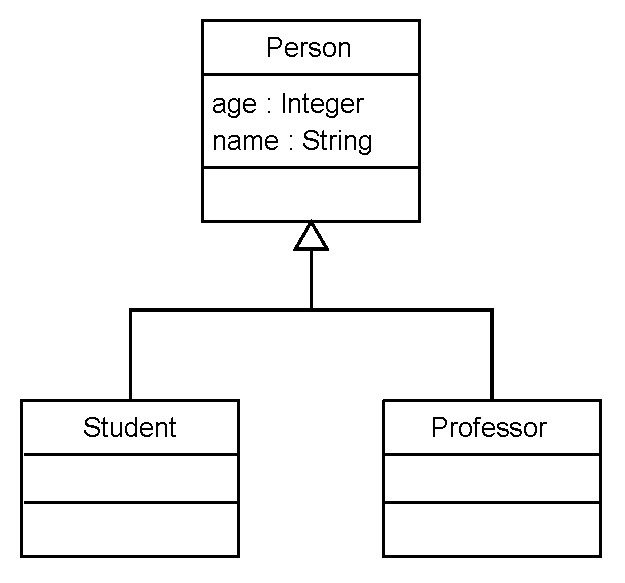
\includegraphics[width=0.5\linewidth]{figures/examples/simple01}
	\caption{A class diagram describing the Simple Example model.}
	\label{pic:examples:simple01}
\end{figure}


\section{Loading Models, Model Instances and Constraints}

If you installed the Dresden OCL using the market place client or update site,
you can execute the toolkit within your Eclipse distribution. If you imported
the Toolkit as source code plug-ins into an Eclipse workspace, you have to start a 
new Eclipse instance. You can start a new instance via the menu \eclipse{Run >
Run As > Eclipse Application}. If the menu \eclipse{Eclipse Application} is not 
available or disabled you need to select one of the plug-ins of the toolkit in
the \eclipse{Package Explorer} first.


\subsection{The Simple Example}
\label{intro:simpleExample}

The use of Dresden OCL is explained using the \keyword{Simple Example} 
which is located in the plug-in 
\reference{tudresden.ocl20.pivot.examples.\linebreak[0]simple}. 
Figure~\ref{pic:examples:simple01} shows a class diagram of the Simple Example.

Dresden OCL provides more examples than the Simple Example. The different 
examples use different metamodels which is possible with the \textit{Pivot
Model} architecture of the Toolkit. An overview on all examples provided 
with Dresden OCL is listed in Table~\ref{tab:examples} in the appendix of
this manual. The Simple Example can be used with two different metamodels. 
These are \keyword{\acs{UML}~2} (based on \keyword{\acs{Eclipse MDT} 
\acs{UML}}) and \keyword{Java}.


\subsection{Dresden OCL Perspective}

Dresden OCL provides its own perspective within Eclipse that contains all views
and editors provided with Dresden OCL. To ease the work with Dresden OCL, you
should now switch to the Dresden OCL perspective. Select the menu option
\eclipse{Window -> Open Perspective -> Other \ldots} and select the perspective
\eclipse{Dresden OCL} (cf. Fig.~\ref{pic:introduction:perspective}).
	
\begin{figure}[!t]
	\centering
	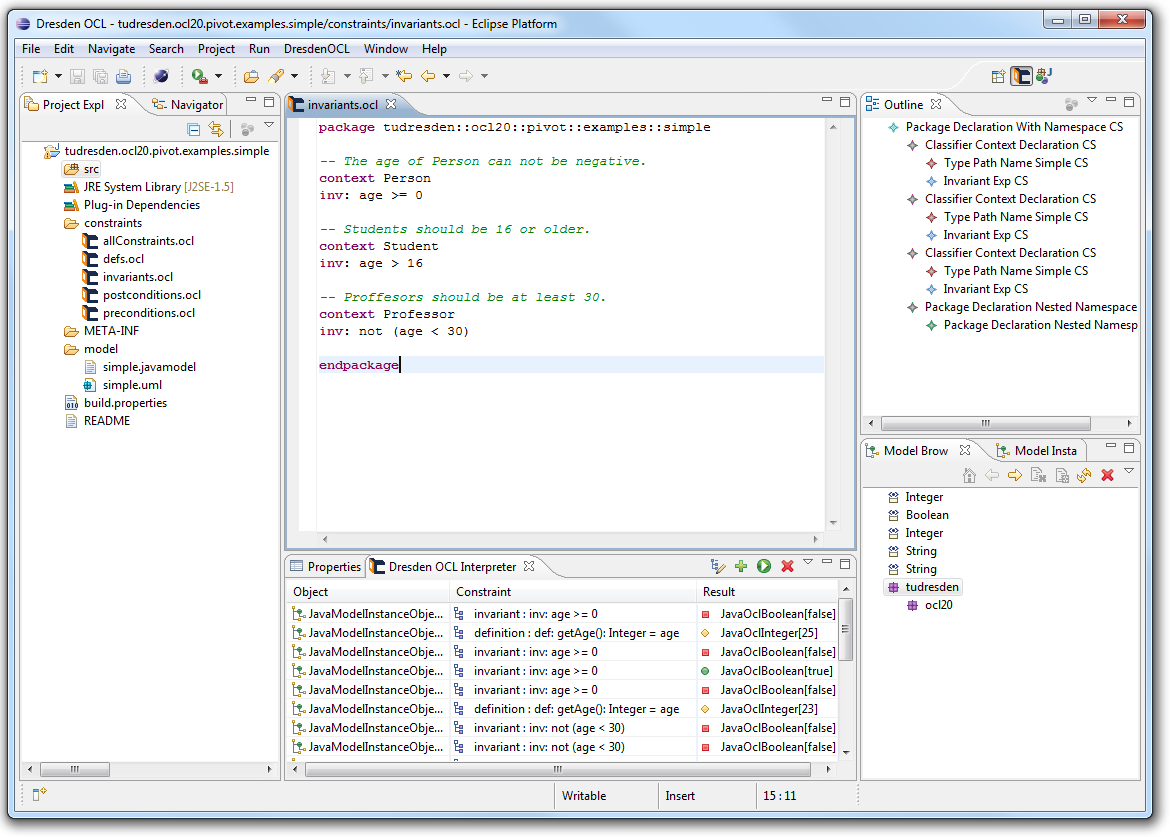
\includegraphics[width=1.0\linewidth]{figures/introduction/perspective}
	\caption{The Dresden OCL Perspective.}
	\label{pic:introduction:perspective}
\end{figure}

On the left hand side the perspective contains the \eclipse{Project Explorer} of
Eclipse to manage different projects. The right hand side contains the
\eclipse{Outline View} for opened \acs{OCL} files. Below, the \eclipse{Model
Browser} and \eclipse{Model Instance Browser} of Dresden OCL allow to explore models and
instances imported into Dresden OCL. At the bottom of the perspective the
\eclipse{OCL Intepreter} is located. The center of the perspective contains the
\eclipse{OCL Editor} of Dresden OCL that allows to edit and parse \acs{OCL}
files for an opened model. How to use the tools provided with Dresden OCL is explained in
the following.


\subsection{Loading a Model}
	
For this tutorial you first have to load a model into Dresden OCL. To ease the
use of the Simple Example project, this project should be imported into the  
\keyword{Workspace} first. Select the menu option \emph{File -> New ->
Other} and select the option \emph{Dresden OCL Examples -> Simple Example}
within the new opened window (cf. Fig~\ref{pic:intro:importexample01}). Click
the \emph{Finish} button to import the project into your workspace. Afterwards, the workspace should contain the Simple
Example project as shown in Figure~\ref{pic:introduction:perspective}, left hand
side.

\begin{figure}[!t]
	\centering
	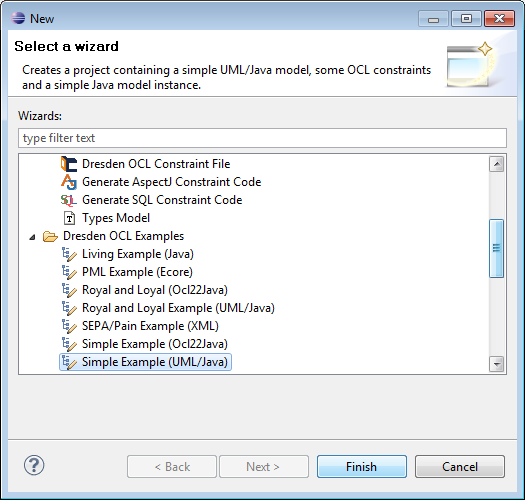
\includegraphics[width=0.8\linewidth]{figures/introduction/importexample01}
	\caption{Importing the Simple Example project.}
	\label{pic:intro:importexample01}
\end{figure}

Now you can import the model into Dresden OCL. Select the
\reference{model/simple.uml} file in the \eclipse{Project Explorer} and open the
context menu (right mouse click). Select the menu option
\eclipse{Dresden OCL > Load Model} (cf. Fig.~\ref{pic:intro:loadmodel00}). In
the opened wizard you have to select the metamodel \acs{UML}2 and click the
\eclipse{Finish} button (cf. Fig.~\ref{pic:intro:loadmodel01}).

Figure~\ref{pic:intro:loadmodel02} shows the imported Simple Example model,
which uses \acs{UML}2 as its meta-model. Via the menu button of the \eclipse{Model 
Browser} (the little triangle in the right top corner) you can switch between 
different models imported into Dresden OCL (cf.  
Fig.~\ref{pic:intro:loadmodel03}). With the two circled arrows icon you can
reload a model into Dresden OCL, with the red \emph{X} you can close the
currently selected model.
	
\begin{figure}[!p]
	\centering
	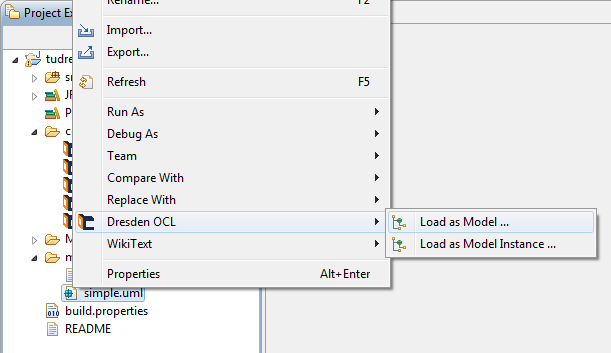
\includegraphics[width=1.0\linewidth]{figures/introduction/loadmodel00}
	\caption{Loading a Model.}
	\label{pic:intro:loadmodel00}
	
  \vspace{6.0em}
	\centering
	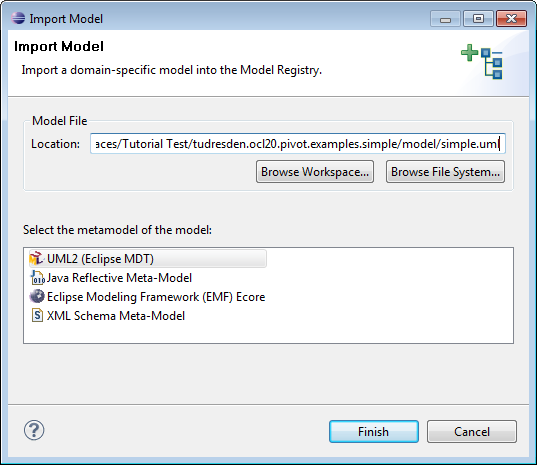
\includegraphics[width=0.7\linewidth]{figures/introduction/loadmodel01}
	\caption{Loading a Model.}
	\label{pic:intro:loadmodel01}
\end{figure}
	
\begin{figure}[!p]
	\centering
	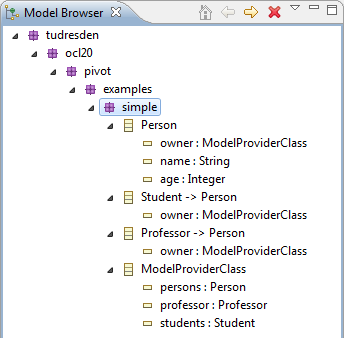
\includegraphics[width=0.4\linewidth]{figures/introduction/loadmodel02}
	\caption{The Simple Example model within the Model Browser.}
	\label{pic:intro:loadmodel02}
	
	\vspace{6.0em}

	\centering
	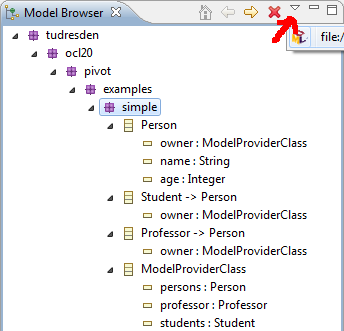
\includegraphics[width=0.4\linewidth]{figures/introduction/loadmodel03}
	\caption{You can switch between different Models using the little triangle.}
	\label{pic:intro:loadmodel03}
	
\end{figure}

	
\subsection{Loading a Model Instance}
\label{intro:loadModel}

After loading a model, you can load an instance of this model using another 
wizard. The model instance is required to interpret \acs{OCL} constraints on
elements instantiating the classes described in the opened model. Which kinds
of model instances are supported in Dresden OCL is documented in
Section~\ref{sect:info:modelinstances}. 
Since the Simple Example provides a Java model instance, we now have to select a
\code{*.java} or \code{*.class} file. Select the file
\reference{src/tudresden/ocl20/\linebreak[0]pivot/examples/\linebreak[0]sim\-ple/\linebreak[0]in\-stance/\linebreak[0]Mo\-del\-InstanceProviderClass\linebreak[0].java}
of the Simple Example in the \eclipse{Project Explorer}. Open the context menu 
and select the menu option \eclipse{Dresden OCL > Load Model Instance} (cf.
Fig.~\ref{pic:intro:loadInstance00}).
In the opened wizard you have to select a model for which the model instance 
shall be loaded and the type of model instance you want to load (cf.
Fig.~\ref{pic:intro:loadInstance01}). Select the \keyword{Java Instance} type
and click the \eclipse{Finish} button.

\begin{figure}[!p]
	\centering
	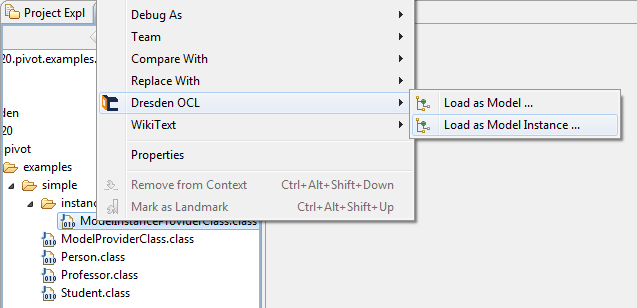
\includegraphics[width=0.7\linewidth]{figures/introduction/loadinstance00}
	\caption{Loading a Simple Model Instance.}
	\label{pic:intro:loadInstance00}

  	\vspace{6.0em}
  
	\centering
	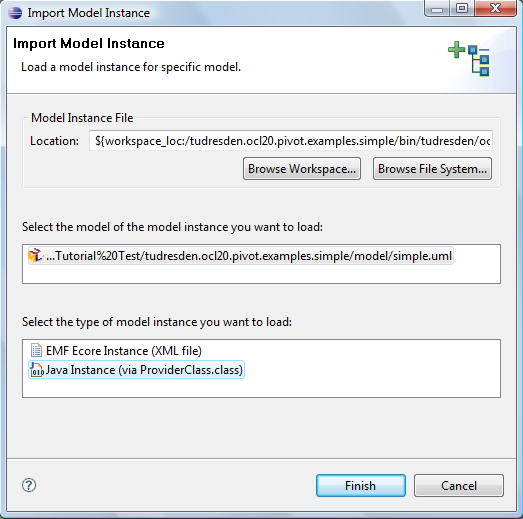
\includegraphics[width=0.7\linewidth]{figures/introduction/loadinstance01}
	\caption{Loading a Simple Model Instance.}
	\label{pic:intro:loadInstance01}
\end{figure}

Figure~\ref{pic:intro:loadInstance02} shows the imported model instance. Like
in the model browser you can switch between different model instances and you 
can close selected instances. Note that the \eclipse{Model Instance Browser} 
only shows the model instances of the model actually selected in the model 
browser. By switching the model in the model browser, you also switch the pool 
of model instances available in the model instance browser.

\begin{figure}[!p]
	\centering
	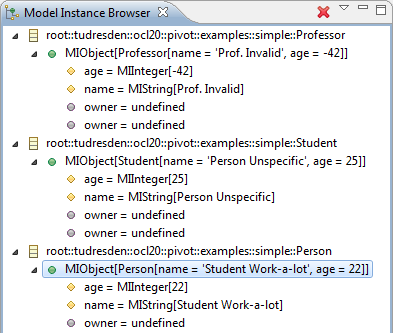
\includegraphics[width=0.6\linewidth]{figures/introduction/loadinstance02}
	\caption{A simple model instance in the Model Instance Browser.}
	\label{pic:intro:loadInstance02}

	\vspace{4.0em}
	
	\centering
	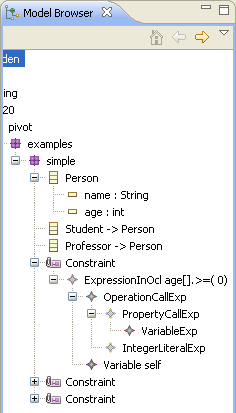
\includegraphics[width=0.4\linewidth]{figures/introduction/loadconstraints02}
	\caption{Parsed expressions and the model in the Model Browser.}
	\label{pic:intro:loadconstraints02}
\end{figure}
	
	
\subsection{Parsing OCL Expressions}
\label{intro:oclEditor}
Any file with the file extension \texttt{.ocl} can be opened with the
\keyword{Dresden OCL Editor}. Once opened, syntactic checks are performed
to analyse whether the given file contains valid \acs{OCL} code. If currently
there is no active model selected in the \eclipse{Model Browser}, the editor
will fail to perform the static semantics analysis and will yield that there is
no active model. You can load a model and then re-parse the \acs{OCL} file by
changing the \acs{OCL} file (e.g., by introducing and immediately deleting a
whitespace character).

The editor/parser will automatically add parsed constraints to the
model as well as \keyword{definitions} to the appropriate
classes. You can inspect the changes on the model in the \eclipse{Model
Browser}. Note that the \keyword{definitions} and constraints are not added to
your model -- they belong to the view of Dresden OCL on the model. The result
can be seen in Figure~\ref{pic:intro:loadconstraints02}. You also can remove
parsed constraints from the model which is shown in
Figure~\ref{pic:intro:loadconstraints03}.

\begin{figure}[t]
	\centering
	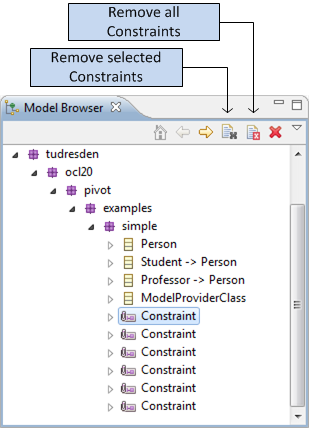
\includegraphics[width=0.4\linewidth]{figures/introduction/loadconstraints03}
	\caption{How to remove Constraints from a Model again.}
	\label{pic:intro:loadconstraints03}
\end{figure}


\subsection{Referencing the constrained Model}

The architecture of Dresden OCL requires that a model must always be imported before
a constraint file can be parsed correctly. Thus, if a constraint file is opened before
its model has been loaded, its complete contend will be marked as erroneous, as the
OCL parser is not able to resolved the referenced files.

To avoid this situation, an annotation can be added to an OCL file that references to
the constraint model specifying a relative path to the model file. The annotation must
be included in a comment at the top of the OCL file consisting of the pattern
\texttt{@model{<path>}} (e.g., for the constraint files of the simple example, the annotation
\texttt{@model{../model/simple.uml}} should work).


\subsection{Refactorings for Dresden OCL}

Dresden OCL can be extended with support for OCL refactorings to ease and improve OCL editing.
How refactorings can be installed and used in Dresden OCL is shortly explained in the following.

\subsubsection{Installation of Refactorings for Dresden OCL}

\begin{itemize}
  \item Install Refactory from the following URL: \url{http://www.emftext.org/update/}.
  \item Install the Refactoring for Dresden OCL feature from: 
  \url{http://www.modelrefactoring.org/DresdenOCLRefactoring/} 
\end{itemize}

\subsubsection{Usage of OCL Refactorings}

After installing the refactoring support, refactorings can simply be performed by selecting
an element in the OCL editor, opening the context menu and select the respective refactoring
(e.g., you can extract a variable as shwon in Fig.~\ref{pic:intro:refactoring01}--\ref{pic:intro:refactoring03}).

\begin{figure}
	\centering
	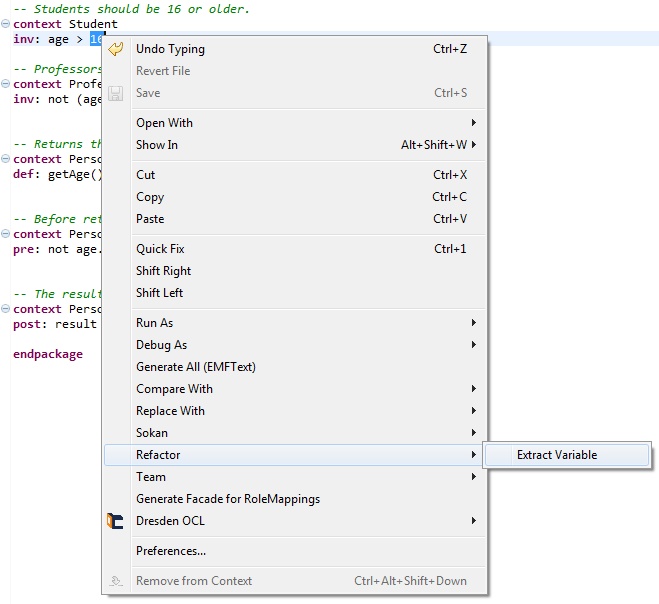
\includegraphics[width=0.35\linewidth]{figures/introduction/refactoring01.png}
	\caption{Extracting a variable: issue the refactoring.}
	\label{pic:intro:refactoring01}

	\vspace{2.0em}
	
	\centering
	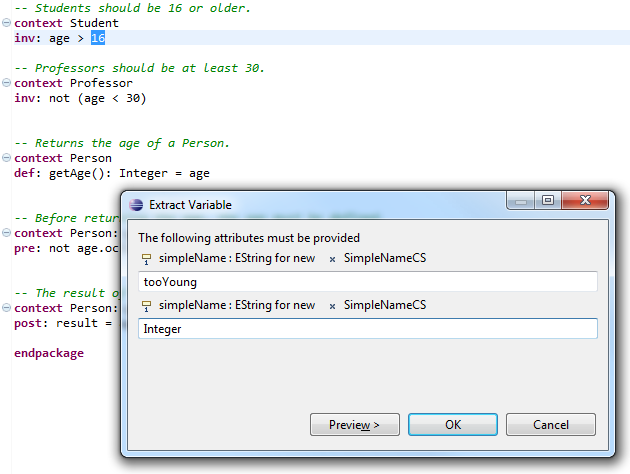
\includegraphics[width=0.8\linewidth]{figures/introduction/refactoring02.png}
	\caption{Extracting a variable: enter parameters.}
	\label{pic:intro:refactoring02}

	\vspace{2.0em}

	\centering
	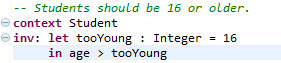
\includegraphics[width=0.35\linewidth]{figures/introduction/refactoring03.png}
	\caption{Extracting a variable: the result.}
	\label{pic:intro:refactoring03}
\end{figure}
	

\section{Possible Use Cases of Dresden OCL using different Models and Model
Instances}
\label{sec:usecases}

Dresden \acs{OCL} can be used in the context of different kind of models and
instances and even at different modeling layers. This section tries to name some 
prominent examples for possible use cases of Dresden \acs{OCL} w.r.t.
different kinds of models and instances. Readers who are not interested in
these details are encouraged to skip this section.

In general, Dresden \acs{OCL} supports the use of \acs{OCL} at two different 
levels: First, \acs{OCL} constraints can be defined on a metamodel and evaluated
on instances of this metamodel (i.e., models). In this context,
\acs{OCL} constraints are often called \emph{\acf{WFRs}}. Second, \acs{OCL}
constraints can be defined on a model and evaluated on instances of this model
(i.e., runtime objects or data). These constraints are often called
\emph{\acf{BRs}}. Examples for both use cases are shown in
Table~\ref{tab:usecases} and shortly explained in the following.

\begin{table}[!t]
\begin{tabular}{|p{7cm}p{7cm}|}
  \hline
  \textbf{WFR Specification and Evaluation} & \\
  \hline
  EMF/Ecore-based model,\newline e.g., \texttt{mydsl.ecore} &
  EMF/Ecore-based instance (model),\newline e.g., \texttt{model01.mydsl} \\
  \hline
  UML metamodel,\newline \texttt{uml.ecore} of MDT/UML &
  UML instance (model),\newline e.g., \texttt{model01.uml} \\
  \hline
  \hline
  \textbf{BR Specification and Evaluation} & \\
  \hline
  UML-based model,\newline e.g., \texttt{model01.uml} &
  Java-based instance (runtime objects),\newline e.g., \texttt{Instance01.java}
  \\
  \hline
  Java classes,\newline e.g., \texttt{Model01.java} &
  Java-based instance (runtime objects),\newline e.g., \texttt{Instance01.java}
  \\
  \hline
  XML Schema (\acs{XSD}),\newline e.g., \texttt{mySchema.xsd} &
  XML instance (data),\newline e.g., \texttt{Instance01.xml} \\
  \hline
\end{tabular}
\caption{Different possible use cases of Dresden OCL.}
\label{tab:usecases}
\end{table}


\subsection{Use Cases of Dresden OCL for Well-Formedness Rules}

Dresden \acs{OCL} supports different scenarios, where \acs{OCL} rules can be
specified on metamodels as \acs{WFRs}. The mose prominent scenarios are shortly
explained below.

\subsubsection{WFRs for EMF/Ecore Models} 
\acs{EMF}/Ecore is often used as a metamodeling language to develop \acl{DSL}s
(\acs{DSL}s). To specify \acs{OCL} constraints on an Ecore-based metamodel, you
import the model file (e.g., \texttt{mydsl.ecore}) as a model into Dresden
\acs{OCL} using the model importer for \acs{EMF}/Ecore-based models. Afterwards,
you can specify \acs{OCL} constraints using the \acs{OCL} parser/editor of
Dresden \acs{OCL}. You can import istances of your \acs{DSL} into Dresden
\acs{OCL} using the model instance importer for \acs{EMF}/Ecore-based instances
(e.g., \texttt{model01.mydsl}) to interpret the specified constraints on them.

\subsubsection{WFRs for the UML Metamodel}
Another common use case is the specification of \acs{OCL} constraints on the
\acs{UML} metamodel and their evaluation for instances of the metamodel (i.e.,
\acs{UML} models). You can do this by importing the \acs{EMF}/Ecore-based
\acs{UML}-metamodel of the Eclipse \acf{MDT}. You can find the required
\texttt{uml.ecore} within the Eclipse plug-in \texttt{org.eclipse.uml.uml} of
Eclipse MDT. Please note, when importing this metamodel into Dresden \acs{OCL},
you have to import it using the \acs{EMF}/Ecore model importer and not a
\acs{UML} model importer (since the \acs{UML} metamodel was modelled in \acs{EMF})!
Afterwards, you can import a \acs{UML} model as an instance of the metamodel to
evaluate constraints on it (e.g., \texttt{model.uml}). Again, you have use
the \acs{EMF}/Ecore model instance importer.


\subsection{Use Case of Dresden OCL for Busines Rules}

Besides the evaluation of \acs{WFRs}, multiple use cases for the evaluation of
\acf{BRs} are supported and explained below.

\subsubsection{BRs for UML models}
A common use case is the definition of \acs{OCL} constraints on a \acs{UML}
model (e.g., \texttt{model01.uml}), typically containing a class model. You can
import \acs{UML} class models into Dresden \acs{OCL} using the corresponding
model importer. For \acs{OCL} evaluation a
possible model instance is a set of runtime objects by using a Java class and
the Java model instance importer (e.g., \texttt{Instance01.java}). Details how
a Java class usable as a Java model instance must be implemented are documented
in Section~\ref{subsec:javaInstance}.

\subsubsection{BRs for Java Classes}
Another possible use case is the use of a set of Java classes as a model for
\acs{OCL} constraint specification (e.g., \texttt{Model01.java}). A Java class
can be imported as a model using the Java model importer. Details how the class
is imported as a model are documented in Section~\ref{subsec:javaModel}. Again,
a typical model istance would be a set of Java objects as mentioned above
(e.g., \texttt{Instance01.java}).

\subsubsection{BRs for XML Schemata}
Dresden \acs{OCL} supports the definition of \acs{OCL} rules on \acl{XSD}s
(\acs{XSD}s) as well (e.g., \texttt{mySchema.xsd}) using the \acs{XSD} model
importer. Obviously an \acs{XML} file would be an appropriate model instance,
using the \acs{XML} model instance importer (e.g., \texttt{Instance01.xml}).


\subsection{Further Use Cases}

Of course, the use cases presented above are not a complete list of all possible
use cases. Theoretically, every supported type of model importer can be combined
with every type of model instances. And besides, you can even define your own
importers for further use cases, if necessary. How to adapt Dresden \acs{OCL} to
other types of models and instances is documented in the
Chapters~\ref{chapter:pivotModelAdaptation}
and~\ref{chapter:modelInstanceTypeAdaptation}.



\section{Summary} 

This chapter described how to use Dresden OCL. It was explained how to 
install the plug-ins of Dresden OCL. Afterwards, the import of models,
model instances and \acs{OCL} constraints into Dresden OCL was explained.

Now, the imported models can be used with the tools provided by Dresden OCL. For
example you can use the \keyword{OCL Interpreter} to interpret \acs{OCL} 
constraints for a given model and model instance (as explained in 
Chapter~\ref{chapter:interpretation}) or you can use the \keyword{OCL22Java
Code Generator} to generate \keyword{AspectJ} code for a loaded model and 
\acs{OCL} constraints (as explained in Chapter~\ref{chapter:codeGeneration}).
How the \keyword{OCL2SQL Code Generator} can be used to generated SQL schema and
integretiy views is documented in Chapter~\ref{chapter:ocl2sql}.

If you do not want to use Eclipse, but still want to interpret OCL constraints 
or generate AspectJ code, you can use Dresden OCL as a stand-alone library
outside of Eclipse. A detailed description on how to do this is given in 
Chapter~\ref{chapter:standalone}.
\chapter{OCL Interpretation}
\label{chapter:interpretation}

\begin{flushright}
\textit{Chapter written by Claas Wilke}
\end{flushright}

This chapter describes how the \acs{OCL} Interpreter provided with Dresden OCL 
can be used. How to install and run Dresden OCL and how 
to load models and OCL constraints was explained in 
Chapter~\ref{chapter:introduction}. If you are not familiar with such basic uses
of Dresden OCL, read Chapter~\ref{chapter:introduction} first.



\section{The Simple Example}

This chapter uses the \keyword{Simple Example} which is provided with 
\acl{DOT4Eclipse} located in the plug-in 
\reference{tudresden.ocl20.pivot.examples.\linebreak[0]simple}. An overview over
all examples provided with \acl{DOT4Eclipse} can be found in 
Table~\ref{tab:examples} in the appendix of this manual. An introduction into
the Simple Example can be found in Section~\ref{intro:simpleExample}. The model 
of the example defines three classes: The class \model{Person} has the 
attributes \model{age} and \model{name}. Two subclasses of \model{Person} are 
defined, \model{Student} and \model{Professor}.

To run this tutorial, import the Simple Example as explained in
Section~\ref{intro:simpleExample}. Figure~\ref{pic:example:simple02} shows the
\eclipse{Project Explorer} containing the imported project.

\begin{figure}[!t]
	\centering
	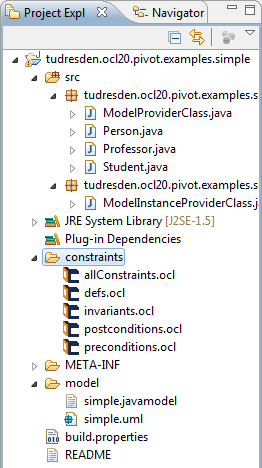
\includegraphics[width=0.5\linewidth]{figures/examples/simple02}
	\caption{The Project Explorer containing the Project which is required to run
	this Tutorial.}
	\label{pic:example:simple02}
\end{figure}
	
\begin{figure}[!t]
  \lstset{
    language=OCL
  }
  \begin{lstlisting}[caption={The Constraints contained in the Constraint File.}, captionpos=b, label=lst:interpret:allConstraints]
-- The age of Person can not be negative.
context Person
inv: age >= 0

-- Students should be 16 or older.
context Student
inv: age > 16

-- Proffesors should be at least 30.
context Professor
inv: not (age < 30)

-- Returns the age of a Person.
context Person
def: getAge(): Integer = age

-- Before returning the age, the age must be defined.
context Person::getAge()
pre: not age.oclIsUndefined()

-- The result of getAge must equal to the age of a Person.
context Person::getAge()
post: result = age
  \end{lstlisting}
\end{figure}

The project provides a model file that contains a class diagram (the model file 
is located at \model{model/simple.uml}) and the constraint file we want to
interpret (located at 
\model{constraints\linebreak[0]/\linebreak[0]all\-Con\-straints.ocl}). 
Listing~\ref{lst:interpret:allConstraints} shows the constraints defined in the
constraint file.

First, the constraint file defines three simple invariants that ensure that 
the \model{age} of every \model{Person} must always zero or greater than zero. 
Furthermore, the \model{age} of every \model{Student} must be greater than
\model{16} and the \model{age} of every \model{Professor} does not have to be
lesser than \model{30}.

In addition to that the constraint file contains a definition constraint that 
defines a new operation \model{getAge()} which returns the \model{age} of a 
\model{Person}. A precondition checks, that the \model{age} must be defined 
before it can be returned by the operation \model{getAge()}. And finally, a 
postcondition which checks, whether or not the result of the operation 
\model{getAge()} is the same as the \model{age} of the \model{Person}.



\section{Preparation of the Interpretation}

To prepare the interpretation we have to import the model 
\model{model/simple.uml} for which we want to interpret constraints into the
\eclipse{Model Browser}. We use the model import wizard of Dresden OCL to import
the model. This procedure is explained in Section~\ref{intro:loadModel}. 
Furthermore, we have to import a model instance for which the constraints shall 
be interpreted into the \eclipse{Model Instance Browser}. We use another import 
wizard to import the model instance 
\model{bin/tudresden/ocl20/pivot/\linebreak[0]exam\-ples/\linebreak[0]simple\linebreak[0]/\linebreak[0]ModelProviderClass.class}.
Finally, we have to open the constraint file 
\model{con\-straints/\linebreak[0]all\-Con\-straints\linebreak[0].ocl}
containing the constraints we want to interpret. Afterwards, the \eclipse{Model
Browser} should look like illustrated in Figure~\ref{pic:interpret:prepare01} 
and the \eclipse{Model Instance Browser} should look like shown in 
Figure~\ref{pic:interpret:prepare02}.

\begin{figure}[!p]
	\centering
	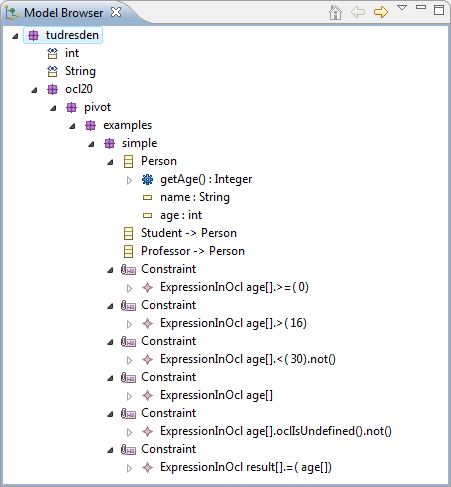
\includegraphics[width=0.6\linewidth]{figures/interpreter/prepare01}
	\caption{The Model Browser containing the Simple Model and its Constraints.}
	\label{pic:interpret:prepare01}

  \vspace{4.0em}
  
	\centering
	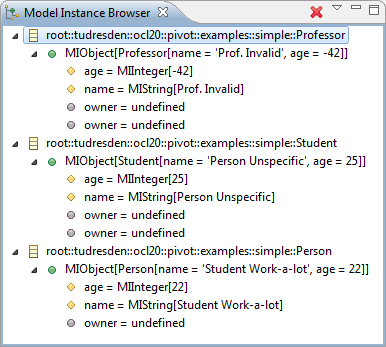
\includegraphics[width=0.6\linewidth]{figures/interpreter/prepare02}
	\caption{The Model Instance Browser containing the Simple Model Instance.}
	\label{pic:interpret:prepare02}
\end{figure}

The opened model instance contains three instances of the classes defined in the
Simple Example model. One instance of \model{Person}, one instance of 
\model{Student} and one instance of \model{Professor}. For these three instances
we now want to interpret the imported constraints.



\section{OCL Interpretation}

Now we can start the interpretation. To open the \acs{OCL} Interpreter we use 
the menu option \eclipse{Dresden OCL2 > Open OCL2 Interpreter}. The 
\eclipse{OCL Interpreter View} should now be visible (see 
Figure~\ref{pic:interpret:interpret01}).

By now, the \eclipse{OCL Interpreter View} does not contain any result. Besides
the results table, the view provides four buttons to control the \acs{OCL} 
Interpreter. The buttons are shown in Figure~\ref{pic:interpret:interpret02}. 
With the first button (from left to right) constraints can be prepared for 
interpretation. The second button can be used to add variables to the 
\keyword{Interpreter's Environment}. The third button provides the core 
functionality, it can be used to start the interpretation. And finally, the 
fourth button provides the possibility to delete all results from the 
\eclipse{OCL Interpreter View}. The functionality of the buttons will be 
explained below.

\begin{figure}[!p]
	\centering
	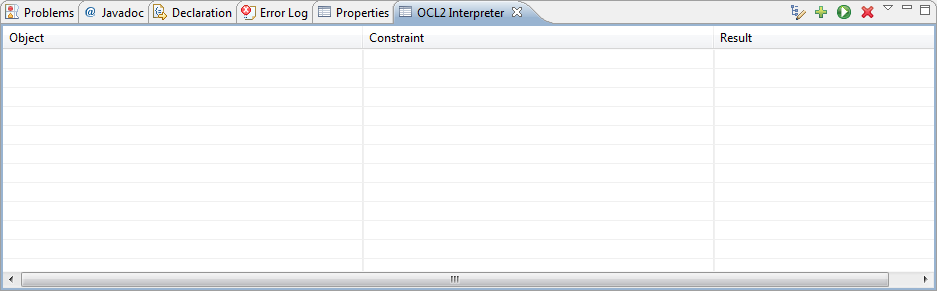
\includegraphics[width=1.0\linewidth]{figures/interpreter/interpret01}
	\caption{The OCL2 Interpreter View containing no results.}
	\label{pic:interpret:interpret01}

  \vspace{3.0em}
  
	\centering
	
\includegraphics[width=0.5\linewidth]{figures/interpreter/interpret02}
	\caption{The Buttons to Control the OCL2 Interpreter.}
	\label{pic:interpret:interpret02}

  \vspace{3.0em}

	\centering
	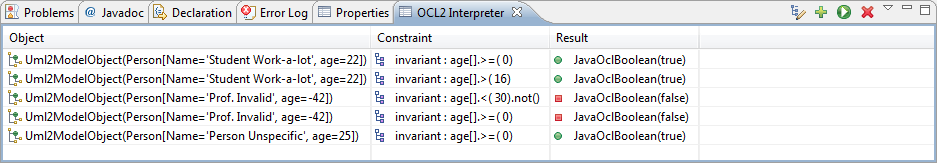
\includegraphics[width=1.0\linewidth]{figures/interpreter/interpret04}
	\caption{The results of the three Invariants for all Model Instance Elements.}
	\label{pic:interpret:interpret04}

  \vspace{3.0em}

	\centering
	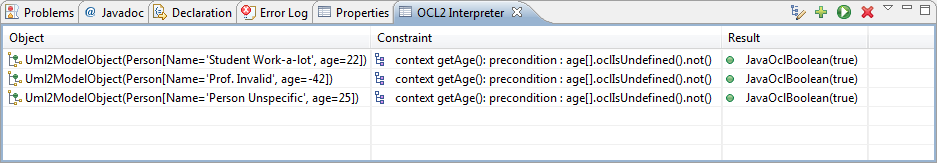
\includegraphics[width=1.0\linewidth]{figures/interpreter/interpret07}
	\caption{The results of the Definition for all Model Instance Elements.}
	\label{pic:interpret:interpret07}

\end{figure}


\subsection{Interpretation of Constraints}

To interpret constraints, we simple select them in the \eclipse{Model Browser} 
and push the button to interpret constraints (the third button from the left). 
First, we want to interpret the three invariants defining the range of the 
\model{age} of \model{Persons}, \model{Students} and \model{Professors}. We 
select them in the \eclipse{Model Browser} and push the \eclipse{Interpret} button.
The result of the interpretation is now shown in the \eclipse{\acs{OCL}
Interpreter View} (see Figure~\ref{pic:interpret:interpret04}).

The invariant \model{age >= 0} has been interpreted for all three model objects.
The results for the \model{Person} and the \model{Student} instances are 
\model{true} because their \model{age} is greater than zero. The result for the
\model{Professor} instance is \model{false} because its \model{age} is 
\model{-42}.

The two other invariants were only interpreted for the \model{Student} or the 
\model{Pro\-fessor} instance because their context is not the class 
\model{Person} but the class \model{Student} or the class \model{Professor}, 
respectively. Again, the \model{Student's} result is \model{true} and the 
\model{Professor's} result is \model{false}.

Besides invariants, \acs{OCL}~2.2 enables us to use \acs{OCL} expressions to
define new attributes and methods or to initialize attributes and methods. Such
\model{def}, \model{init} and \model{body} constraints cannot be interpreted to
\model{true} or \model{false}, because their result type has not to be 
\model{Boolean}. Furthermore, they can be used to alter the results of other 
constraints that shall be interpreted. The \model{allConstraints.ocl} file 
contains a definition constraint, which defines the method \model{getAge()} for 
the class \model{Person}. Now, we want to interpret this definition constraint. 
We select the constraint in the \eclipse{Model Browser} and push the \eclipse{Interpret} button.
The result of the interpretation is shown in 
Figure~\ref{pic:interpret:interpret07}. The interpretation finishes for all
three instances successfully because the attribute \model{age} has been set for 
all three instances.


\subsection{Adding Variables to the Environment}

When interpreting OCL constraints from the GUI, we have to add further context 
information to interpret some pre- and postconditions. For example, the 
postcondition contained in the constraint file compares the result of the 
method \model{getAge()} with the attribute \model{age} of the referenced 
\model{Person} instance. Therefore, \acs{OCL} provides the special variable 
\model{result} in postconditions which contains the result of the constrained 
method's execution. Using the \eclipse{\acs{OCL} Interpreter View} we cannot 
execute the method \model{getAge()} and store the result in the \model{result} 
variable. We can interpret the postcondition in a specific context which has to 
be prepared by hand only. We have to set the result variable manually.

If we interpret the postcondition constraint (the sixth and last constraint in 
the \eclipse{Model Browser}) without setting the \model{result} variable, the 
constraint results in a \model{undefined} result for all three model instances
(see Figure~\ref{pic:interpret:interpret08}).

To prepare the variable, we push the button to add new variables to the 
Interpreter Environment (the second button from the left) and a new window opens
which we can use to specify new variables. We enter the name \model{result}, 
select the variable type \model{Integer} and enter the value \model{25}. Then we
push the \eclipse{OK} button (see Figure~\ref{pic:interpret:interpret09}. The 
result variable has now been added to the Interpreter's Environment.

\begin{figure}[!p]
	\centering
	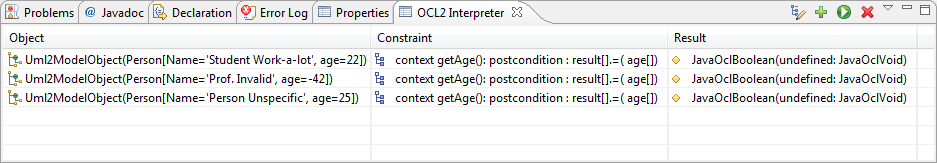
\includegraphics[width=1.0\linewidth]{figures/interpreter/interpret08}
	\caption{The results of the Postcondition without preparing the Result Variable.}
	\label{pic:interpret:interpret08}

  \vspace{3.0em}
	
	\centering
	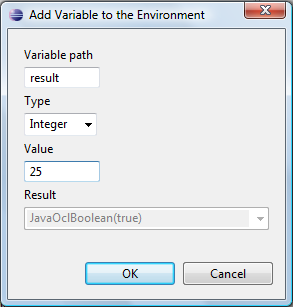
\includegraphics[width=0.5\linewidth]{figures/interpreter/interpret09}
	\caption{The Window to add new Variables to the Environment.}
	\label{pic:interpret:interpret09}

  \vspace{3.0em}
	
	\centering
	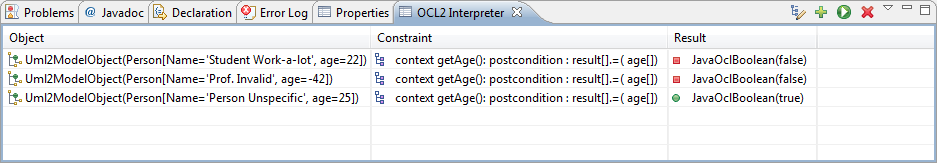
\includegraphics[width=1.0\linewidth]{figures/interpreter/interpret10}
	\caption{The Results of the Postcondition with Result Variable Preparation.}
	\label{pic:interpret:interpret10}
	
  \vspace{3.0em}

  \lstset{
    language=OCL
  }
  \begin{lstlisting}[caption={An example Precondition defined on an Operation with Argument.}, captionpos=b, label=lst:interpret:precondition]
-- arg01 must be defined.
context Person::setAge(arg01: Integer)
pre: not arg01.oclIsUndefined()
  \end{lstlisting}
\end{figure}

Now, we can interpret the postcondition again. The result is shown in 
Figure~\ref{pic:interpret:interpret10}. The results for the \model{Student} and
\model{Professor} instances are both \model{false} because their \model{age} 
attribute is not equal to \model{25} and thus the \model{result} value does not 
match to the \model{age} attribute. But the interpretation for the
\model{Person} instance succeeds because its \model{age} is \model{25}.

Other examples requiring manual addition of context information are pre- and
postconditions that are defined on operations containing arguments. 
Listing~\ref{lst:interpret:precondition} shows a precondition that is defined on
an operation \code{setAge(arg01)}. If the argument \code{arg01} is referred 
during interpretation, the interpreter has to know the value of the argument. 
Thus, we would have to add the value of \code{arg01} before the constraint's 
interpretation manually as shown for the \code{result} variable.


\subsection{Preparation of Constraints}

The interpretation of some postconditions requires a preparation of the 
Interpreter's environment before the operation defined in the context of the 
postcondition is invoked. Listing~\ref{lst:interpret:postcondition} shows such a
postcondition. The postcondition is defined on an operation 
\code{birthdayHappens()} that increments the \code{age} of a \code{Person}. The 
postcondition checks, whether the \code{age} was incremented or not. Thus, the 
Interpreter has to store the value of \code{age} before the operation 
\code{birthdayHappens()} is invoked. Therefore, the Interpreter View provides a 
button to prepare constraints (the first button from the left). If you want to 
interpret such postconditions, first select and prepare your constraint. The
value of \code{age@pre} is then stored in the Interpreter's environment. 
Then you can invoke your model instance's operation (which is quite 
complicate from the GUI). Afterwards you can interpret the postcondition.

\begin{figure}[!t]
  \lstset{
    language=OCL
  }
  \begin{lstlisting}[caption={An example Postcondition that must be prepared.}, captionpos=b, label=lst:interpret:postcondition]
-- age must be incremented by one.
context Person::birthdayHappens()
post: age = age@pre + 1
  \end{lstlisting}
\end{figure}

The preparation of postconditions is not that useful when interpreting 
constraints from the GUI of Dresden OCL because you cannot invoke your 
operations here to alter your model instance's state. Nevertheless, like the 
possibility to add variables to the Interpreter's environment you can prepare 
postconditions from the GUI. These operations are much more useful when using 
Dresden OCL via its API and using the \acs{OCL} Interpreter to check \acs{OCL} 
constraints during the runtime of other software. Then you can prepare
constraints before methods are invoked and check postconditions afterwards, 
e.g., by using \emph{\acf{AOP}}.



\section{Summary}
  
This chapter described how \acs{OCL} constraints can be interpreted using the 
\acs{OCL} Interpreter of Dresden OCL. The preparation and interpretation of 
constraints has been explained, the addition of new variables to the 
Interpreter Environment has been shown. Besides the use of the Interpreter via 
Dresden OCL's GUI, you can also invoke the Interpreter via Dresden OCL's 
\acs{API}. The easiest way to connect to Dresden OCL is via its \emph{Facade} 
providing interfaces for all services of Dresden OCL. How to use Dresden OCL's 
facade is documented in Chapter~\ref{chapter:integration}.

\chapter{AspectJ Code Generation}
\label{chapter:codeGeneration}

\begin{flushright}
\textit{Chapter written by Claas Wilke}
\end{flushright}

This Chapter describes how the Java Code Generator \keyword{OCL22Java} provided with \acl{DOT4Eclipse} can be used. A general introduction into \acl{DOT4Eclipse}  can be found in Chapter \ref{chapter:introduction}. A detailed documentation of the development of OCL22Java can be found in the Minor Thesis (Gro�er Beleg) of Claas Wilke \cite{GB:Wilke}.

In addition to the general Eclipse installation the \keyword{\acf{AJDT}} are required to execute the code generated with OCL22Java. The \acs{AJDT} plug-ins can be found at the \acs{AJDT} website \cite{WWW:AJDT}. 
  


\section{Code Generator Preparation}

This Chapter uses the \keyword{Simple Example} which is provided with \acl{DOT4Eclipse} and has been introduced in Subsection \ref{intro:simpleExample} To import the Simple Example into our Eclipse workspace we have to create a new Java project into our Workspace (here called \model{tudresden.ocl20.pivot.\linebreak[0]examp\-les.\linebreak[0]simple}) and use the import wizard \eclipse{General -> Archive File} to import the example provided as a \acs{JAR} archive. In the following window we select the directory were the \acs{JAR} file is located (eventually the \model{plugins} or \model{dropins} directory inside the Eclipse root folder). We select the archive \model{tudresden.ocl20.pivot.\linebreak[0]examples.simple.jar} and click the \eclipse{Finish} button (if you use a source code distribution of \acl{DOT4Eclipse} instead, you can simple import the project \model{tudresden.ocl20.pivot.examples.simple} using the import wizard \eclipse{General -> Existing Projects into Workspace}).

Next, we have to import a second project called \model{tudresden.ocl20.pivot.\linebreak[0]examples.simple.\linebreak[0]constraints}. We can use the same mechanism explained above, but instead of a Java project we now create an \keyword{AspectJ Project} before we import the archive file (if the wizard to create an AspectJ project is not available you have to install the \acs{AJDT} first). Figure \ref{pic:example:simple03} shows the \eclipse{Package Explorer} containing both imported projects.

\begin{figure}[!b]
	\centering
	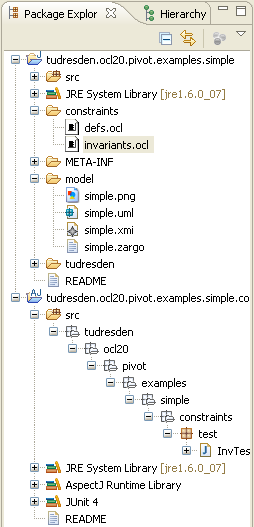
\includegraphics[width=0.5\linewidth]{figures/examples/simple03}
	\caption{The package explorer containing the two projects which are needed to run this tutorial.}
	\label{pic:example:simple03}
\end{figure}

\begin{figure}[!b]
	\centering
	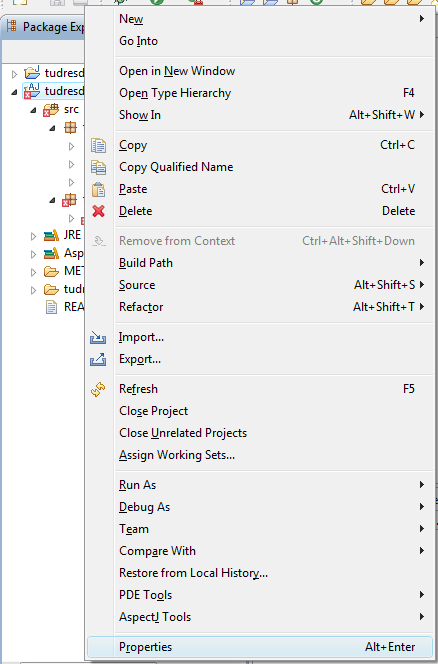
\includegraphics[width=0.8\linewidth]{figures/codegen/properties1}
	\caption{Selecting the properties settings.}
	\label{pic:codegen:properties1}
\end{figure}

After importing the second plug-in, we have to add the JUnit4 library to the project's build path. Right click on the project in the \eclipse{Package Explorer} and select the menu item \eclipse{Properties} (see Figure \ref{pic:codegen:properties1}). In the new opened window select the sub-menu \eclipse{Java Build Path -> Libraries} and click the button \eclipse{Add Library...} (see Figure \ref{pic:codegen:properties2}). In the following window select \eclipse{JUnit}, click \eclipse{Next}, select \eclipse{JUnit 4} and click \eclipse{Finish}. Click \eclipse{OK} to close the project's properties. The project should not contain any compile errors anymore.

\begin{figure}[!htbp]
	\centering
	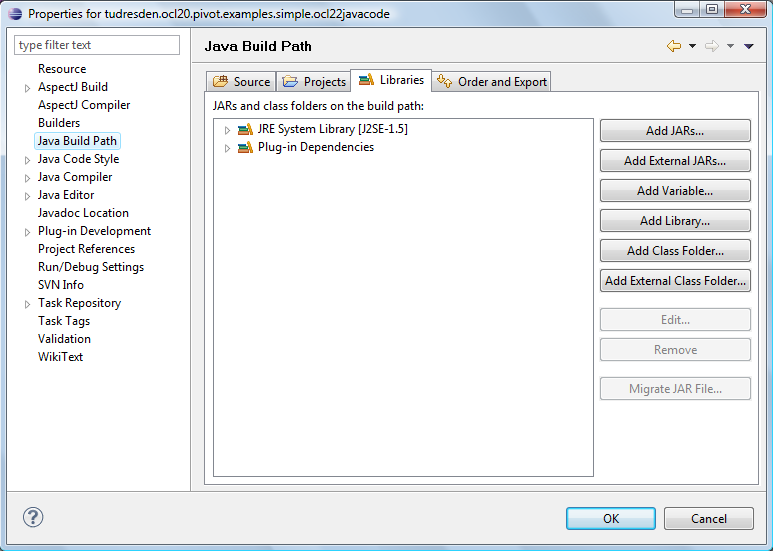
\includegraphics[width=1.0\linewidth]{figures/codegen/properties2}
	\caption{Adding a new library to the build path.}
	\label{pic:codegen:properties2}
\end{figure}

Now we have imported all files we need to run this tutorial. The first project provides a model file which contains the simple class diagram which has been explained in Subsection \ref{intro:simpleExample} (the model file is located at \model{model/simple.uml}) and the constraint file we want to generate code for (the constraint file is located at \model{constraints/invariants.ocl}). Listing \ref{lst:codegen:simpleInvariant} shows one invariant that is contained in the constraint file for which we want to generate code. The invariant declares, that the \model{age} of any \model{Person} must be greater or equal to zero at any time during the life cycle of the \model{Person}.

\lstset{
  language=OCL
}
\begin{lstlisting}[caption={A simple invariant.}, captionpos=b, label=lst:codegen:simpleInvariant, float]
-- The age of Person can not be negative.
context Person
inv: age >= 0
\end{lstlisting}

The second project provides the test class \model{src/tudresden.ocl20.pivot.examples.simple.\linebreak[0]con\-straints.\linebreak[0]InvTest.java} which contains a JUnit test case that checks, whether or not the mentioned constraint is enforced during run-time. The test case creates two \model{Persons} and tries to set their \model{age}. The \model{age} of the second \model{Person} is set to \model{-3} and thus the constraint is violated. The test case expects that a run-time exception is thrown, if the constraint is violated.

The code for the mentioned constraint has not been generated yet and thus the exception will not be thrown. We run the test case by right clicking on the Java class in the \eclipse{Package Explorer} and selecting the menu item \eclipse{Run as -> JUnit Test}. The test case fails because the exception is not thrown (see Figure \ref{pic:codegen:junit01}). To fulfill the test case we have to generate the ApsectJ code for the constraint which enforces the constraint's condition. How to generate such code will be explained in the following.

\begin{figure}[!htbp]
	\centering
	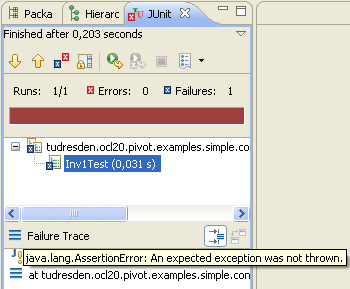
\includegraphics[width=0.6\linewidth]{figures/codegen/junit01}
	\caption{The result of the JUnit test case.}
	\label{pic:codegen:junit01}
\end{figure}



\section{Code Generation}

To prepare the code generation we have to import the model \model{model/simple.uml} into the \eclipse{Model Browser}. We use the import wizard for domain-specific models of the toolkit to import the model. This procedure is explained in the already mentioned introduction in Chapter \ref{chapter:introduction}. Afterwards, we have to import the constraint file \model{constraints/invariant.ocl} which is done by an import wizard again. After the importation, the \eclipse{Model Browser} should look like illustrated in Figure \ref{pic:codegen:modelBrowser}. Now we can start the code generation.

\begin{figure}[!htbp]
	\centering
	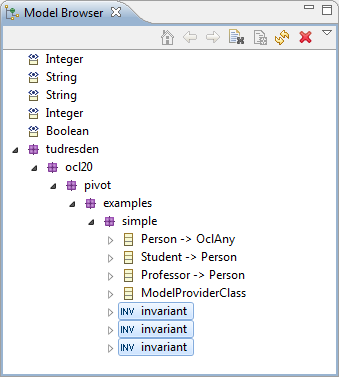
\includegraphics[width=0.6\linewidth]{figures/codegen/modelBrowser}
	\caption{The model browser containing the simple model and its constraints.}
	\label{pic:codegen:modelBrowser}
\end{figure}

To start the code generation we click on the menu item \eclipse{DresdenOCL} and select the item \eclipse{Generate AspectJ Constraint Code}. 


\newpage
\subsection{Selecting a Model}

A wizard opens and we have to select a model for code generation (see Figure \ref{pic:codegen:codegen01}). We select the \model{simple.uml} model and click the \eclipse{Next} button.

\begin{figure}[!b]
	\centering
	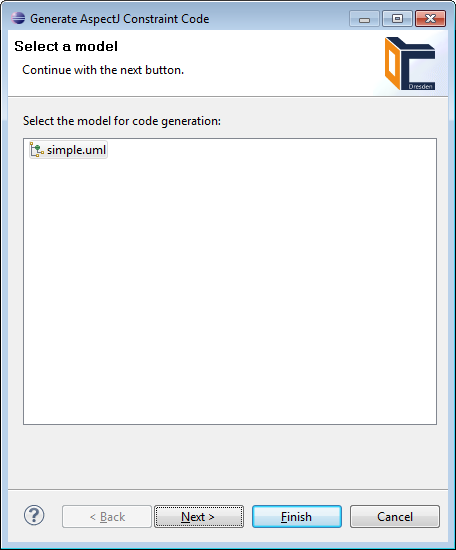
\includegraphics[width=1.0\linewidth]{figures/codegen/codegen01}
	\caption{The first step: Selecting a model for code generation.}
	\label{pic:codegen:codegen01}
\end{figure}


\newpage
\subsection{Selecting Constraints}

As a second step we have to select the constraints for that we want to generate code. We only select the constraint that enforces that the \model{age} of any \model{Person} must be equal to or greater than zero and click the \eclipse{Next} button (see Figure \ref{pic:codegen:codegen02}).

\begin{figure}[!b]
	\centering
	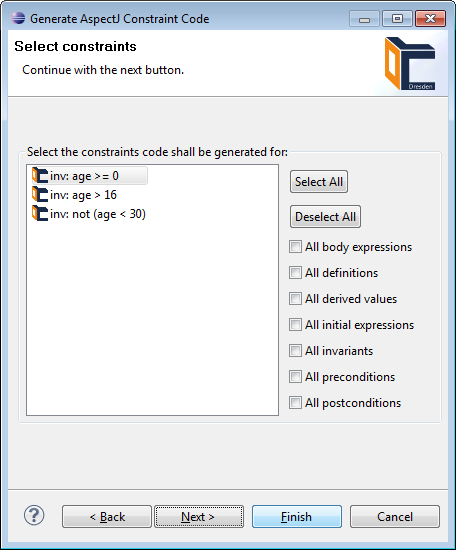
\includegraphics[width=1.0\linewidth]{figures/codegen/codegen02}
	\caption{The second step: Selecting constraints for code generation.}
	\label{pic:codegen:codegen02}
\end{figure}


\newpage
\subsection{Selecting a Target Directory}

Next, we have to select a target directory to that our code shall be generated. We select the source directory of our second project (which is \model{tudresden.\linebreak[0]ocl20.pivot.examples.simple.\linebreak[0]con\-straints/src}) (see Figure \ref{pic:codegen:codegen03}). Please note, that we select the source directory and not the package directory into which the code shall be generated! The code generator creates or uses contained package directories depending on the package structure of the selected constraint. Additionally we can specify a sub folder into that the constraint code shall be generated relatively to the package of the constrained class. By default this is a sub directory called \model{constraints}. We don't want to change this setting and click the \eclipse{Next} button.
	
\begin{figure}[!b]
	\centering
	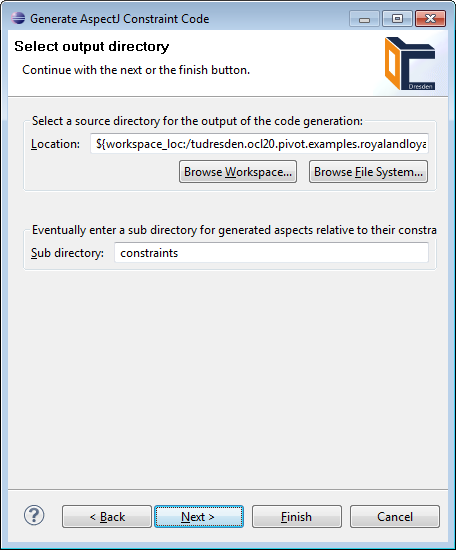
\includegraphics[width=1.0\linewidth]{figures/codegen/codegen03}
	\caption{The third step: Selecting a target directory for the generated code.}
	\label{pic:codegen:codegen03}
\end{figure}


\newpage
\subsection{Specifying General Settings}
	
On the following page of the wizard we can specify general settings for the code generation (see Figure \ref{pic:codegen:codegen04}).

\begin{figure}[!b]
	\centering
	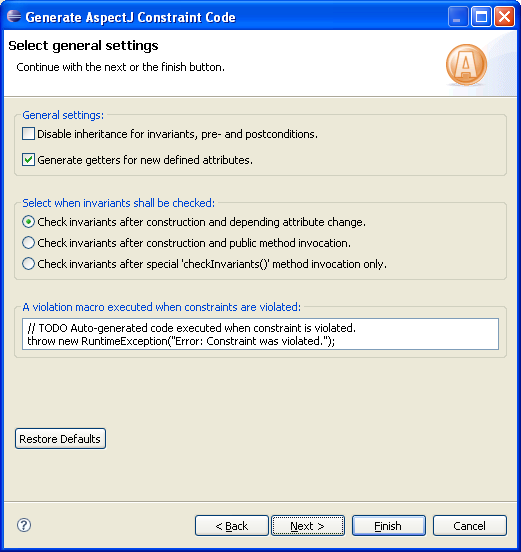
\includegraphics[width=1.0\linewidth]{figures/codegen/codegen04}
	\caption{The fourth step: General settings for the code generation.}
	\label{pic:codegen:codegen04}
\end{figure}

We can disable the inheritance of constraints (which would not be useful in our example because we want to enforce the constraint for \model{Persons}, but for \model{Students} and \model{Professors} as well). We can also enable that the code generator will generate getter methods for newly defined attributes of \model{def} constraints. More interesting is the possibility to select one of three provided strategies, when invariants shall be checked during runtime:

\begin{enumerate}
	\item Invariants can be checked after construction of an object and after any change of an attribute or association which is in scope of the invariant condition (\keyword{Strong Verification}).
	\item Invariants can be checked after construction of an object and before or after the execution of any public method of the constrained class (\keyword{Weak Verification}).
	\item And finally, invariants can only be checked if the user calls a special method at runtime (\keyword{Transactional Verification}).
\end{enumerate}

These three scenarios can be useful for users in different situations. If a user wants to verify strongly, that his constraints are verified after any change of any dependent attribute he should use \keyword{Strong Verification}. If he wants to use attributes to temporary store values and constraints shall only be verified if any external class instance wants to access values of the constrained class, he should use \keyword{Weak Verification}. If the user wants to work with databases or other remote communication and the state of his constraint classes should be only valid before data transmission, he should use the scenario \keyword{Transactional Verification}.

Finally, we can specify a \keyword{Violation Macro} which specifies the code, which will be executed when a constraint is violated during runtime. By default, the violation macro throws a run-time exception. We also want to have a run-time exception thrown when our constraint is violated. Thus, we do not change the violation macro and continue with the \eclipse{Next} button.


\newpage
\subsection{Constraint-Specific Settings}

The last page of the code generation wizard provides the possibility to configure some of the code generation settings constraint-specific by selecting a constraint and adapting it's settings (see Figure \ref{pic:codegen:codegen05}). We don't want to adapt the settings, thus we can finish the wizard and start the code generation by clicking the \eclipse{Finish} button.

\begin{figure}[!b]
	\centering
	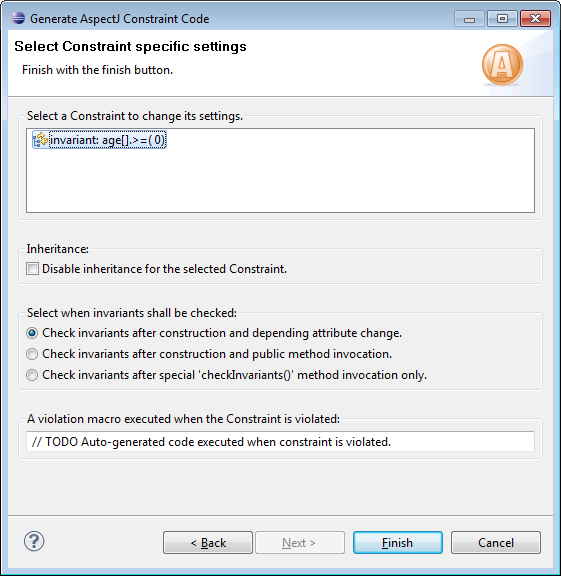
\includegraphics[width=1.0\linewidth]{figures/codegen/codegen05}
	\caption{The fifth step: Constraint-specific settings for the code generation.}
	\label{pic:codegen:codegen05}
\end{figure}



\newpage
\section{The Generated Code}

After finishing the wizard, the code for the selected constraint will be generated. To see the result, we have to refresh our project in the workspace. We select the project \model{tudresden.ocl20.pivot.\linebreak[0]examples.simple.constraint} in the \eclipse{Package Explorer} open the context menu by a right mouse click and select the menu item \eclipse{Refresh}. Afterwards, our project contains a new generated AspectJ file called \model{tudresden.ocl20.pivot.examples.simple.constraints.InvAspect\-01.aj} (see Figure \ref{pic:codegen:packageExplorer}). Now we can rerun our JUnit test case. The test case finishes successfully because the expected run-time exception is thrown (see Figure \ref{pic:codegen:junit02}).	

\begin{figure}[!b]
	\centering
	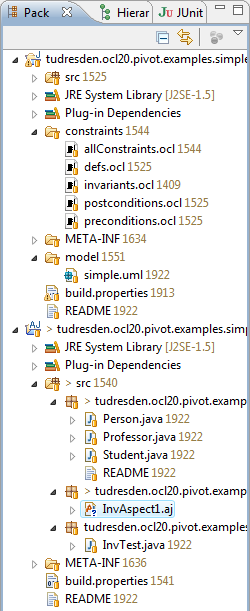
\includegraphics[width=0.5\linewidth]{figures/codegen/packageExplorer}
	\caption{The package explorer containing the new generated aspect file.}
	\label{pic:codegen:packageExplorer}
\end{figure}


\begin{figure}[!htbp]
	\centering
	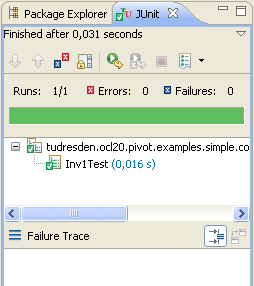
\includegraphics[width=0.5\linewidth]{figures/codegen/junit02}
	\caption{The successfully finished jUnit test case.}
	\label{pic:codegen:junit02}
\end{figure}


	
\section{Summary}
  
This Chapter described how to generate AspectJ code using the \keyword{OCL22Java} code generator of \acl{DOT4Eclipse}. A more detailed documentation of the OCL22Java code generator can be found in the Minor Thesis (Gro�er Beleg) of Claas Wilke \cite{GB:Wilke}.
\chapter{SQL Code Generation}
\label{chapter:ocl2sql}

\begin{flushright}
\textit{Chapter written by Bj�rn Freitag}
\end{flushright}

This chapter describes how the SQL Code Generator \keyword{OCL2SQL} provided 
with Dresden OCL can be used. A general introduction into Dresden OCL can 
be found in Chapter~\ref{chapter:introduction}. 

Actual the SQL Code Generator is able to generate the following SQL dialects:
\begin{itemize}
  \item Standard SQL
  \item PostgreSQL
  \item Oracle SQL
  \item MySQL
\end{itemize}



\section{Code Generator Preparation}
This chapter uses the \keyword{University Example} which is provided with 
Dresden OCL. The example is show in Figure~\ref{pic:example:university01}. To
import the university example into our Eclipse workspace we simply have to use
the wizard \emph{File -> New -> Other\ldots -> Dresden OCL Examples ->
University Example (UML)}. Afterwards, the project 
\model{tudresden.ocl20.pivot.\linebreak[0]examp\-les.\linebreak[0]university})
should exist within the workspace.

The project 
provides a model file which contains the university class diagram (the model file is located at 
\model{model/university.uml}) and the constraint file we want to generate code for 
(located at
\model{con\-straints/\linebreak[0]uni\-ver\-si\-ty\linebreak[0].ocl}). One
invariant is shown in Listing~\ref{lst:codegen:universityInvariant}. It is contained in the
constraint file we want to generate code for. The invariant declares, that the
\model{grade} of any \model{Person}'s superviser must be greater thant its own
\model{grade}.

\begin{figure}[!t]
	\centering
	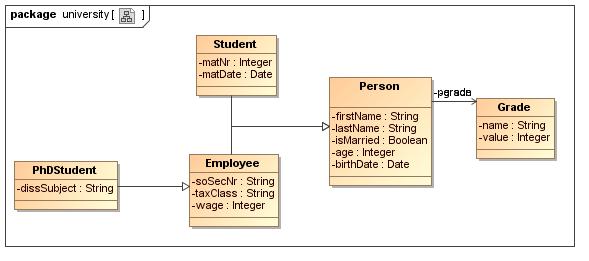
\includegraphics[width=0.85\linewidth]{figures/examples/university01}
	\caption{the UML diagram of the university example.}
	\label{pic:example:university01}
\end{figure}

\begin{figure}[!htbp]
  \lstset{
    language=OCL
  }
  \begin{lstlisting}[caption={a simple invariant.}, captionpos=b, label=lst:codegen:universityInvariant]
context Person
inv tudOclInv1: self.supervisor.grade.value > self.grade.value
  \end{lstlisting}
  
\end{figure}



\section{Code Generation}
To prepare the code generation we have to import the model 
\model{model/university.uml} into the \eclipse{Model Browser}. We use the model
import wizard of Dresden OCL to import the model. This procedure is explained in
Chapter~\ref{chapter:introduction}. Afterwards, we have to open the constraint
file \model{con\-straints/\linebreak[0]university.ocl}. After the 
importation, the \eclipse{Model Browser} should look like illustrated in 
Figure~\ref{pic:codegen:modelBrowserSQL}. Now we can start the code generation.
By selecting the item \eclipse{Generate SQL Code} of the menu \eclipse{Dresden
OCL} the sql code generation can be started.

\begin{figure}[!b]
	\centering
	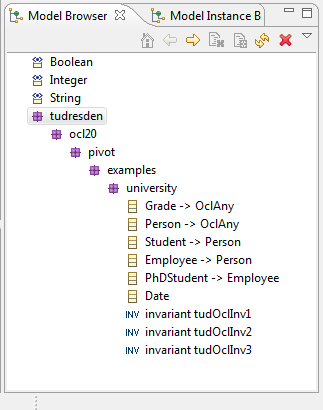
\includegraphics[width=0.45\linewidth]{figures/codegen/modelBrowserSQL}
	\caption{The Model Browser containing the University Model and its Constraints.}
	\label{pic:codegen:modelBrowserSQL}
\end{figure}


\subsection{Selecting a Model}
A wizard opens and we have to select a model for code generation (cf. 
Fig.~\ref{pic:codegen:codegen01SQL}). We select the \model{university.uml} model
and click the \eclipse{Next} button.

\begin{figure}[!p]
	\centering
	\includegraphics[width=1.0\linewidth]{figures/codegen/codegen01SQL}
	\caption{The first Step: Selecting a Model for Code Generation.}
	\label{pic:codegen:codegen01SQL}

	\vspace{2.0em}
	
	\centering
	\includegraphics[width=1.0\linewidth]{figures/codegen/codegen02SQL}
	\caption{The second Step: Selecting Constraints for Code Generation.}
	\label{pic:codegen:codegen02SQL}
\end{figure}


\subsection{Selecting Constraints}
As a second step we have to select the constraints we want to
generate code for. We only select the constraints \model{inv: oclInv1} and
\model{inv: oclInv2}. After selecting the constraints we click on the
\eclipse{Next} button (cf. Fig.~\ref{pic:codegen:codegen02SQL}).

\begin{figure}[!p]
	\centering
	\includegraphics[width=1.0\linewidth]{figures/codegen/codegen03SQL}
	\caption{The third Step: Selecting a target directory for the Generated Code.}
	\label{pic:codegen:codegen03SQL}

	\vspace{2.0em}
	
	\centering
	\includegraphics[width=1.0\linewidth]{figures/codegen/codegen04SQL}
	\caption{The fourth Step: General Settings for the Code Generation.}
	\label{pic:codegen:codegen04SQL}
\end{figure}


\subsection{Selecting a target directory}
Now, we have to choice the directory where the generated code will be stored.
We select the folder \model{sql} in this project (which is 
\model{tudresden.\linebreak[0]ocl20.pivot.examples.university/\linebreak[0]sql})
(cf. Fig.~\ref{pic:codegen:codegen03SQL}). We can click the \eclipse{Next}
button.

On the following page of the wizard we can specify general settings for the code
generation (cf. Fig.~\ref{pic:codegen:codegen04SQL}). We can choice a SQL
dialect for the generated code. The modus of SQL generation decides how
inheritance relationships are described in the SQL schema. In the typed
modus all subclass properties will be written to the table of the super class.
Any class has its own table with the own properties in the vertical modus. If
you wish only to generate the code for invariant you must choice \emph{Only
Integrity View} otherwiese the table schema will be generated as well. The other
parameter will set the prefix for the different parts of the SQL schema. We can
finish the settings and start the code generation with the \eclipse{Finish} button.



\section{The Generated Code}
After finishing the wizard, the code for the selected constraints will be 
generated. To investigate the results it can be necessary to refresh the
project (F5). Our project contains two new SQL files in the folder \texttt{sql}
(cf. Fig.~\ref{pic:codegen:projectExplorerSQL}). The file 
\texttt{2010-09-29-09-34\_schema.sql} has the table and view schema of the
model. Every class of the model has its own view. Over this view the
data(object) of the class can be accesssed. The other file
\texttt{2010-09-29-09-34\_view.sql} has the views for the invariants (cf.
Fig.~\ref{pic:codegen:generateSQL}). The views contain all objects that
violtate the specific invariant (cf. Listing~\ref{lst:codegen:sqlInvariant}).

\begin{figure}[!p]
	\centering
	\includegraphics[width=0.45\linewidth]{figures/codegen/projectExplorerSQL}
	\caption{The Package Explorer containing the new SQL code files.}
	\label{pic:codegen:projectExplorerSQL}

	\vspace{2.0em}
	
	\centering
	\includegraphics[width=0.45\linewidth]{figures/codegen/generateSQL}
	\caption{The Package Explorer containing the new SQL code files.}
	\label{pic:codegen:generateSQL}

	\vspace{2.0em}
	
 \lstset{
    language=SQL
 }
 \begin{lstlisting}[caption={SQL Code for invariant oclInv1.}, captionpos=b,
  label=lst:codegen:sqlInvariant] -- Context: Person
-- Expression: inv tudOclInv1: self.supervisor.grade.value > self.grade.value
CREATE OR REPLACE VIEW tudOclInv1 AS
(SELECT * FROM OV_Person AS SELF
WHERE NOT (((SELECT value FROM OV_Grade
 WHERE PK_Grade IN (SELECT FK_grade FROM OV_Person
 WHERE PK_Person IN (SELECT FK_supervisor FROM OV_Person WHERE PK_Person = SELF.PK_Person))) > (SELECT value FROM OV_Grade
 WHERE PK_Grade IN (SELECT FK_grade FROM OV_Person WHERE PK_Person = SELF.PK_Person)))));
  \end{lstlisting}
\end{figure}

\section{Summary}
  
How to generate SQL code using the 
\keyword{OCL2SQL} code generator of Dresden OCL was described in this chapter.
Besides the use of \keyword{OCL2SQL} via Dresden OCL's GUI, you can also invoke
OCL2SQL via Dresden OCL's \acs{API}. The easiest way to connect to Dresden OCL
is via its \emph{Facade} providing interfaces for all services of Dresden OCL. 
How to use Dresden OCL's facade is documented in Chapter~\ref{chapter:integration}.

\chapter{Dresden OCL Metrics}
\label{chapter:metrics}

\begin{flushright}
\textit{Chapter written by Claas Wilke}
\end{flushright}

This chapter describes how the Dresden OCL Metrics tool provided with Dresden
OCL can be used. A general introduction into Dresden OCL can be found in
Chapter~\ref{chapter:introduction}.
This chapter uses the \keyword{Simple Example} which is provided with 
Dresden OCL and has been introduced in Section~\ref{intro:simpleExample}. 



\section{Using Dresden OCL Metrics}

The Dresden OCL Metrics tool is a simple tool that allows to compute some
statistics for a selected or a set of selected OCL constraints.

In summary, the following metrics can be computed:

\begin{itemize}
  \item The number of constraints selected,
  \item The number of constraints by kind (Body, Definition, Derived,
  Init, Invariant, Postcondition, Precondition),
  \item The number of expressions used within the selected constraints
  (including minimum, maximum, average, and median number of expressions per
  constraint),
  \item The depth of the expressions within the selected constraints (minimum,
  maximum, average, and median),
  \item The number of if-expressions used within the selected constraints,
  \item The number of let-expressions used within the selected constraints,
  \item The number and kinds of literals used within the selected constraints,
  \item The number and kinds of iterators used within the selected constraints,
  \item The number and names of operations called within the selected
  constraints,
  \item The number and names of properties called within the selected
  constraints.
\end{itemize}

Dresden OCL Metrics consists of a single view that should be visible at the
center bottom of the Dresden OCL perspective (cf.
Fig.~\ref{pic:metrics:metrics01}). If not, the view can be opened by the menu
option \emph{Dresden OCL -> Open OCL Metrics}.

\begin{figure}[!t]
	\centering
	\includegraphics[width=1.0\textwidth]{figures/metrics/metrics01.png}
	\label{pic:metrics:metrics01}
	\caption{The Dresden OCL perspective showing the Dresden OCL Metrics view at
	the center bottom.}
\end{figure}

Any time, you select a set of constraints or a model element containing a set of
constraints within the \emph{Model Browser}, the results will be automatically
displayed within the \emph{Dresden OCL Metrics View} (cf.
Fig~\ref{pic:metrics:metrics01}).

	
\section{Summary}
  
This chapter described how to use the Dresden OCL Metrics. Feel free to explore
the metrics using your own example. If you have ideas for further metrics,
please do not hesitate to let us know. Maybe we will implement your metrics
within a following version of Dresden OCL \ldots


\part{Tool Development using Dresden OCL}

\chapter{The Architecture of Dresden OCL}
\label{chapter:architecture}

\begin{flushright}
\textit{Chapter written by Claas Wilke}
\end{flushright}

This chapter introduces into the highly generic architecture of Dresden OCL.
Before the architecture is explained, some theoretical background is shortly 
presented. Further details of Dresden OCL's architecture can be found
in~\cite{braeuerEA:OCL2007} and~\cite{wilkeEA:MODELS2010}.



\section{The Generic Three Layer Metadata Architecture}
\label{architecture:genericLayers}

The \acl{OCL} is a language that is always based on another modeling language 
(usually the \acs{UML}). Without another language used for modeling, it does 
not make any sense to define constraints because \acs{OCL} is used for
constraint specification but not for modeling itself. Thus, besides \acs{OCL}, 
a modeling language is required to define a model on that \acs{OCL} constraints 
can be specified.

Each modeling language is defined in another language, its 
\keyword{Meta-Modeling Language}. For example, the \acl{UML}'s meta-model is 
defined using the \keyword{\acf{MOF}}~\cite{spec:MOF2.0}, the standardized
meta-meta model of the \acs{OMG}. The \acs{MOF} is used to describe the 
\acs{UML} meta-model that can be used to model \acs{UML} models. Generally 
spoken, each model requires a meta-model that is used to describe the model. 
The model can be instantiated by model instances (for example a \acs{UML} class 
diagram can be instantiated by a \acs{UML} object diagram). The model can be 
enriched with \acs{OCL} constraints that are defined on the model (using an 
\acs{OCL} meta-model / abstract syntax) and can then be verified for instances
of the model afterwards.

The \acs{OMG} introduced the \keyword{\acs{MOF} Four Layered Metadata
Architecture} \cite{spec:MOF2.0}\cite[p. 16ff]{spec:UML2-2Inf} that is used to 
arrange and structure the meta-model, the model, and the model's instances into 
a layered hierarchy (see Figure~\ref{pic:architecture:mofLayers}). Generally, 
four layers can be identified, the \keyword{Meta-Meta-Model Layer (M3)}, the
\keyword{Meta-Model Layer (M2)}, the \keyword{Model Layer (M1)}, and the 
\keyword{Model Instance Layer (M0)}. The latest version of \acs{MOF} allows to
define as much layers as required for a certain use
case~\cite[p.~8f]{spec:MOF2.0}. 

\begin{figure}[!t]
	\centering
	\includegraphics[width=.4\linewidth]{figures/architecture/mofLayers}
	\caption{The MOF Four Layer Metadata Architecture.}
	\label{pic:architecture:mofLayers}
\end{figure}

\begin{sidewaysfigure}[!p]
	\centering
	\includegraphics[width=1.0\linewidth]{figures/architecture/genericLayers}
	\caption{The Generic Three Layer Metadata Architecture.}
	\label{pic:architecture:genericLayers}
\end{sidewaysfigure}

\acs{OCL} constraints can be defined on both, meta-models and models to verify 
models or model instances, respectively. E.g., one may use \acs{OCL} to define 
rules on a meta-model that must be ensured for every model modeled with the 
meta-model. But, one may use \acs{OCL} to define rules on a model (that must be
verified for the model's instances) as well. Thus, the four layer metadata 
architecture can be generalized to a \keyword{Generic Three Layer Metadata 
Architecture}~\cite{demuth:RGWS09} in the scope of an \acs{OCL} definition (see 
Figure~\ref{pic:architecture:genericLayers}). 

On the \keyword{Mn+1 Layer} lies 
the meta-model that is used to define the model that shall be constrained. The
\acs{OCL} abstract syntax extends the meta-model to allow contexts of \acs{OCL}
constraints refering to elements of the model.

On the \keyword{Mn Layer} lies the model that is an instance of the meta-model
and can be enriched by the specification of \acs{OCL} constraints. 

Finally, on the \keyword{Mn-1 Layer} lies the model instance on that the 
\acs{OCL} constraints shall be verified. Please note that in the context of 
such a generic layer architecture, a model instance can be both a model (like a
\acs{EMF} Ecore model in Figure~\ref{pic:architecture:genericLayers}~(c))) or a
set of objects (like Java run-time objects in
Figure~\ref{pic:architecture:genericLayers}~(b)). To provide a relationship
between the model instance's elements and the model's elements a mapping is
required between both. Thus, the model instance requires a description of a
model realisation that allows to reflect on the instance's elements (e.g., for
Java run-time objects such a realisation can be considered as a set of Java
classes. Each \code{java.lang.Object} allows to reflect on its
\code{java.lang.Class}. This \code{Class} can then be mapped to the
corresponding model element in the model by comparing the \code{Class}es name
with the names of \code{Type}s existing in the model).



\section{Dresden OCL's Package Architecture}

The package architecture of Dresden OCL is shown in
Figure~\ref{pic:architecture:modules}. The architecture can be separated into
five layers: 

\begin{enumerate}
  \item The \keyword{API Layer},
  \item the \keyword{Tools Layer},
  \item the \keyword{Registry Layer},
  \item the \keyword{\acs{OCL} Layer},
  \item and the \keyword{Variability Layer}.
\end{enumerate}

\begin{figure}[!b]
	\centering
	\includegraphics[width=1.0\linewidth]{figures/architecture/modules}
	\caption{The package architecture of Dresden OCL.}
	\label{pic:architecture:modules}
\end{figure}

The API layer provides the Facade of Dresden OCL that can be used by other
plug-ins to access the \acs{OCL} tools of Dresden OCL. The Facade of Dresden OCL
is introduced in Chapter~\ref{chapter:integration}.

The Tools Layer contains the Tools provided by Dresden OCL. These are: The
\acs{OCL} Parser/Editor introduced in Section~\ref{intro:oclEditor}, the
\acs{OCL} Interpreter introduced in Chapter~\ref{chapter:interpretation} and the
\acs{OCL}22Java Code Generator introduced in
Chapter~\ref{chapter:codeGeneration}. Finally, the \keyword{Model Browser} can
be used to store imported models, and model instances. The backend of the Model
Browser is the \keyword{Model Bus} that manages all meta-models and model
instance types currently provided by Dresden OCL. The model bus is located at the
Registry Layer.
\todocw{Add OCL22SQL here when available.}

The \acs{OCL} layer contains the \acs{OCL} syntax and semantics used by the
tools of Dresden OCL. The \acs{OCL} syntax and semantics are separated into
three different packages. \keyword{Essential OCL} contains the abstract syntax
(or meta-model) of \acs{OCL} that is used by Dresden OCL and its tools. The
\keyword{OCL Standard Library Model} provides a modeled description of all
operations that are provided by the \acs{OCL} Standard Library (as defined in
\cite[Ch.~11]{spec:OCL2-2}). Finally the \keyword{OCL Standard Library
Semantics} provides an implementation of all these operations that are used by
the \acs{OCL} Interpreter of Dresden OCL for \acs{OCL} interpretation.

The last layer is the Variability Layer. The Variability layer contains the
\keyword{Pivot Model} and the \keyword{Model Instance Types} that are used to
connect Dresden OCL with various meta-models or types of model instances,
respectively. The Pivot Model is described more detailed in
Section~\ref{architecture:metaModelAdaptation}, the Model Instance Types are
explained in Section~\ref{architecture:modelInstanceAdaptation}. Further details
on both the Pivot Model and the Model Instance Types can be found 
in~\cite{braeuerEA:OCL2007} and~\cite{wilkeEA:MODELS2010}.

Dresden OCL has been developed as a set of Eclipse/\acs{OSGi} plug-ins. All
packages represent different Eclipse plug-ins. Additionally, \acl{DOT4Eclipse}
contains some plug-ins to provide \acs{GUI} elements such as wizards and 
examples to run \acl{DOT4Eclipse} with some simple models and \acs{OCL} 
expressions. An overview over all plug-ins provided with \acl{DOT4Eclipse} can
be found in Table~\ref{tab:plugins} in the appendix of this manual.



\section{Dresden OCL and the Generic Three La\-yer Me\-ta\-da\-ta Architecture}
\label{theory:DOTLayers}

\begin{sidewaysfigure}
	\centering
	\includegraphics[width=1.0\linewidth]{figures/architecture/modeladaptation}
	\caption{The architecture of Dresden OCL with respect to the Generic Three Layer
	Metadata Architecture.}
	\label{pic:architecture:genericArchitecture}
\end{sidewaysfigure}

Figure~\ref{pic:architecture:genericArchitecture} shows the architecture of 
Dresden OCL with respect to the Generic Three Layer Metadata Architecture
(introduced in Section~\ref{architecture:genericLayers}). At the first sight, 
the architecture seems to be very complex. But do not be afraid! The 
architecture will now be explained step by step.


\subsection{The Adaptation of Meta-Models, Models and Model Instances}

As you can see, the left part of 
Figure~\ref{pic:architecture:genericArchitecture} shows the Generic Three Layer
Metadata Architecture. Meta-models, models and model instances are adapted and 
loaded into Dresden OCL. It could be argued that such an adaptation is expensive
and costly, but the opposite is the truth. The architecture of Dresden OCL allows
its users to adapt the toolkit to every meta-model and model instance type they 
want to. After the adaptation of a new meta-model or model-instance type, they
can reuse the complete set of tools provided by Dresden OCL! Thus,
to adapt the \acs{OCL} Interpreter to a new type of model instance, only one 
adaptation is required. The rest comes for free!


\subsection{How Meta-Models and Models are Adapted}
\label{architecture:metaModelAdaptation}

As already said, the core feature of Dresden OCL is the \keyword{Pivot Model}
(a.k.a. \keyword{Model Types}). The pivot model is a meta-model that abstracts
from all other meta-models. It contains interfaces to define the structural 
parts of a model such as
\code{Types}, \code{Namespaces}, \code{Operations} and \code{Properties}. 
Furthermore, these interfaces provide methods to reason on them (e.g., the 
interface \code{Namespace} provides a method \code{getNestedNamespaces()} to 
retrieve all contained \code{Namespaces}).

Every meta-model users want to work with can be adapted to the pivot model. The
\keyword{Adapted Meta-Model} must implement the interfaces of the pivot model 
and must adapt them to its meta-model elements. E.g., adapting the \acs{UML}2 
meta-model, the interface \code{Type} from the pivot model must be adapted to 
the meta-model element \code{UML2Class}. Besides the adaptation of the pivot 
model, each meta-model must provide a \code{ModelProvider} that provides 
methods to load model resources of the adapted meta-model and adapts them to 
its pivot model implementation. The result is an \keyword{Adapted Model},
Dresden OCL can work with. Further details about the adaptation of meta-models to
the pivot model can be found in Chapter~\ref{chapter:pivotModelAdaptation}.


\subsection{How Model Instances are Adapted}
\label{architecture:modelInstanceAdaptation}

If the \acs{OCL} Interpreter shall be used to interpret instances of amn opened 
model, a second adaptation is required, an adaptation to the \keyword{Model 
Instance Type Model}. The model instance type model can be considered as similar
to the pivot model, but the purpose is different. If \acs{OCL} constraints shall
be interpreted on run-time objects or values, operations and properties of these
run-time values must be accessible. E.g., if a constraint like \code{context 
Person inv: age >= 0} shall be interpreted, the property \code{age} of a
run-time object of the class \code{Person} must be accessed. The \acs{OCL} 
interpreter does not accesses this property directly, but delegates the request 
to a \keyword{Model Instance Element} adaptation to let the model instance type
become exchangeable\footnote{To be honest, the interpreter does not access the
model instance element directly but uses the \acs{OCL} standard library
semantics instead which delegate the request to the model instance element. But
this is a technical detail and not important in this context.}. Thus,
Dresden OCL contains a second model the \keyword{Model Instance Types}
that can be considered as an abstraction of all model instance types. The model 
instance types define a set of interfaces to describe the elements of a model 
instance (e.g., \code{IModelInstancePrimitiveType} and 
\code{IModelInstanceObject}). These interfaces provide operations to reflect on 
the model instance elements (e.g., the operation
\code{IModelInstanceType.invokeOperation()} or the operation 
\code{IModelInstanceElement.isTypeOf()}). The reflection mechanism can be 
considered as similar to the mechanism provided by Java in the package 
\code{java.lang.reflect}.

Each model instance type users want to work with must be adapted to the model 
instance types. Besides an adaptation of the interfaces, also a 
\code{ModelInstanceProvider} must be implemented that is responsible to adapt 
model instance objects to the implemented interfaces. Due to the fact of this 
second adaptation, Dresden OCL is able to use the same \acs{OCL} Interpreter for
different types of model instances! More details about the adaptation of model 
instances to Dresden OCL are available in 
Chapter~\ref{chapter:modelInstanceTypeAdaptation}.


\subsection{Coupling between Models and their Instances}

As mentioned above, different types of models can be connected with different 
types of instances. E.g., a \acs{UML} class diagram could be implemented by a 
set of Java Classes (and their objects) or by an \acs{XML} document. To 
maintain this loose coupling, meta-models and model implementation types do not 
know each other. If a model instance is imported into Dresden OCL, a model (and
thus also a meta-model) has to be selected, to that the instance belongs to. The
objects of the instance are matched to the types of the selected model by the 
name of their types. E.g., a Java instance's \code{Object}s are matched by
associating their \code{Class}es' names to the names of the types of the
selected model.



\section{Summary}

This Chapter introduced into the architecture and package structure of
Dresden OCL. The \keyword{Pivot Model} and the \keyword{Model Instance Types} 
have been explained shortly. Also the relationships between the pivot model, 
\keyword{Essential \acs{OCL}} and the \keyword{\acs{OCL} Standard Library} have
been presented. One may argue that the architecture seems to be complex and 
complicate. Nevertheless, it should be remembered that Dresden OCL was 
designed as generic as possible. Thus, Dresden OCL can be adapted to various
different kinds of meta-models and model instances without changing the
\acs{OCL} Parser nor the \acs{OCL} Interpreter! The currently existing
adaptations to meta-models and model instances are documented in
Section~\ref{sect:info:models} and Section~\ref{sect:info:modelinstances},
respectively.

\chapter{How to integrate Dresden OCL2 for Eclipse}
\label{chapter:integration}

\begin{flushright}
\textit{Chapter written by Claas Wilke}
\end{flushright}

In Chapter \ref{chapter:architecture} the architecture of \acl{DOT4Eclipse} has shortly been explained. This chapter will explain, how \acl{DOT4Eclipse} can be integrated into other tools, toolkits or projects.



\section{The Integration Facade of Dresden OCL2 for Eclipse}

Since the release 2.1.0, \acl{DOT4Eclipse} contains an \keyword{Integration Facade}, that combines all required interfaces of \acl{DOT4Eclipse} in one interface, also called a \keyword{Facade} \cite{gamma:dp}. The facade contains self-explanatory static methods that provide access to the repository (modelbus) and all tools of \acl{DOT4Eclipse}. A documentation of the complete facade's interface would be too large for this documentation. Thus, please investigate the facade directly in the code. The facade called \code{Ocl2ForEclipseFacade} is located in the plug-in \code{tudresden.ocl20.pivot.facade}. Please be aware of the fact that if you use the facade, you will result in dependencies to all major parts of \acl{DOT4Eclipse}. Thus, if you want to use one of the tools only (e.g, the \acs{OCL}2 Parser) you could access these tools directly as explained below.



\section{How to access Meta-Models, Models and Instances}

The central component of \acl{DOT4Eclipse} is the \keyword{Model-Bus} which is implemented by the Eclipse plug-in \code{tudresden.ocl20.pivot.modelbus}. The main class of this plug-in (\code{tudresden.\linebreak[0]ocl20.pivot.modelbus.ModelBusPlugin}) provides methos, to access meta-models, models and model instances and to import new resources of these kinds into the toolkit (see Figure \ref{pic:integration:modelBusPlugin}).

The class provides four different static methods to access different registries, the \code{Meta\-model\-Re\-gis\-try}, the \code{ModelRegistry}, the \code{ModelInstanceTypeRegistry} and the \code{ModelInstanceRegistry}.

\begin{figure}[!b]
	\centering
	\includegraphics[width=.8\linewidth]{figures/integration/modelBusPlugin}
	\caption{The main class of the Model-Bus plug-in.}
	\label{pic:integration:modelBusPlugin}
\end{figure}


\subsection{The Meta-Model Registry}

The Meta-Model Registry provides methods to add and get meta-models to and from \acl{DOT4Eclipse}. Normally, the method \code{addMetamodel(IMetamodel)} is not required because by starting Eclipse, all meta-models register themselves via their extension point in the registry. To get a meta-model from the toolkit, the methods \code{getMetamodels()} and \code{getMetamodel(id: String)} can be used. The method \code{getMetamodels()} returns all meta-models that are currently registered in the registry. The method \code{getMetamodel(id: String)} can be used to get a meta-model by its ID (Normally, the ID of a meta-model is equal to the name of its plug-in. E.g., the \acs{UML}2 meta-model has the ID \code{tudresden.ocl20.pivot.metamodels.uml2}).

\begin{figure}[!b]
	\centering
	\includegraphics[width=.55\linewidth]{figures/integration/metaModelRegistry}
	\caption{The Meta-Model Registry.}
	\label{pic:integration:metaModelRegistry}
\end{figure}


\subsection{How to load a Model}

First, to load a model into \acl{DOT4Eclipse}, the meta-model the model is an instance of has to be selected . E.g., for an \acs{UML}2 class diagram the \acs{UML}2 meta-model should be selected (see Listing \ref{lst:integration:loadModel}). Each meta-model has its own \code{IModelProvider} that can be accessed by using the method \code{IMetamodel.getModelProvider()}. The \code{IModelProvider} provides three methods to load a model. A model can be loaded by using the method \code{getModel(..)} with

\begin{enumerate}
	\item A \code{File} object representing the model as argument,
	\item a \code{String} representing the path of the file there the model is located,
	\item or a \code{URL} leading to the file there the model is located.
\end{enumerate}

\lstset{
  language=Java
}
\begin{lstlisting}[caption={How to load a model.}, captionpos=b, label=lst:integration:loadModel, float]
IMetamodel metaModel;
IModel model;

metaModel = ModelBusPlugin.getMetamodelRegistry()
              .getMetamodel("tudresden.ocl20.pivot.metamodels.uml2");
model = metaModel.getModelProvider().getModel(modelURL);
\end{lstlisting}

\begin{figure}[!b]
	\centering
	\includegraphics[width=.55\linewidth]{figures/integration/modelRegistry}
	\caption{The Model Registry.}
	\label{pic:integration:modelRegistry}
\end{figure}

After loading the model, the model can be added to the \code{ModelRegistry}, that manages all models currently loaded into \acl{DOT4Eclipse} (see Figure \ref{pic:integration:modelRegistry}). The \code{ModelRegistry} can also be used to set an active model which represents the \code{IModel} that is currently selected in the \keyword{Model Browser} of \acl{DOT4Eclipse}.


\subsection{The Model Instance Type Registry}

Similar to the Meta-Model Registry, the Model Instance Type Registry provides methods to add and get model instance types to and from \acl{DOT4Eclipse}. Normally, the method \code{addModelInstanceType(IModelInstanceType)} is not required because by starting Eclipse, all model instance types register themselves via their extension point in the registry. To get a model instance type from the toolkit, the methods \code{getModelInstanceTypes()} and \code{getModelInstance\-Type\linebreak[0](id: String)} can be used. The method \code{getModelInstanceTypes()} returns all model instance types that are currently registered in the registry. The method \code{getModelInstanceType(id: String)} can be used to get a model instance types by its ID (Normally, the ID of a model instance type is equal to the name of its plug-in. E.g., the Java model instance type has the ID \code{tudresden.ocl20.pivot.modelinstancetype.java}).

\begin{figure}[!b]
	\centering
	\includegraphics[width=.7\linewidth]{figures/integration/modelInstanceTypeRegistry}
	\caption{The Model Instance Type Registry.}
	\label{pic:integration:modelInstanceTypeRegistry}
\end{figure}


\subsection{How to load a Model Instance}

First, to load a model instance into \acl{DOT4Eclipse}, the model instance type must be selected the instance is an instance of. E.g., for a set of Java objects the Java model instance type should be selected (see Listing \ref{lst:integration:loadModelInstance}). Each model instance type has its own \code{IModelInstanceProvider} that can be accessed by using the method \code{IModelInstanceType.get\-Mo\-del\-Instance\-Provider}. The \code{IModelInstanceProvider} provides three methods to load a model instance. A model instance can be loaded by using the method \code{getModelInstance(..)} with

\begin{enumerate}
	\item A \code{File} object representing the model instance as argument,
	\item a \code{String} representing the path of the file there the model instance is located,
	\item or a \code{URL} leading to the file there the model instance is located.
\end{enumerate}

Additionally, each of these methods requires the \code{IModel} as a second argument, the model instance is an instance of. Thus, the model must be loaded before the model instance can be loaded.

\lstset{
  language=Java
}
\begin{lstlisting}[caption={How to load a model instance.}, captionpos=b, label=lst:integration:loadModelInstance, float]
IModelInstanceType miType;
IModelInstance modelInstance;

miType = ModelBusPlugin.getModelInstanceTypeRegistry()
           .getModelInstanceType(
             "tudresden.ocl20.pivot.modelinstancetype.java");
modelInstance = miType.getModelInstanceProvider()
                  .getModelInstance(modelInstanceUrl, model);
\end{lstlisting}

\begin{figure}[!b]
	\centering
	\includegraphics[width=.75\linewidth]{figures/integration/modelInstanceRegistry}
	\caption{The Model Instance Registry.}
	\label{pic:integration:modelInstanceRegistry}
\end{figure}

After loading the model instance, the model instance can be added to the \code{Model\-Instance\-Re\-gis\-try}, that manages all model instances currently loaded into \acl{DOT4Eclipse} (see Figure \ref{pic:integration:modelInstanceRegistry}). The \code{ModelInstanceRegistry} can also be used to set an active model instance that represents the \code{IModelInstance} that is currently selected in the \keyword{Model Instance Browser} of \acl{DOT4Eclipse}.



\section{How to access the OCL2 Parser}

The \acs{OCL}2 Parser of \acl{DOT4Eclipse} is located in the plug-in \code{tudresden.ocl20.pivot.\linebreak[0]ocl\-2\-Parser}. The parser provides a very simple interface and can be used as shown in Listing \ref{lst:integration:parserConstraints}. First a \code{Reader} used to read all constraints that shall be parsed has to be created, and an \code{IModel} for that the constraints shall be parsed has to be loaded. Afterwards, the method \code{OCL2Parser.doParse()} can be invoke on the singleton instance of the parser to parse the constraints.

\begin{figure}[!b]
\begin{lstlisting}[caption={How to parse constraints.}, captionpos=b, label=lst:integration:parserConstraints]
FileReader oclFileReader;
OCL2Parser parser;
List<Constraint> parsedConstraints;

oclFileReader = new FileReader(oclFile);
parsedConstraints = Ocl2Parser.INSTANCE.doParse(model, reader);
\end{lstlisting}
\end{figure}



\section{How to access the OCL2 Interpreter}

To use the \acs{OCL}2 Interpreter, a model and a model instance must be loaded into the toolkit before. Additionally, at least one constraint must be parsed that shall be interpreted for the objects contained in the model instance. The interpreter is located in the plug-in \code{tudresden.ocl20.pi\-vot.\linebreak[0]in\-ter\-pre\-ter}. It has a more complex interface than the other tools and contains many different operations to interpret different kinds of constraints.

\begin{figure}[!b]
\begin{lstlisting}[caption={How to interpret constraints.}, captionpos=b, label=lst:integration:interpretConstraints]
IModel model;
IModelInstance modelInstance;

/*
 * Load model, model instance and constraints. ...
 */

IOclInterpreter oclInterpreter;

List<Constraint> constraints;
List<IModelInstanceObject> modelInstanceObjects;
List<IInterpretationResult> results;

oclInterpreter = OclInterpreterPlugin.createInterpreter(modelInstance);

constraints = model.getRootNamespace().getOwnedAndNestedRules();
modelInstanceObjects = modelInstance.getAllModelInstanceObjects();

results = new ArrayList<IInterpretationResult>();

for (IModelInstanceObject aModelInstanceObject : modelInstanceObjects) {
  results.addAll(oclInterpreter.interpretConstraints(constraints,
  	aModelInstanceObject));
}
\end{lstlisting}
\end{figure}

Listing \ref{lst:integration:interpretConstraints} shows how the \code{OclIntepreter} can be used. First, a model and a model instance must be loaded on which the constraints shall be verified. Furthermore, at least one constraint must be parsed that shall be interpreted (lines 1-6). Afterwards, an \code{IOclInterpreter} can be created for the loaded model instance by using the factory method of the \code{OclInterpreterPlugin} (line 14). Finnaly, the parsed constraints can be interpreted for all \code{IModelInstanceObjects} of the model instance by iterating over them (lines 21-24). The result of each interpretation will be an \code{IInterpretationResult} which internally contains a triple of (1) an \code{IModelInstanceObject} on which (2) a \code{Constraint} have been interpreted resulting in (3) an \code{OclAny}.



\section{Summary}

This chapter shortly presented, how the tools of \acl{DOT4Eclipse} can be accessed and used via their interfaces. First, the integration facade has been presented, afterwards, direct access of specific tools and the modelbus has been explained. Please be aware of the fact, that direct code documentation is always error-prone and will be outdated very soon. Thus, please do not hesitate to contact us if some parts of this chapter are written in a unclear manner or are inconsistent with the code.
\chapter{Standalone -- Using Dresden OCL outside of Eclipse}
\label{chapter:standalone}
\lstset{language=Java}

\begin{flushright}
\textit{Chapter written by Michael Thiele}
\end{flushright}

Although Dresden OCL is targeted at the Eclipse platform, it can be used outside
of it as a standalone application. All GUI components cannot be used, but all 
the core components like model loading, model instance loading, parsing OCL 
constraints, interpreting them or generating AspectJ code out of them are 
available.


\section{The Example Application}

The easiest way to use the standalone application is to check out the provided 
example at 
\code{http://svn-st.inf.tu-dresden.de/svn/dresdenocl/trunk/ocl20forEclipse/\linebreak[0]stand\-a\-lone/\linebreak[0]tudresden.ocl20.pivot.standalone.example}.
It can be used as an Eclipse Java project (not plug-in project), can be imported
into Netbeans or can be used from the command line as an Eclipse runtime is not 
required. The structure of the example is described below.


\subsection{Classpath}

The \reference{lib} folder contains all libraries that are needed when executing
the example. This includes several Eclipse jar files as well as
stringtemplate.jar that is needed for the code generation facilities of the 
application and others. The \reference{plugins} folder contains all jar files
that are provided by Dresden OCL. When using the example as an Eclipse or
Netbeans project all jars are already on the classpath. When using the command
line or other tools, you probably have to add these jars to the classpath manually.


\subsection{Resources}

The \reference{resources} folder has three sub-folders. In
\reference{constraints} the OCL constraint files for three different examples
are located. The \reference{model} folder contains the model files. Note, that 
in order to use the Java models, you need the appropriate \code{.class} files
that are contained in a folder structure that represents the package name of the
classes. Also, all classes that are referenced by the model need to be located
in the folder structure or have to be on the classpath. Otherwise, a 
\lstinline[breaklines=true]{NoClassDefFoundError} will be thrown. The 
\reference{modelInstance} folder contains model instance files that again, in
the case of Java model instances, have the same conditions as described for 
Java models.


\subsection{Logging}

In order to log different parts of Dresden OCL, you can alter the
\reference{log4j.properties} file. There, two appenders and a root logger are 
already defined. In order to log only specific parts of the toolkit, for
example, you can enter: 
\code{log4j.logger.tudresden.ocl20.pivot.in\-ter\-pre\-ter\linebreak[0]=\linebreak[0]debug,
stdout} that puts all log messages of the interpreter on the console (please 
be aware that this will significantly slow down the execution time).


\subsection{Using the Example}

The \reference{src} folder contains one class, named 
\code{StandaloneDresden OCLExample.java}. It contains a \code{main} method that 
executes numerous examples.

\paragraph{Royal \& Loyal}
The first example is the Royal \& Loyal example originally introduced by
{\scshape Warmer \& Kleppe}~\cite{warmerEA:ocl03}. The model is loaded by
calling \code{load\-UML\-Mo\-del\linebreak[0](File, File)} on the
\code{Stand\-a\-lone\-Fa\-cade}. The method takes two arguments, the first being
the file where the UML model is located. The second argument needs to be a file that
points to the resources jar of the Eclipse UML project. In the example project, 
this jar file is located at 
\reference{lib/org.eclipse.uml2.uml.\linebreak[0]re\-sour\-ces\linebreak[0]\_3.0.0.v200906011111.jar}.
The example UML model provided here was built using Eclipse UML 3.x. In order to
load older models, you have to update the namespace in line 2 of the model 
(\code{xmlns:uml="http://www.eclipse.org/uml2/3.0.0/UML"}) or use an older 
resources jar file. You have to provide the resources to be able to use
primitive types in your model that are not mapped correctly when no or the wrong
resources are specified.

Then, the Java model instance is loaded. Note, that this needs to be a class 
that has a method with this signature: \code{public static List<Object> 
getModelObjects()}. In the returned list all objects that shall be part of the 
model instance have to be contained. The actual loading is done by calling 
\lstinline[breaklines=true]{StandaloneFacade.INSTANCE.loadJavaModelInstance(IModel, File)}.

Parsing and interpretation should be self explanatory. The method 
\lstinline[breaklines=true]{StandaloneFacade.INSTANCE.interpretEverything(IModelInstance, List<Constraint>)} returns a list of
\code{I\-In\-ter\-pre\-ta\-tion\-Re\-sult}s that contain the context (\code{getModelObject()}), the executed constraint 
(\code{get\-Con\-straint()}) and the result of the interpretation 
(\code{getResult()}).

In order to generate AspectJ code, one needs to define the
\code{IOcl22CodeSettings} first. The settings can be created by 
\code{Ocl22JavaFactory.getInstance().createJavaCodeGenera\-tor\-Set\-tings()}. 
There are lots of non obligatory settings; only the directory where the code 
should be generated to has to be specified invariably. Afterwards the code can 
be generated calling 
\code{StandaloneFacade.INSTANCE.generateAspectJCode(List<Constraint>, 
IOcl22\-Code\-Set\-tings)}.

\paragraph{PML}
The PML example is nearly analogous to the Royal \& Loyal example described 
above. Before being able to load an Ecore model instance, you have to register 
the Ecore model at the global Ecore registry. In case of PML this is done by 
the lines
\lstset{language=Java}
\begin{lstlisting}
Resource.Factory.Registry.INSTANCE.getExtensionToFactoryMap()
  .put("pml", new XMIResourceFactoryImpl());
PmlPackage.eINSTANCE.eClass();
\end{lstlisting}
Other Ecore models require other factory mappings and their package to be 
initialised.

\paragraph{Simple}
The difference to the other examples is the model instance that is not  loaded
from a class file, but built in the example itself. To create an empty Java 
model instance call
\lstset{language=Java}
\begin{lstlisting}
IModelInstance modelInstance = new JavaModelInstance(model);
\end{lstlisting}
Calling the method \lstinline[breaklines=true]{addModelInstanceElement(Object)} 
on the model instance will cause the given object to be adapted to the model 
instance. Thus, constraints can be evaluated on it.



\section{The Standalone Facade}

The example already contains a jar file of the the facade. In order to change 
the implementation of the \code{StandaloneFacade}, check out the Java project 
available in the SVN 
\code{https://dresden-ocl.svn\linebreak[0].source\-forge\linebreak[0].net/\linebreak[0]svnroot/dresden-ocl/} at \code{trunk/ocl20forEclipse/standalone/tudresden\linebreak[0].ocl\-20\linebreak[0].pi\-vot\linebreak[0].stand\-a\-lone\linebreak[0].facade}.


\subsection{Classpath and OCL Standard Library}
The project contains all required jars in the folders \reference{lib} and 
\reference{plugins} like the example. The \reference{resources} folder also 
needs to be on the classpath. It contains the modelled version of the OCL 
standard library. If you want to use your own version of the OCL standard 
library, you can manipulate the given file or create a new one and change the
\lstinline[breaklines=true]{initialize(URL)} method in the 
\code{StandaloneFacade} to point to your version.


\subsection{Adding and Removing Methods}
The central class for standalone applications is the \code{StandaloneFacade}. 
Adding new methods to the facade should pose no problems as long as all needed
libraries are on the classpath. If the facade offers too much possibilities, 
you can delete all methods you do not need. Then, you are able to remove 
libraries from the classpath that are no longer needed (e.g., all UML related 
jar files when loading UML models is not an option). Thus, you can significantly
reduce the size of needed libraries for standalone applications.


\section{Summary}

The chapter showed how to use Dresden OCL without Eclipse. An extensive example
has been explained and how to modify the standard behaviour of the standalone 
facade that should be used by standalone applications.

\chapter{Adapting a Meta-Model to the Pivot Model}
\label{chapter:pivotModelAdaptation}

\begin{flushright}
\textit{Chapter written by Michael Thiele}
\end{flushright}

Dresden OCL is built to work with different meta-models / \acs{DSL}s. In order to
use new meta-models one has to create an adapter plug-in that adapts the
meta-model to the pivot model of the toolkit. To ease this process, Dresden OCL
includes a code generator that creates adapter stubs.



\section{The Adapter Code generation}

The code generator is located in the plug-in 
\reference{tudresden.ocl20.pivot.codegen.adapter}. The only prerequisites are 
the core features (\reference{tudresden.ocl20.feature.core}) of Dresden OCL and
the meta-model to adapt that has to be modeled in \acs{EMF} Ecore.

In the following Ecore itself will be adapted to the pivot model (this has been 
done already for Dresden OCL, but serves the purpose of showing the adaption
mechanism on a well known meta-model). 
Figure~\ref{pic:pivotModelAdaptation:EcoreOverview} shows the Eclipse standard 
editor for Ecore models with the Ecore model opened. Since the adaptation of 
different repositories is allowed, one has to specify the resource from which a 
model can be loaded. This can be done via an annotation as shown in 
Figure~\ref{pic:pivotModelAdaption:CreateAnnotation}. In the \eclipse{Properties
View} enter \code{http://www.tu-dresden.de/ocl20/pivot/2007/pivot\-model} as 
\code{Source} (see Figure~\ref{pic:pivotModelAdaption:AnnotationProperties}). 
Create a new details entry for the annotation 
(Figure~\ref{pic:pivotModelAdaption:CreateAnnotationDetails}) and enter 
\code{Resource} as \code{Key} and \code{org.eclipse.emf.ecore.resource.Resource}
as \code{Value} (see 
Figure~\ref{pic:pivotModelAdaption:AnnotationDetailsProperties}).

\begin{figure}[!p]
	\centering
	\includegraphics[width=1.0\linewidth]{figures/pivotModelAdaption/EcoreOverview}
	\caption{The Ecore model opened in Eclipse.}
	\label{pic:pivotModelAdaptation:EcoreOverview}

  \vspace{3.0em}
  
	\centering
	\includegraphics[width=1.0\linewidth]{figures/pivotModelAdaption/CreateAnnotation}
	\caption{Create an annotation for the Ecore package.}
	\label{pic:pivotModelAdaption:CreateAnnotation}
\end{figure}

\begin{figure}[!p]
	\centering
	\includegraphics[width=0.8\linewidth]{figures/pivotModelAdaption/AnnotationProperties}
	\caption{The Properties View for the annotation.}
	\label{pic:pivotModelAdaption:AnnotationProperties}

  \vspace{5.0em}
 
 	\centering
	\includegraphics[width=1.0\linewidth]{figures/pivotModelAdaption/CreateAnnotationDetails}
	\caption{Create annotation details for the annotation.}
	\label{pic:pivotModelAdaption:CreateAnnotationDetails}

  \vspace{5.0em}
 
 	\centering
	\includegraphics[width=0.8\linewidth]{figures/pivotModelAdaption/AnnotationDetailsProperties}
	\caption{The Properties View for the annotation details.}
	\label{pic:pivotModelAdaption:AnnotationDetailsProperties}
\end{figure}

To adapt types of the meta-model to the pivot model, choose the type to adapt
and create a new annotation (similar to resource) and a corresponding details 
entry with \code{PivotModel} as \code{Key} and the specific pivot model type
name as \code{Value}. In Figure~\ref{pic:pivotModelAdaption:EClassAnnotation}
the meta-element \model{EClass} is adapted to the pivot model type \model{Type}.
This step has to be repeated for every meta-model type that can be adapted to
the pivot model. In this example this would be:

\begin{itemize}
  \item \model{EClass} --\textgreater \model{Type}
  \item \model{EDataType} --\textgreater \model{PrimitiveType}
  \item \model{EEnum} --\textgreater \model{Enumeration}
  \item \model{EEnumLiteral} --\textgreater \model{EnumerationLiteral}
  \item \model{EOperation} --\textgreater \model{Operation}
  \item \model{EPackage} --\textgreater \model{Namespace}
  \item \model{EParameter} --\textgreater \model{Parameter}
  \item \model{EStructuralFeature} --\textgreater \model{Property}
\end{itemize}

When finished, switch to the \keyword{Generator Model} (see 
Figure~\ref{pic:pivotModelAdaption:EcoreGenModel}). Open the context menu on 
the root element and choose \code{Generate Pivot Model adapters} like shown in
Figure~\ref{pic:pivotModelAdaption:GeneratePivotModelAdapters}. A new plug-in 
is created. It is named after the conventions of the Dresden OCL:
\code{tudresden.ocl20\linebreak[0].pi\-vot\linebreak[0].meta\-mo\-dels.<meta-model name>}. The package explorer is shown in Figure \ref{pic:pivotModelAdaption:GeneratedPlugin}.

Every created class marked blue 
(\url{http://www.eclipse.org/modeling/emft/?project=mint/}) has methods with an
\code{@generated} annotation. The locations where to alter the generated code 
are also marked with \code{TODO}s. After replacing the \code{TODO}s with real 
code, the adapter is complete and can be used together with the Dresden OCL.

\begin{figure}[!b]
	\centering
	\includegraphics[width=1.0\linewidth]{figures/pivotModelAdaption/EClassAnnotation}
	\caption{The EClass annotation.}
	\label{pic:pivotModelAdaption:EClassAnnotation}
\end{figure}

\begin{figure}[!p]
	\centering
	\includegraphics[width=1.0\linewidth]{figures/pivotModelAdaption/EcoreGenModel}
	\caption{The genmodel of the Ecore model.}
	\label{pic:pivotModelAdaption:EcoreGenModel}

  \vspace{4.0em}
  
  \centering
	\includegraphics[width=1.0\linewidth]{figures/pivotModelAdaption/GeneratePivotModelAdapters}
	\caption{Right-click on Ecore and select 'Generate Pivot Model adapters'.}
	\label{pic:pivotModelAdaption:GeneratePivotModelAdapters}
\end{figure}

\begin{figure}[!htbp]
	\centering
	\includegraphics[width=0.7\linewidth]{figures/pivotModelAdaption/GeneratedPlugin}
	\caption{The structure of the generated plug-in.}
	\label{pic:pivotModelAdaption:GeneratedPlugin}
\end{figure}



\section{Summary}

This chapter explained, how an annotated Ecore model can be used to generate 
adapter stubs for a meta-model that shall be adapted to the pivot model of
Dresden OCL. For further implementation details investigate the source code of
the existing adapted meta-models, such as Java, \acs{UML} and Ecore. To test 
the new adapter, read Chapter~\ref{chapter:metaModelTestSuite} that introduces 
the \keyword{Generic Meta-Model Test Suite} that allows test-driven development 
of the adapter code.

\chapter{Adapting a Model Implementation Type to Dresden OCL2 for Eclipse}
\label{chapter:modelInstanceTypeAdaptation}

\begin{flushright}
\textit{Chapter written by Claas Wilke}
\end{flushright}

As mentioned in Chapter \ref{chapter:architecture}, \acl{DOT4Eclipse} is able to interpret \acs{OCL} constraints on different types of model instances. E.g., the same constraints can be interpreted on Java \code{Objects}, \acs{EMF} \code{EObjects} and \acs{XML} files. This is possible because the toolkit abstracts the instance's elements as \code{IModelInstanceElements}. Thus, each type of model instance that shall be connected with the \acs{OCL}2 Interpreter requires its own Model Implementation Type Adaptation. How such an adaptation has to be implemented is explained below. First, the different elements that can belong to a model implementation type are presented. Afterwards, the \code{IModelInstanceProvider}, \code{IModelInstance} and \code{IModelInstanceFactory} interfaces are explained.


\section{The different types of Model Instance Elements}

Similar to a model, a model instance can have different types of elements. The element types are similar to the different types that can be expressed in models adapted to \acl{DOT4Eclipse}. Figure \ref{pic:modelInstanceTypeAdaptation:typeHierarchy} shows all different types of \code{IModelInstanceElements} that can exist. The different types are explained in the following.

\begin{sidewaysfigure}
	\centering
	\includegraphics[width=1.0\linewidth]{figures/modelInstanceTypeAdaptation/typeHierarchy}
	\caption{The different types of IModelInstanceElements.}
	\label{pic:modelInstanceTypeAdaptation:typeHierarchy}
\end{sidewaysfigure}


\subsection{The IModelInstanceElement Interface}

Each \code{IModelInstanceElement} has to provide a set of methods that is required to handle the adapted objects during interpretation. The methods are shortly explained in the following. Some of these methods are implemented in an abstract \code{IModelInstanceElement} implementation and have not to be implemented. Nevertheless, they are presented for completeness reasons.

\subsubsection{asType(Type)}

The method \code{asType(Type)} is required to cast an element to a given type of its model. E.g., in \acs{OCL} the primitive type \code{Integer} can be casted to \code{Real}. In general, this method should check if the given Type conforms to the adapted element and if so, the result is a new \code{IModelInstanceElement} of the given type. Else an \code{AsTypeCastException} is thrown.

\subsubsection{copyForAtPre()} 

The method \code{copyForAtPre()} is required to create a copy of the element if its value shall be stored during interpretation as an \keyword{@pre-value}. E.g., during the interpretation of the constraint

\code{context Person::birthdayHappens()\\
post: self.age = self.age@pre + 1}

the interpreter has to store the value of the property \code{age}. The value has to be copied, because if \code{age} is incremented during the method's execution, a simple reference would refer to the incremented value.\footnote{This is true although age is a primitive type. The integer instance is modeled in Java and thus can be referenced.} As far as we know, it is rather complicate to copy some objects at runtime - e.g., in Java where the \code{clone()} method is not visible for every class. Thus, a \code{CopyForAtPreException} can be thrown, if an element cannot be copied.

\subsubsection{getName()}

The method \code{getName()} returns a string representation of the element. This additional operation exists to provide a different string to display the element in the \acs{GUI} components besides the general \code{toString()} method's result.

\subsubsection{getType()}

The method \code{getType()} returns the implemented \code{Type} of the element.

\subsubsection{isKindOf(Type) and isTypeOf(Type)}

The methods \code{isKindof(Type)} and \code{isTypeOf(Type)} are required to check if an \code{IModel\-In\-stance\-Ele\-ment} conforms to a given type or is of a given type, respectively.

\subsubsection{isUndefined()}

The method \code{isUndefined()} checks if an \code{IModelInstanceElement}'s adapted element is \code{null} or not.


\subsection{The Adaptation of Model Instance Objects}

The most important \code{IModelInstanceElement} is the \code{IModelInstanceObject}. It encapsulates the standard objects of a model instance such as a Java \code{Object} or an \acs{EMF} Ecore \code{EObject}. An \code{IModelInstanceObject} implementation must be provided by every model implementation type because without this kind of element a model implementation type does not do any sense. Besides the inherited methods of \code{IModelInstanceElement} three additional methods have to be implemented. They are explained below.

\subsubsection{getObject()}

The method \code{getObject()} returns the adapted \code{Object} of the \code{IModelInstanceObject}.

\subsubsection{getProperty(Property)}

The method \code{getProperty(Property)} is required to get the properties' values of an object during the interpretation of \acs{OCL} constraints. The method should return the adapted value of the given property (probably an \code{IModelInstanceCollection} of values if the property is multiple or the instance of \code{IModelInstanceVoid} if the property's value is \code{null}) or throws a \code{Pro\-per\-ty\-Not\-Found\-Ex\-ception} if the given property does not exist. A \code{PropertyAccessException} can be thrown, if an unexpected exception occurs during accessing the object's property's value.

\subsubsection{invokeOperation(Operation, List<IModelInstanceElement>)}
			
The method \code{invokeOperation(Operation, List<IModelInstanceElement>)} is required to invoke the adapted object's operations during interpretation. The list of arguments (adapted as \code{IModelInstanceElements}) may be empty but not \code{null}. The method should return the adapted value of the operation's invocation (probably an \code{IModelInstanceCollection} of values if the operation is multiple or the instance of \code{IModelInstanceVoid} if the result is \code{null}) or throws an \code{OperationNotFoundException} if the given operation does not exist. An \code{Operation\-Access\-Ex\-ception} can be thrown, if an unexpected exception occurs during invoking the object's operation. This operation is one of the most complicated operations in the complete model instance implementation because it must be able to reconvert adapted model instance elements given as parameters. E.g., a given \code{IModelInstanceObject} has to be unwrapped by calling its \code{getObject()} method. For primitive and collection type implementation instances this is more complicate because they do not contain an adapted object that can be returned. They have to be converted. For details of such a reconvert mechanism investigate the Java implementation that uses \keyword{Java Reflections} to check, whether an operation requires an \code{int}, \code{Integer}, \code{byte}, or \code{Long} (for example) as input.


\subsection{The Adaptation of Primitive Type Instances}

To adapt primitive type instances, the interfaces \code{IModelInstanceBoolean}, \code{IModel\-In\-stance\-In\-te\-ger}, \code{IModelInstanceReal} and \code{IModelInstanceString} exist. Each of them contains an additional method to return the adapted value as a Java Object.\footnote{Precisely, a \code{Boolean}, a \code{Long}, a \code{Double} or a \code{String}.} Because primitive instances do not have a state, they do not have to but can be implemented by a model instance type. Instead of implementing own primitive type instances, the predefined instances \code{JavaModelInstanceBoolean}, \code{JavaModelInstanceInteger}, \code{JavaModelInstanceReal} and \code{JavaModelInstanceString} (located in the plug-in \code{tudresden.ocl20.pivot.modelbus} can be reused.


\subsection{The Adaptation of Collections}

Besides primitive type instances and objects, a collection implementation is required to describe sets of \code{IModelInstanceElements}. The interface \code{IModelInstanceCollection<T extends IModelInstanceElement>} provides three additional methods explained below. The \code{IModel\-In\-stance\-Col\-lection} must not be implemented by every model instance type, the predefined implementation \code{JavaModelInstanceCollection} can be reused instead.

\subsubsection{getCollection()}

The method \code{getCollection()} returns a Java collection containing the \code{IModelInstanceElments} that are contained in the \code{IModelInstanceCollection}.

\subsubsection{isMultiple() and isOrdered()}

The methods \code{isMultiple()} and \code{isOrdered()} identify the different types of \acs{OCL} collections.


\subsection{IModelInstanceEnumerationLiteral}

The interface \code{IModelInstanceEnumerationLiteral} represents instances of \code{Enumerations}. Because enumerations do not have a state, they do not need any adapted \code{Object}. Thus, a standard \code{ModelInstanceEnumerationLiteral} implementation located in the plug-in \code{tudresden.ocl20.\linebreak[0]pivot.modelbus} can be reused. During adaptation, an enumeration literal existing in the model instance just has to be associated to its related \code{EnumerationLiteral} in the instance's model. For details investigate the existing \code{IModelInstance} implementations for Java and \acs{EMF} Ecore.


\subsection{IModelInstanceTuple}

The interface \code{IModelInstanceTuple} represents key (\code{IModelInstanceString}) value (\code{IModel\-In\-stance\-Ele\-ment}) data structures called \keyword{Tuples}. Tuples are required during \acs{OCL} interpretation only and cannot be part of a model instance. Thus, a standard \code{ModelInstanceTuple} implementation located in the plug-in \code{tudresden.ocl20.\linebreak[0]pivot.modelbus} exists.


\subsection{IModelInstanceVoid and IModelInstanceInvalid}

The interfaces \code{IModelInstanceVoid} and \code{IModelInstanceInvalid} exist to define the singleton instances of the types \code{OclVoid} and \code{OclInvalid}. Their instances can be accessed via the static property \code{IModelInstanceVoid.INSTANCE} or \code{IModelInstanceInvalid.INSTANCE}, respectively. E. g., the \code{IModelInstanceVoid} instance is required when a method's invocation shall return a \code{null} value.



\section{The IModelInstanceProvider Interface}

Besides the \code{IModelInstaceElements}, a model instance type has to implement an \code{IModel\-In\-stance\-Pro\-vider} that has to be registered at the model-bus plug-in via the extension point \code{tu\-dres\-den\linebreak[0].ocl20.pivot.modelbus.modelinstancetypes}. The model instance provider provides the methods to load a resource (given as a \code{URL} or \code{File}) into an \code{IModelInstance} object. You can use the abstract implementation \code{AbstractModelInstanceProvider} to implement your model instance provider. The two remaining methods to be implemented are explained below.


\subsection{getModelInstance(URL, IModel)}

The method \code{getModelInstance(URL, IModel)} is responsible to load a given model instance (as a \code{URL}) as an instance of a given model. For implementation details investigate the existing implementations for Java and \acs{EMF} Ecore.


\subsection{createEmptyModelInstance(IModel)}

The method \code{createEmptyModelInstance(IModel)} can be used to create an empty model instance for a given model. The model instance can be enriched with objects during runtime via the method \code{IModelInstance.addModelInstanceElement(Object)}.



\section{The IModelInstance Interface}

\begin{figure}
	\centering
	\includegraphics[width=0.8\linewidth]{figures/modelInstanceTypeAdaptation/modelInstanceInterface}
	\caption{The IModelInstance Interface.}
	\label{pic:modelInstanceTypeAdaptation:modelInstanceInterface}
\end{figure}

Figure \ref{pic:modelInstanceTypeAdaptation:modelInstanceInterface} shows the interface \code{IModelInstance}. Many of its operations are implemented in the abstract basis implementation \code{AbstractModelInstance}. The remaining operations that must be implemented are explained below.


\subsection{The Constructor}

The most important operation of a model instance is the constructor. Inside the constructor the resource given to the \code{IModelInstanceProvider} is opened and adapted to \code{IModel\-In\-stance\-Ele\-ments}. To adapt the elements, an \code{IModelInstanceFactory} (explained below) is used. For details investigate the existing \code{IModelInstance} implementations for Java and \acs{EMF} Ecore.


\subsection{addModelInstanceElement(IModelInstanceElement)}
\label{sect:modelInstanceTypeAdaptation:addIMIElement}

The method \code{addModelInstanceElement(IModelInstanceElement)} can be used to add another \code{Object} to the model instance during runtime. The implementation should use its \code{IModel\-In\-stance\-Fac\-tory} to adapt the \code{Object} and throw a \code{TypeNotFoundInModelException} if the given \code{Object} can not be adapted to the model instance.


\subsection{getStaticProperty(Property)}

The method \code{getStaticProperty(Property)} is required to get the property values of static properties during the interpretation of \acs{OCL} constraints. The method should return the adapted value of the static property (probably an \code{IModelInstanceCollection} of values if the property is multiple or the instance of \code{IModelInstanceVoid} if the property's value is \code{null}) or throws a \code{PropertyNotFoundException} if the given property does not exist. A \code{PropertyAccessException} can be thrown, if an unexpected exception occurs during accessing the object's property.


\subsection{invokeStaticOperation(Operation, List<IModelInstanceElement>)}
			
The method \code{invokeStaticOperation(Operation, List<IModelInstanceElement>)} is required to invoke static operations during interpretation. The list of arguments (adapted as \code{IModel\-In\-stance\-Ele\-ments}) may be empty but not \code{null}. The method should return the adapted value of the operation's invocation (probably an \code{IModelInstanceCollection} of values if the operation is multiple or the instance of \code{IModelInstanceVoid} if the result is \code{null}) or throws an \code{Operation\-Not\-Found\-Ex\-ception} if the given operation does not exist. An \code{OperationAccessException} can be thrown, if an unexpected exception occurs during invoking the object's operation. This operation is one of the most complicated operations in the complete model instance implementation because it must be able to reconvert adapted model instance elements given as parameters. E.g., a given \code{IModelInstanceObject} can be unwrapped by invoking its \code{getObject()} method. For primitive and collection type implementations this is more complicate because they do not contain an adapted object that can be simply returned. They have to be converted. For details of such a reconvert mechanism investigate the Java implementation that uses \keyword{Java Reflections} to check, whether an operation requires an \code{int}, \code{Integer}, \code{byte}, or \code{Long} (for example) as input.



\section{The IModelInstanceFactory Interface}

\begin{figure}
	\centering
	\includegraphics[width=1.0\linewidth]{figures/modelInstanceTypeAdaptation/modelInstanceFactoryInterface}
	\caption{The IModelInstance Interface.}
	\label{pic:modelInstanceTypeAdaptation:modelInstanceFactoryInterface}
\end{figure}

The \code{IModelInstanceFactory} implementation of a model instance is responsible to adapt the instance's objects to the \code{IModelInstanceElement} implementations. It investigates the types of the objects to decide if they shall be adapted as \code{IModelInstanceObjects}, \code{IModelInstance\-Pri\-mi\-tive\-Types} or \code{IModelInstanceEnumerationLiterals}. An \code{IModelInstanceFactory} has to implement four methods as shown in Figure \ref{pic:modelInstanceTypeAdaptation:modelInstanceFactoryInterface}. A default implementation for the basis elements such as \code{IModelInstanceTuples} and \code{IModelInstanceCollections} called \code{BasisJavaModel\-In\-stance\-Fac\-tory} exists. Normally, an \code{IModelInstanceFactory} should extend the \code{BasisJava\-Mo\-del\-In\-stance\-Factory} and should call the methods of the basis implementation as often as possible (e.g., to adapt the \code{IModelInstanceTuples}). For details investigate the existing implementations for \acs{EMF} Ecore and Java.



\section{Adapting an own Model Implementation Type}

We know that adapting a model implementation type sounds easy but can be a lot of pain. Every kind of model instance comes with its own problems and solutions. Some may be simple, others may be complicate or impossible. But never forget, if you adapted your own type of model instance, you can connect your instances with \acl{DOT4Eclipse} and you can reuse the \acs{OCL}2 Parser and \acs{OCL}2 Interpreter! 

If you are confused and still do not know how to adapt your model implementation type, investigate the existing adaptations for Java (\code{tudresden.ocl20.pivot.modelinstancetype.java}) and \acs{EMF} Ecore (\code{tudresden.ocl20.pivot.modelinstancetype.ecore}). To check your adaptation, have a look at the \keyword{Generic Model Implementation Type Test Suite} (presented in Chapter \ref{chapter:modelInstanceTestSuite}) as well.
\chapter{The Logging Mechanism of Dresden OCL}
\label{chapter:logging}

\begin{flushright}
\textit{Chapter written by Claas Wilke}
\end{flushright}

DresdenOCL uses a \keyword{Log4j Logger} to log method entries, exits and
errors during DresdenOCL's execution. Each plug-in of DresdenOCL provides a
\code{log4j.properties} file that can be used to configure the logger for the
plug-in. Listing~\ref{logging:lst:log4j} shows such file of the Model Bus
plug-in.

\begin{figure}[!t]
  \lstset{language=XML,keywords={}}
  \lstinputlisting[caption={The
  Log4J Configuration of the ModelBus
  plug-in},label={logging:lst:log4j}]{figures/logging/log4j.properties}
\end{figure}

The last line of this configuration file (line 25) configures the logger. You
can configure the logger to log messages of three different levels
(\code{info}, \code{debug} and \code{error}). Furthermore, you can use different
appenders to collect the logging messages such as the console (\code{stdout}) or
an socket-based logging service (\code{socket}). The standard configuration of
DresdenOCL's plug-ins is to log only error messages using the \code{stdout}
appender.

If you use the \code{socket} appender instead, you might
receive exceptions on the console like the following, although the toolkit 
works correctly.

\begin{center}
\reference{log4j:ERROR Could not connect to remote log4j server at [localhost].}
\end{center}

The reason is that the Log4j Logger tries to sent the logged events to a server 
running at \url{localhost}. To solve this problem (if you want to) you have to 
install and setup a logging server at your computer. One logging server you
might use is called \keyword{Chainsaw} and available at the Apache Logging 
website \cite{WWW:chainsaw}. If you start Chainsaw, set up a 
\keyword{SocketReceiver} at port \keyword{4445 (Old Style/Standard Chainsaw 
Port)} (see Figure~\ref{pic:logging:chainsaw01}). Afterwards, the logging error 
message should not occur anymore.

\begin{figure}[!htbp]
	\centering
	\includegraphics[width=0.8\linewidth]{figures/logging/chainsaw01}
	\caption{Setting up a simple SocketReceiver in Chainsaw.}
	\label{pic:logging:chainsaw01}
\end{figure}
%\chapter{The Extensible Test Suite of Dresden OCL2 for Eclipse}
\label{chapter:generalTestSuite}

\begin{flushright}
\textit{Chapter written by Michael Thiele}
\end{flushright}

\acl{DOT4Eclipse} is a collection of Eclipse plug-ins that either are used together or some of these plug-ins are used together with plug-ins of other parties. This modular structure imposes one problem when trying to combine all test cases of \acl{DOT4Eclipse} into one test suite, since there is no guaranty that all test plug-ins are available.

Therefore, an extensible test suite has been created. It can be found under the name \reference{tudresden.ocl20.pivot.testsuite}. Basically it is a test suite that searches a specific extension point for registered tests or test suites. It includes these tests in its own test suite and executes the test suite. Thus, on any change of the source code all tests can be run at once to check the integrity of the toolkit.

To extend the extensible test suite with new tests or test suites, a plug-in has to implement the extension point \reference{tudresden.ocl20.pivot.testsuite}. This extension has to specify the tests it wants to add. JUnit3 as well as JUnit4 tests or test suites are allowed. If, for some reason, the test wants to emit some warnings to the user, it can use the Log4j mechanism for that purpose. Simply extend the \code{logger.properties} with the following code:
\code{# Extensible Test Suite appender
log4j.appender.stringbuffer=tudresden.ocl20.logging.appender.StringBufferAppender
log4j.appender.stringbuffer.layout = org.apache.log4j.PatternLayout
log4j.appender.stringbuffer.layout.ConversionPattern = \%C{1}: \%m\%n\%n}
Then add this appender to the logging of the plug-in. An example usage of this mechanism can be found in the plug-in \reference{tudresden.ocl20.pivot.metamodels.test}.

To run the extensible test suite, right-click on \code{OCL2TestSuiteRunner} in the package \code{tudresden.ocl20.pivot.testsuite.runner}. Choose \code{Run As} --\textgreater \code{JUnit Plug-in Test} as in figure \ref{pic:generalTestSuite:RunAs}.

\begin{figure}[!htbp]
	\centering
	\includegraphics[width=1.0\linewidth]{figures/generalTestSuite/RunAs}
	\caption{Run the extensible test suite.}
	\label{pic: generalTestSuite:RunAs}
\end{figure}
\chapter{The Generic Meta-Model Test Suite}
\label{chapter:metaModelTestSuite}

\begin{flushright}
\textit{Chapter written by Claas Wilke}
\end{flushright}

To test the adaptation of a meta-model to the pivot model of Dresden OCL, the
toolkit provides a generic test suite that can be simply instantiated by each 
adapted meta-model. This chapter shortly presents, how the generic meta-model 
test suite can be instantiated to test an adapted meta-model.



\section{The Test Suite Plug-in}

The generic meta-model test suite is located in the plug-in 
\code{tudresden.ocl20.pivot.meta\-mo\-dels.\linebreak[0]test}. The test suite 
provides a set of JUnit tests, that check the functionality of all operations 
that must be implemented by every meta-model that shall be adapted to the pivot 
model. The adaptation of a meta-model to the pivot model is explained in 
Chapter~\ref{chapter:pivotModelAdaptation}. The test suite contains about 150
Junit tests.

To instantiate the generic test suite for a newly adapted meta-model, only two
resources must be provided: (1) a model modeled in the newly adapted meta-model 
that contains instances of all pivot model types that shall be tested, and (2) a
Java class that instantiates the test suite with the modeled model. During test 
execution, the generic test suite uses the provided model to test the meta-model
(see Figure~\ref{pic:metaModelTestsuite:genericTestSuite}). Both, the model and 
the Java class are shortly presented in the following sections.

\begin{figure}[!t]
	\centering
		\includegraphics[width=0.80\textwidth]{figures/metamodeltestsuite/genericTestSuite.pdf}
	\label{pic:metaModelTestsuite:genericTestSuite}
	\caption{The Generic Meta-Model Test Suite in respect to the Generic Three Layer Ar\-chi\-tec\-ture (as presented in Section \ref{architecture:genericLayers}).}
\end{figure}



\section{The required Model to test a Meta-Model}

Figure~\ref{pic:metaModelTestsuite:testModel} shows the test model that must be
modeled using the meta-model that shall be tested with the generic meta-model 
test suite. At a first sight, the model seems to be very complex. But many of 
the contained features are optional, because some data structures and types of 
the pivot model could be (but do not have to be) implemented by a meta-model. 
E.g., a meta-model can provide an enumeration type but does not have to. If a 
structure is not provided by a test model, the test suite will print a warning 
during test execution that the expected structure has not been found. If the 
structure is not adapted intentionally, the warning can be ignored. In the 
following, all types and relations of the test model are explained shortly.

\begin{sidewaysfigure}[!p]
	\includegraphics[width=0.85\textwidth]{figures/metamodeltestsuite/testModel.pdf}
	\caption{The required Test Model to test a Meta-Model's adaptation. The gray parts are optional.}
	\label{pic:metaModelTestsuite:testModel}
\end{sidewaysfigure}


\subsection{TestTypeClass1 and TestTypeClass2}

As their names already tell us, the classes \code{TestTypeClass1} and 
\code{TestTypeClass2} are used to test the adaptation of \code{Types}. Each 
meta-model has to provide types, thus, these classes are required. Both classes 
provide an operation and a property. The association between the two classes is 
optional because not all meta-models contain associations. But the
generalization between \code{TestTypeClass2} and \code{TestTypeClass1} is 
required.


\subsection{TestTypeInterface1 and TestTypeInterface2}

Besides classes, some meta-models also provide a second type that must be mapped
to the pivot model's interface \code{Type}, which are \code{Interface}s. To test
the adaptation of the \code{Type} element for meta-models that have both,
classes (or types) and interfaces, the test model contains two interfaces 
\code{TestTypeInterface1} and \code{TestTypeInterface2}. They are optional and
can be used to test the adaptation of interfaces. E.g., a meta-model that adapts
both classes and interfaces is the \acs{UML}2 meta-model located in the plug-in 
\code{tudresden.ocl20.pivot.metamodels.uml2}.


\subsection{TestEnumeration}

To test the adaptation of an \code{Enumeration} type, the class
\code{TestEnumeration} can be used. Because enumerations are not part of every 
meta-model, this class of the test model is optional.


\subsection{TestPrimitiveTypeClass}

A special class in the test model is the class \code{TestPrimitiveTypeClass}. 
This class contains a property for each primitive type of the adapted meta-model
that shall be tested. Each property has the type of the \code{PrimitiveType} 
whose adaptation shall be tested. Important is the name of the property. If the 
property's name starts with \code{aBoolean}, the type is tested as adapted to a 
pivot model's \code{PrimitiveType} of the kind \code{Boolean}. If the name 
starts with \code{anInteger} instead, the types is tested as an \code{Integer}. 
E.g., the example property \code{aStringString} shown in 
\code{TestPrimitiveTypeClass} in Figure \ref{pic:metaModelTestsuite:testModel} 
is tested as adapted to a \code{String}. 
Table~\ref{tab:metaModelTestSuite:kindAdaptation} shows the adaptation of the 
different property name prefixes to the different \code{PrimitiveTypeKinds}.

\begin{table}[h]
		\begin{tabular}{|p{7cm}|p{7cm}|}
    \hline
    \textbf{Property Name Prefix} & \textbf{Expected PrimitiveTypeKind} \\
    \hline
    \code{aBoolean...} & \code{Boolean} \\			
    \hline
    \code{anInteger...} & \code{Integer} \\			
    \hline
    \code{aReal...} & \code{Real} \\			
    \hline
    \code{aString...} & \code{String} \\			
    \hline
		\end{tabular}
	\caption{The adaptation of properties' name prefixes to PrimitiveTypeKinds.}
	\label{tab:metaModelTestSuite:kindAdaptation}
\end{table}


\subsection{TestPropertyClass}

The class \code{TestPropertyClass} contains properties to test the right 
adaptation of the pivot model element \code{Property}. Additionally, the class 
has many associations that can be used to test the adaptation of a second
property type for associations (like in the \acs{UML}2 meta-model, plug-in: 
\code{tudresden.ocl20.pivot.metamodels.uml2}). Thus, all associations are 
optional and are not required to test a meta-model's adaptation. The names of 
the contained properties are self-explainable: The property 
\code{nonMultipleProperty} is used to test the adaptation of a \code{Property} 
that cannot contain multiple values. The property \code{staticProperty}
represents a static \code{Property} and is optional because not all meta-models 
contain a \code{static} modifier. The other properties are used to test multiple
properties that are ordered, unordered, unique and non-unique.


\subsection{TestOperationAndParameterClass}

Similar to the class \code{TestPropertyClass} (presented above), the class 
\code{TestOperationAnd\-Pa\-ra\-me\-ter\-Class} contains operations to test the 
adaptation of all different kinds of \code{Operations}. Additionally, the class
is also used to test the adaptation of \code{Parameters} of operations. Some of
the operations are optional (like the static operation and the operation with 
an output value), others are required.


\section{Instantiating the Generic Test Suite}

As mentioned above, to initialize the generic meta-model test suite, only one 
Java class must be implemented that instantiates the test suite with the test 
model modeled useing the adapted meta-model. 
Listing~\ref{list:metaModelTestSuite:constraints01} shows a Java class that 
instantiates the test suite to test the \acs{UML}2 meta-model.

\lstset{
  language=Java
}
\begin{lstlisting}[caption={An instantiation of the generic meta-model test suite.}, captionpos=b, label=list:metaModelTestSuite:constraints01, float]
import tudresden.ocl20.pivot.metamodels.test.MetaModelTestPlugin;
import tudresden.ocl20.pivot.metamodels.test.MetaModelTestSuite;

@Suite.SuiteClasses(value = { MetaModelTestSuite.class })
public class TestUML2MetaModel extends MetaModelTestSuite {

  /** The id of the {@link IMetamodel} which shall be tested. */
  private static final String META_MODEL_ID = UML2MetamodelPlugin.ID;

  /** The path of the model which shall be tested. */
  private static final String TEST_MODEL_PATH = "model/testmodel.uml";

  /**
   * <p>
   * Prepares the {@link MetaModelTestSuite}.
   * </p>
   */
  @BeforeClass
  public static void setUp() {

    MetaModelTestPlugin.prepareTest(UML2MetaModelTestPlugin.PLUGIN_ID, 
      TEST_MODEL_PATH, META_MODEL_ID);
  }
}
\end{lstlisting}

Important is that the class provides a JUnit test suite (according to JUnit 4
conventions), that contains the \code{MetaModelTestSuite} (line 4).
Additionally, the class has to provide a \code{setUp()} method only that can be 
used to setup the test suite before its execution (lines 13 to 23). Inside the 
\code{setUp()} method, the operation
\code{MetaModelTestPlugin.prepareTest(String, String, String)} must be invoked. 
The method initializes the environment of the generic test suite by setting 
three arguments:

\begin{enumerate}
	\item The \code{ID} of the plug-in that contains the test model used for 
	  testing (e.g.,
	  \code{tudresden.ocl20.\linebreak[0]pivot.\linebreak[0]metamodels.uml2.test},
	\item The location of the test model relative to the plug-in's root folder 
	  (e.g., \code{model/testmodel.\linebreak[0]uml}),
	\item And the \code{ID} of the meta-model that shall be tested (e.g. 
	  \code{tudresden.ocl20.pivot.meta\-mo\-dels.\linebreak[0]uml2}.
\end{enumerate}

Afterwards, the implemented Java class can be executed as a \eclipse{JUnit 
Plug-in Test} in Eclipse. The test suite should then inform you (by failed test 
cases) which parts of your meta-model adaptation are wrong implemented or
missing. As mentioned above, warnings caused by missing parts of the test 
model--that were not implemented intentionally--can be ignored.


\section{Summary}

This chapter shortly introduced into the generic meta-model test suite of 
Dresden OCL. For further details of the test suite investigate the test suite
plug-in
\code{tudresden.ocl20.pivot\linebreak[0].me\-ta\-mo\-dels\linebreak[0].test} or
the existing test suite instantiations in the plug-ins \code{tudresden.ocl20.pivot.\linebreak[0]metamodels.uml2.test}, 
\code{tudresden.ocl20.pivot.metamodels.ecore.test}, or 
\code{tudresden.\linebreak[0]ocl\-20.pivot.metamodels.java.test}.

\chapter{The Generic Model Instance Type Test Suite}
\label{chapter:modelInstanceTestSuite}

\begin{flushright}
\textit{Chapter written by Claas Wilke}
\end{flushright}

To test the adaptation of a model instance type to \acl{DOT4Eclipse}, the toolkit provides a generic test suite that can be simply instantiated by each adapted model instance type. This chapter shortly presents, how the generic model instance type test suite can be instantiated to test an adapted model instance type.



\section{The Test Suite Plug-in}

The generic model instance type test suite is located in the plug-in \code{tudresden.ocl20.pivot.mo\-del\-in\-stance\-type.\linebreak[0]test}. The test suite provides a set of JUnit tests, that check the functionality of all operations that must be adapted by every model instance type that shall be supported for \acl{DOT4Eclipse}. The adaptation of a model instance type to \acl{DOT4Eclipse} is explained in Chapter \ref{chapter:modelInstanceTypeAdaptation}. The test suite contains about 100 JUnit tests.

To instantiate the generic test suite for a new adapted model instance type, only two resources must be provided: (1) a model instance of the newly adapted model instance type that contains instances of a set of model types defined in a special test model, and (2) a Java class that instantiates the test suite with the model instance. During test execution, the generic test suite uses the provided model instance to test the model instance type (see Figure \ref{pic:modelinstancetestsuite:genericTestSuite}). Both, the model instance and the Java class are shortly presented in the following sections.

\begin{figure}[!t]
	\centering
		\includegraphics[width=0.80\textwidth]{figures/modelinstancetestsuite/genericTestSuite.pdf}
	\label{pic:modelinstancetestsuite:genericTestSuite}
	\caption{The Generic Model Instance Type Test Suite in respect to the Generic Three Layer Ar\-chi\-tec\-ture}
\end{figure}



\section{The required Model Instance to test a Meta-Model}

The Figures \ref{pic:modelinstancetestsuite:testModel1} and \ref{pic:modelinstancetestsuite:testModel2} show the test model of which a model instance must be provided. At a first sight, the model seems to be very complex. In the following, all types and relations of the test model are explained shortly. Because a detailed explanation would be too large for this document we recommend to investigate the already existing implementations of the test model provided with the test suite implementations for the Java and the \acs{EMF} Ecore model instance types (the plug-ins \code{tudresden.ocl20.modelinstancetype.java.test} and \code{tudresden.ocl20.mo\-del\-in\-stance\-type.ecore.test}).

\begin{sidewaysfigure}[!p]
	\includegraphics[width=0.9\textwidth]{figures/modelinstancetestsuite/testModel01.pdf}
	\caption{The required Test Model to test a Model Instance Type's adaptation (part 1).}
	\label{pic:modelinstancetestsuite:testModel1}
\end{sidewaysfigure}

\begin{sidewaysfigure}[!p]
  \includegraphics[width=0.9\textwidth]{figures/modelinstancetestsuite/testModel02.pdf}
	\caption{The required Test Model to test a Model Instance Type's adaptation (part 2).}
	\label{pic:modelinstancetestsuite:testModel2}
\end{sidewaysfigure}


\subsection{The ContainerClass}

The \code{ContainerClass} is part of the model because in some model instance types, each model instance must have exactly one root element that contains all other instance elements (e.g., EMF Ecore instances). Thus, the \code{ContainerClass} is responsible to manage Sets of all other classes that should be instantiated to test the model instance type implementation. The \code{ContainerClass} should be instantiated by at least one object of the model instance. \textbf{Please be aware that if the collections of other implementation types contained by this object are not instantiated appropriately, the whole test suite may fail.}


\subsection{Class1}

\code{Class1} is the major type of the model that is used to test various functionalities of the model instance type. It provides a set of different properties that are used to test the right adaptation of non-multiple, multiple, ordered, unordered, unique and non-unique properties (\code{non\-Mul\-tiple\-Pro\-per\-ty}, \code{multiple...Property}). Further properties are required to provide default values that can be used to invoke the operations provided by \code{Class1} (\code{argumentProperty...}).

Besides properties, \code{Class1} provides a enormous set of operations as well. Some operations are responsible to test the invocation of operations with different result types (\code{voidOperation()}, \code{nonMultipleOperation()} and \code{multiple...Operation()}), others are required to test the invocation of operations with different argument types (\code{voidOperationWith...Argument()}).


\subsection{Class2}

The test model contains a second class called \code{Class2} that is used to test casting between classes and subclasses. For the same purpose, the only property of the class called \code{non\-Mul\-tiple\-Pro\-per\-ty} is required. It is used to test the special access on parent properties in \acs{OCL} e.g., by the statement \code{aClass2.oclAsType(Class1).nonMultipleProperty} which returns the property of \code{Class1} instead of the property of \code{Class2}.


\subsection{Interface1, Interface2 and Interface3}

The test model provides three other types called \code{Interface1}, \code{Interface2} and \code{Interface3}. Although the \keyword{Pivot Model} itself does not differentiate between classes and interfaces (they are all handled as types internally), these three types are used to test further inheritance and casting relationships. The interface types should be used by the adapted model instance type to implement objects that extends more than one type (multiple inheritance). If multiple inheritance is not possible for the adapted model instance type (not even for interfaces!) these types can be ignored.


\subsection{PrimitiveTypeProviderClass, CollectionTypeProviderClass and E\-nu\-me\-ra\-tion\-Li\-te\-ral\-ProviderClass}
\label{modelInstanceTestSuite:specialTypeProviderClasses}

The classes \code{PrimitiveTypeProviderClass}, \code{CollectionTypeProviderClass} and \code{Enumeration\-Li\-teral\-ProviderClass} are responsible to provide instances of all model object types that shall be adapted to special-handled model instance objects (which are primitive types, collections (and arrays) and enumeration literals). E.g., the \code{PrimitiveTypeProviderClass} should provided values as their properties that should be handled as Booleans, Integers, Reals and Strings.

Because some model instance types provide different types that shall be mapped to the same kind of type in \acl{DOT4Eclipse} (e.g., the types \code{int} and \code{java.lang.Integer} of Java should be mapped both to the primitive type \code{Integer}), these classes can provide multiple properties for the same type. The properties should then be numbered, ignoring the number for the first property and starting with the number two for the second property. E.g., if the \code{Pri\-mi\-tive\-Type\-Pro\-vi\-der\-Class} should provide multiple different \code{Integer} instances their properties should be called \code{integerProperty}, \code{integerProperty2}, \code{integerProperty3} and so on. If multiple properties for the same type are provided, the test suite must be informed during setup to load all the different properties (see also Section \ref{modelInstanceTestSuite:setupTestSuite}).


\subsection{StaticPropertyAndOperationClass}

The \code{StaticPropertyAndOperationClass} is used to test the invocation of static properties and operations. Because not every model instance type supports the invocation of static properties and operations (e.g., \acs{EMF} Ecore does not), these tests are based on an extra type. If the model instance type that shall be tested does not support static features, this class could be ignored.


\subsection{Copyable and NonCopyableClass}

\acs{OCL} supports the special operation \code{@pre}, that can be used in \acs{OCL} to access to values of properties and operations that existed before the execution of an operation that is the current context of the constraint, the \code{@pre} expression belongs to. To support this operation, the \acs{OCL}2 Interpreter must copy and store values of model instance objects. 

In some model instance types it is not possible to support such a \code{copy()} or \code{clone()} method for every single object. Thus, the test model contains two further types called \code{Copyable} and \code{NonCopyableClass} that should be used to implement data structures that can be used to test the copy mechanism during run-time explicitly.



\section{Instantiating the Generic Test Suite}
\label{modelInstanceTestSuite:setupTestSuite}

As mentioned above, to initialize the generic model instance type test suite, only one Java class must be implemented that instantiates the test suite with the test model instance. Listing \ref{list:modelInstanceTestSuite:constraints01} shows a Java class that instantiates the test suite to test the Java model instance type.

\lstset{
  language=Java
}
\begin{lstlisting}[caption={An instantiation of the generic model instance test suite.}, captionpos=b, label=list:modelInstanceTestSuite:constraints01, float]
import tudresden.ocl20.pivot.modelinstancetype.test.
       ModelInstanceTypeTestPlugin;
import tudresden.ocl20.pivot.modelinstancetype.test.
       ModelInstanceTypeTestServices;
import tudresden.ocl20.pivot.modelinstancetype.test.
       ModelInstanceTypeTestSuite;

@Suite.SuiteClasses(value = { ModelInstanceTypeTestSuite.class })
public class TestJavaModelInstanceType extends 
    ModelInstanceTypeTestSuite {

  /** The id of the {@link IModelInstanceTypeObject} 
    * which shall be tested. */
  private static final String MODEL_INSTANCE_ID =
    JavaModelInstanceTypePlugin.PLUGIN_ID;

  /** The path of the model which shall be tested. */
  private static final String TEST_MODELINSTANCE_PATH =
    "bin/tudresden/ocl20/pivot/modelinstancetype/" +
    "java/test/modelinstance/ProviderClass.class";

  /**
   * <p>
   * Prepares the {@link ModelInstanceTypeTestSuite}.
   * </p>
   */
  @BeforeClass
  public static void setUp() {

    ModelInstanceTypeTestPlugin.prepareTest(
      JavaModelInstanceTypeTestPlugin.PLUGIN_ID, 
      TEST_MODELINSTANCE_PATH, MODEL_INSTANCE_ID);

    ModelInstanceTypeTestServices.getInstance()
      .setBooleanPropertyCounter(2);
    ModelInstanceTypeTestServices.getInstance()
      .setIntegerPropertyCounter(10);
    ModelInstanceTypeTestServices.getInstance()
      .setRealPropertyCounter(4);
    ModelInstanceTypeTestServices.getInstance()
      .setStringPropertyCounter(4);
    ModelInstanceTypeTestServices.getInstance()
      .setSequencePropertyCounter(2);
  }
}
\end{lstlisting}

Important is that the class provides a JUnit test suite (according to JUnit 4 conventions), that contains the \code{ModelInstanceTypeTestSuite} (line 8). Additionally, the class only has to provide a \code{setUp()} method that can be used to setup the test suite before execution (lines 22 to 45). Inside the \code{setUp()} method, the operation \code{ModelInstanceTypeTestPlugin.prepareTest(String, String, String)} must be invoked. The method initializes the environment of the generic test suite by setting three arguments:

\begin{enumerate}
	\item The \code{ID} of the plug-in that contains the test model instance used for testing (e.g., \code{tudresden\linebreak[0].ocl\-20.\linebreak[0]pivot.\linebreak[0]modelinstancetype.java.test},
	\item The location of the test model relative to the plug-in's root folder (e.g., \code{bin/tudresden/\linebreak[0]ocl\-20/\linebreak[0]pivot/modelinstancetype/java/test/modelinstance/ProviderClass.class}),
	\item And the \code{ID} of the model instance type that shall be tested (e.g. \code{tudresden.ocl20.pivot.\linebreak[0]mo\-del\-in\-stance\-type.\linebreak[0]java}.
\end{enumerate}

Additionally, the method could set different counters that can be used to inform the test suite that more than one implementation of a primitive or collection type is provided in their provider class (lines 43 to 43, see also Subsection \ref{modelInstanceTestSuite:specialTypeProviderClasses}).

Afterwards, the implemented Java class can be executed as a \eclipse{JUnit Plug-in Test} in Eclipse. The test suite should then inform you (by failed test cases) which parts of your model instance type adaptation are wrong implemented or missing. Warnings caused by missing parts of the test model instance--that were not implemented intentionally--can be ignored.


\section{Summary}

This chapter shortly introduced into the generic model instance type test suite of \acl{DOT4Eclipse}. For further details of the test suite investigate the test suite plug-in \code{tudresden.ocl20\linebreak[0].pi\-vot.\linebreak[0]modelinstancetype.test} or the existing test suite instantiations in the plug-in \code{tu\-dres\-den.\linebreak[0]ocl20.pivot.\linebreak[0]modelinstancetype.java.test}, and the plug-in \code{tudresden.\linebreak[0]ocl\-20.pivot.mo\-del\-in\-stance\-type.\linebreak[0]ecore.test}.


\part{Appendix}
\appendix

\cleardoublepage
\phantomsection
\addcontentsline{toc}{chapter}{Tables}
\chapter*{Tables}

\begin{table}[h]
\begin{tabular}{|p{7cm}|p{7cm}|}
    \hline
    \textbf{Software} & \textbf{Available at} \\
    \hline
    Eclipse 3.5.x & \url{http://www.eclipse.org/} \\
    \hline
    Eclipse Modeling Framework (EMF) & \url{http://www.eclipse.org/modeling/emf/} \\
    \hline
    Eclipse Model Development Tools (MDT) (only with the UML2.0 meta model) & \url{http://www.eclipse.org/modeling/mdt/} \\
    \hline
    Eclipse Plug-in Development Environment (only to run the toolkit using the source code distribution) & \url{http://www.eclipse.org/pde/} \\
    \hline
    AspectJ Development Tools (AJDT) (only to run the generated code of Ocl22Java) & \url{http://www.eclipse.org/ajdt/} \\
    \hline
\end{tabular}
\caption{Software required to run Dresden OCL2 for Eclipse (v. 2.1.0)\newline(Most parts are con\-tained in the Eclipse MDT Distribution).}
\label{tab:software}
\end{table}



\begin{table}[h]
\begin{tabular}{|p{4cm}|p{10cm}|}
    \hline
    \textbf{Feature} & \textbf{Plug-ins} \\
    \hline

    \textbf{Core} & 
    \textbf{Required:}\newline
    tudresden.ocl20.pivot.logging\newline
    tudresden.ocl20.pivot.essentialocl\newline
    tudresden.ocl20.pivot.essentialcol.edit\newline
    tudresden.ocl20.pivot.essentialocl.editor\newline
    tudresden.ocl20.pivot.essentialocl.standardlibrary\newline
    tudresden.ocl20.pivot.examples.royalandloyal\newline
    tudresden.ocl20.pivot.modelbus\newline
    tudresden.ocl20.pivot.modelbus.ui\newline
    tudresden.ocl20.pivot.pivotmodel\newline
    tudresden.ocl20.pivot.pivotmodel.edit\newline
    tudresden.ocl20.pivot.standardlibrary.java\newline\newline
    \textbf{Optional:}\newline
    tudresden.ocl20.pivot.essentialocl.tests\newline
    tudresden.ocl20.pivot.modelbus.tests\newline
    tudresden.ocl20.pivot.pivotmodel.tests\newline
    tudresden.ocl20.pivot.standardlibrary.java.tests\\
    \hline

\end{tabular}
\caption{The plug-ins of Dresden OCL2 for Eclipse (v. 2.1.0) related to their features (part 1).}
\label{tab:plugins}
\end{table}

\begin{table}[h]
\begin{tabular}{|p{4cm}|p{10cm}|}
    \hline
    \textbf{Feature} & \textbf{Plug-ins} \\
    \hline

    \textbf{Examples} &
    \textbf{Optional:}\newline
    tudresden.ocl20.pivot.examples.living\newline
    tudresden.ocl20.pivot.examples.pml\newline
    tudresden.ocl20.pivot.examples.simple\\
    \hline

    \textbf{Integration Facade} &
    \textbf{Optional:}\newline
    tudresden.ocl20.pivot.facade\\
    \hline

    \textbf{Interpreter} &
    \textbf{Required (for interpretation):}\newline
    tudresden.ocl20.interpreter\newline
    tudresden.ocl20.interpreter.ui\newline\newline
    \textbf{Optional:}\newline
    tudresden.ocl20.interpreter.test\\
    \hline
 
    \textbf{Metamodels} &
    \textbf{Required (at least one of the following):}\newline
    tudresden.ocl20.pivot.metamodels.ecore\newline
    tudresden.ocl20.pivot.metamodels.java\newline
    tudresden.ocl20.pivot.metamodels.uml2\newline\newline
    \textbf{Optional:}\newline
    tudresden.ocl20.pivot.metamodels.test\newline
    tudresden.ocl20.pivot.metamodels.ecore.test\newline
    tudresden.ocl20.pivot.metamodels.java.test\newline
    tudresden.ocl20.pivot.metamodels.uml2.test\\
    \hline
 
    \textbf{Model Instances} &
    \textbf{Required (at least one of the following for interpretation):}\newline
    tudresden.ocl20.pivot.modelinstancetype.ecore\newline
    tudresden.ocl20.pivot.modelinstancetype.java\newline\newline
    \textbf{Optional:}\newline
    tudresden.ocl20.pivot.modelinstancetype.test\newline
    tudresden.ocl20.pivot.modelinstancetype.test.ecore\newline
    tudresden.ocl20.pivot.modelinstancetype.test.java\\
    \hline
 
    \textbf{Ocl2Java} &
    \textbf{Required (for code generation):}\newline
    tudresden.ocl20.pivot.ocl2java\newline
    tudresden.ocl20.pivot.ocl2java.ui\newline\newline
    \textbf{Optional (required for code execution):}\newline
    tudresden.ocl20.pivot.ocl2java.types\newline\newline
    \textbf{Optional:}\newline
    tudresden.ocl20.pivot.ocl2java.test\\
    \hline

    \textbf{Ocl22Java Examples} &
    \textbf{Optional:}\newline
    tudresden.ocl20.pivot.examples.royalandloyal.ocl22javacode\newline
    tudresden.ocl20.pivot.examples.simple.ocl22javacode\newline
    tudresden.ocl20.pivot.ocl22java.test.aspectj\\
    \hline

    \textbf{OCL2 Parser} &
    \textbf{Required:}\newline
    tudresden.ocl20.pivot.ocl2parser\newline
    tudresden.ocl20.pivot.parser\newline
    tudresden.ocl20.pivot.parser.ui\newline\newline
    \textbf{Optional:}\newline
    tudresden.ocl20.pivot.ocl2parser.test\\
    \hline
\end{tabular}
\caption{The plug-ins of Dresden OCL2 for Eclipse (v. 2.1.0) related to their features (part 2).}
\end{table}


\begin{table}[h]
\begin{tabular}{|p{3.5cm}|p{10.5cm}|}
  \hline

  \textbf{Living Example} & \\
  Plug-in Package & tudresden.ocl20.pivot.examples.living\\
  Meta-Model & Java Meta-Model\\
  Model & bin/tudresden/ocl20/pivot/examples/living/ModelProviderClass.class \\
  OCL Expressions & constraints/*.ocl \\
  Model Instance Type & Java \\
  Model Instance & bin/tudresden/ocl20/pivot/examples/living/ModelInstanceProvider\-Class.class \\
  \hline

  \textbf{Simple Example} & \\
  Plug-in Package & tudresden.ocl20.pivot.examples.simple\\
  Meta-Models & Java or MDT UML2\\
  Model & src/tudresden.ocl20.pivot.examples.simple.ModelProviderClass.java, model/simple.uml\\
  OCL Expressions & constraints/*.ocl\\
  Model Instance Type & Java\\
  Model Instance & src/tudresden.ocl20.pivot.examples.simple.instance.Model\-Instance\-ProviderClass.java\\
  Generated\newline AspectJ Code & tudresden.ocl20.pivot.examples.simple.ocl22javacode\\
  \hline

  \textbf{PML Example} & \\
  Plug-in Package & tudresden.ocl20.pivot.examples.pml\\
  Meta-Model & EMF Ecore\\
  Model & model/pml.ecore\\
  OCL Expressions & constraints/*.ocl\\
  Model Instance Type & EMF Ecore\\
  Model Instances & modelinstance/goodModelinstance.pml, \newline modelinstance/badModelinstance.pml\\
  \hline

  \textbf{Royal and Loyal Example} & \\
  Plug-in Package & tudresden.ocl20.pivot.examples.royalandloyal\\
  Meta-Model & MDT UML2\\
  Model & model/royalsandloyals.ecore \newline model/royalsandloyals.uml\\
  OCL Expressions & constraints/*.ocl\\
  Model Instance Type & Java\\
  Model Instance & src/tudresden.ocl20.pivot.examples.royalandloyal.instance.Model\-Instance\-ProviderClass.java\\
  Generated\newline AspectJ Code & tudresden.ocl20.pivot.examples.royalandloyal.ocl22javacode\\
  \hline
\end{tabular}
\caption{The examples provided with Dresden OCL2 for Eclipse.}
\label{tab:examples}
\end{table}




% Show list of figures. %
\cleardoublepage
\phantomsection
\addcontentsline{toc}{chapter}{List of Figures}
\listoffigures


% Show list of listings. %
\cleardoublepage
\phantomsection
\addcontentsline{toc}{chapter}{List of Listings}
\lstlistoflistings{}


% Show list of abbreviations. %
\cleardoublepage
\phantomsection
\addcontentsline{toc}{chapter}{List of Abbreviations}
\chapter*{LIST OF ABBREVIATIONS}

\begin{acronym}[DOT4Eclipse] % Should contain the longest acronym.
\acro{AJDT}{AspectJ Development Tools}
\acro{DOT}{Dresden OCL Toolkit}
\acro{DOT4Eclipse}{Dresden OCL2 for E\-clip\-se}
\acro{DSL}{Domain-Specific Language}
\acro{Eclipse MDT}{Eclipse Modeling Development Tools}
\acro{EMF}{Eclipse Modeling Framework}
\acro{GUI}{Graphical User Interface}
\acro{JAR}{Java Archive}
\acro{JDK}{Java Development Kit}
\acro{JRE}{Java Run-time Environment}
\acro{MOF}{Meta Object Facility}
\acro{OCL}{Object Constraint Language}
\acro{OMG}{Object Management Group}
\acro{OSGi}{Open Services Gateway initiative}
\acro{SVN}{Subversion}
\acro{UML}{Unified Modeling Language}
\acro{XML}{Extensible Markup Language}
\end{acronym}


% Show Bibliography. %
\begin{flushleft}
\cleardoublepage
\phantomsection
\addcontentsline{toc}{chapter}{References}
\bibliographystyle{alphadin}
\bibliography{manual}
\end{flushleft}


\cleardoublepage
\phantomsection
\addcontentsline{toc}{chapter}{Acknowledgements}
\chapter*{ACKNOWLEDGEMENTS}
We like to thank all people that are or have been involved into the development
of Dresden OCL. Below is a list (alphabetical order) of people involved. If we 
forgot to mention a person please do not blame but inform us.

\begin{itemize}
  \item Ronny Brandt
  \item Matthias Br\"{a}uer
  \item Birgit Demuth
  \item Katrin Eisenreich
  \item Frank Finger
  \item Bj�rn Freitag
  \item Kai Uwe G\"{a}rtner
  \item Florian Heidenreich
  \item Heinrich Hu�mann
  \item Sebastian K�ppler
  \item Andreas Kling
  \item Ansgar Konemann
  \item Nikolai Krambrock
  \item Martin Krebs
  \item Sten L�cher
  \item Ronny Marx
  \item Michael Muck
  \item Christian Nil
  \item Sven Obermaier
  \item Stefan Ocke
  \item Andreas Schmidt
  \item Lars Sch\"{u}tze
  \item Irina Soudnik
  \item Mirko St�lzel
  \item Michael Thiele
  \item Niels Thieme
  \item Christian Wende
  \item Ralf Wiebicke
  \item Claas Wilke
  \item Steffen Zschaler 
\end{itemize}


\end{document}